\documentclass{article}

% if you need to pass options to natbib, use, e.g.:
\PassOptionsToPackage{numbers, compress}{natbib}
% before loading neurips_2021

% ready for submission
\usepackage[preprint]{neurips_2021}

% to compile a preprint version, e.g., for submission to arXiv, add add the
% [preprint] option:
%     \usepackage[preprint]{neurips_2021}

% to compile a camera-ready version, add the [final] option, e.g.:
%     \usepackage[final]{neurips_2021}

% to avoid loading the natbib package, add option nonatbib:
%\usepackage[nonatbib]{neurips_2021}
%%%%% NEW MATH DEFINITIONS %%%%%

\usepackage{amsmath,amsfonts,bm}

% Mark sections of captions for referring to divisions of figures
\newcommand{\figleft}{{\em (Left)}}
\newcommand{\figcenter}{{\em (Center)}}
\newcommand{\figright}{{\em (Right)}}
\newcommand{\figtop}{{\em (Top)}}
\newcommand{\figbottom}{{\em (Bottom)}}
\newcommand{\captiona}{{\em (a)}}
\newcommand{\captionb}{{\em (b)}}
\newcommand{\captionc}{{\em (c)}}
\newcommand{\captiond}{{\em (d)}}

% Highlight a newly defined term
\newcommand{\newterm}[1]{{\bf #1}}


% Figure reference, lower-case.
\def\figref#1{figure~\ref{#1}}
% Figure reference, capital. For start of sentence
\def\Figref#1{Figure~\ref{#1}}
\def\twofigref#1#2{figures \ref{#1} and \ref{#2}}
\def\quadfigref#1#2#3#4{figures \ref{#1}, \ref{#2}, \ref{#3} and \ref{#4}}
% Section reference, lower-case.
\def\secref#1{section~\ref{#1}}
% Section reference, capital.
\def\Secref#1{Section~\ref{#1}}
% Reference to two sections.
\def\twosecrefs#1#2{sections \ref{#1} and \ref{#2}}
% Reference to three sections.
\def\secrefs#1#2#3{sections \ref{#1}, \ref{#2} and \ref{#3}}
% Reference to an equation, lower-case.
\def\eqref#1{equation~\ref{#1}}
% Reference to an equation, upper case
\def\Eqref#1{Equation~\ref{#1}}
% A raw reference to an equation---avoid using if possible
\def\plaineqref#1{\ref{#1}}
% Reference to a chapter, lower-case.
\def\chapref#1{chapter~\ref{#1}}
% Reference to an equation, upper case.
\def\Chapref#1{Chapter~\ref{#1}}
% Reference to a range of chapters
\def\rangechapref#1#2{chapters\ref{#1}--\ref{#2}}
% Reference to an algorithm, lower-case.
\def\algref#1{algorithm~\ref{#1}}
% Reference to an algorithm, upper case.
\def\Algref#1{Algorithm~\ref{#1}}
\def\twoalgref#1#2{algorithms \ref{#1} and \ref{#2}}
\def\Twoalgref#1#2{Algorithms \ref{#1} and \ref{#2}}
% Reference to a part, lower case
\def\partref#1{part~\ref{#1}}
% Reference to a part, upper case
\def\Partref#1{Part~\ref{#1}}
\def\twopartref#1#2{parts \ref{#1} and \ref{#2}}

\def\ceil#1{\lceil #1 \rceil}
\def\floor#1{\lfloor #1 \rfloor}
\def\1{\bm{1}}
\newcommand{\train}{\mathcal{D}}
\newcommand{\valid}{\mathcal{D_{\mathrm{valid}}}}
\newcommand{\test}{\mathcal{D_{\mathrm{test}}}}

\def\eps{{\epsilon}}


% Random variables
\def\reta{{\textnormal{$\eta$}}}
\def\ra{{\textnormal{a}}}
\def\rb{{\textnormal{b}}}
\def\rc{{\textnormal{c}}}
\def\rd{{\textnormal{d}}}
\def\re{{\textnormal{e}}}
\def\rf{{\textnormal{f}}}
\def\rg{{\textnormal{g}}}
\def\rh{{\textnormal{h}}}
\def\ri{{\textnormal{i}}}
\def\rj{{\textnormal{j}}}
\def\rk{{\textnormal{k}}}
\def\rl{{\textnormal{l}}}
% rm is already a command, just don't name any random variables m
\def\rn{{\textnormal{n}}}
\def\ro{{\textnormal{o}}}
\def\rp{{\textnormal{p}}}
\def\rq{{\textnormal{q}}}
\def\rr{{\textnormal{r}}}
\def\rs{{\textnormal{s}}}
\def\rt{{\textnormal{t}}}
\def\ru{{\textnormal{u}}}
\def\rv{{\textnormal{v}}}
\def\rw{{\textnormal{w}}}
\def\rx{{\textnormal{x}}}
\def\ry{{\textnormal{y}}}
\def\rz{{\textnormal{z}}}

% Random vectors
\def\rvepsilon{{\mathbf{\epsilon}}}
\def\rvtheta{{\mathbf{\theta}}}
\def\rva{{\mathbf{a}}}
\def\rvb{{\mathbf{b}}}
\def\rvc{{\mathbf{c}}}
\def\rvd{{\mathbf{d}}}
\def\rve{{\mathbf{e}}}
\def\rvf{{\mathbf{f}}}
\def\rvg{{\mathbf{g}}}
\def\rvh{{\mathbf{h}}}
\def\rvu{{\mathbf{i}}}
\def\rvj{{\mathbf{j}}}
\def\rvk{{\mathbf{k}}}
\def\rvl{{\mathbf{l}}}
\def\rvm{{\mathbf{m}}}
\def\rvn{{\mathbf{n}}}
\def\rvo{{\mathbf{o}}}
\def\rvp{{\mathbf{p}}}
\def\rvq{{\mathbf{q}}}
\def\rvr{{\mathbf{r}}}
\def\rvs{{\mathbf{s}}}
\def\rvt{{\mathbf{t}}}
\def\rvu{{\mathbf{u}}}
\def\rvv{{\mathbf{v}}}
\def\rvw{{\mathbf{w}}}
\def\rvx{{\mathbf{x}}}
\def\rvy{{\mathbf{y}}}
\def\rvz{{\mathbf{z}}}

% Elements of random vectors
\def\erva{{\textnormal{a}}}
\def\ervb{{\textnormal{b}}}
\def\ervc{{\textnormal{c}}}
\def\ervd{{\textnormal{d}}}
\def\erve{{\textnormal{e}}}
\def\ervf{{\textnormal{f}}}
\def\ervg{{\textnormal{g}}}
\def\ervh{{\textnormal{h}}}
\def\ervi{{\textnormal{i}}}
\def\ervj{{\textnormal{j}}}
\def\ervk{{\textnormal{k}}}
\def\ervl{{\textnormal{l}}}
\def\ervm{{\textnormal{m}}}
\def\ervn{{\textnormal{n}}}
\def\ervo{{\textnormal{o}}}
\def\ervp{{\textnormal{p}}}
\def\ervq{{\textnormal{q}}}
\def\ervr{{\textnormal{r}}}
\def\ervs{{\textnormal{s}}}
\def\ervt{{\textnormal{t}}}
\def\ervu{{\textnormal{u}}}
\def\ervv{{\textnormal{v}}}
\def\ervw{{\textnormal{w}}}
\def\ervx{{\textnormal{x}}}
\def\ervy{{\textnormal{y}}}
\def\ervz{{\textnormal{z}}}

% Random matrices
\def\rmA{{\mathbf{A}}}
\def\rmB{{\mathbf{B}}}
\def\rmC{{\mathbf{C}}}
\def\rmD{{\mathbf{D}}}
\def\rmE{{\mathbf{E}}}
\def\rmF{{\mathbf{F}}}
\def\rmG{{\mathbf{G}}}
\def\rmH{{\mathbf{H}}}
\def\rmI{{\mathbf{I}}}
\def\rmJ{{\mathbf{J}}}
\def\rmK{{\mathbf{K}}}
\def\rmL{{\mathbf{L}}}
\def\rmM{{\mathbf{M}}}
\def\rmN{{\mathbf{N}}}
\def\rmO{{\mathbf{O}}}
\def\rmP{{\mathbf{P}}}
\def\rmQ{{\mathbf{Q}}}
\def\rmR{{\mathbf{R}}}
\def\rmS{{\mathbf{S}}}
\def\rmT{{\mathbf{T}}}
\def\rmU{{\mathbf{U}}}
\def\rmV{{\mathbf{V}}}
\def\rmW{{\mathbf{W}}}
\def\rmX{{\mathbf{X}}}
\def\rmY{{\mathbf{Y}}}
\def\rmZ{{\mathbf{Z}}}

% Elements of random matrices
\def\ermA{{\textnormal{A}}}
\def\ermB{{\textnormal{B}}}
\def\ermC{{\textnormal{C}}}
\def\ermD{{\textnormal{D}}}
\def\ermE{{\textnormal{E}}}
\def\ermF{{\textnormal{F}}}
\def\ermG{{\textnormal{G}}}
\def\ermH{{\textnormal{H}}}
\def\ermI{{\textnormal{I}}}
\def\ermJ{{\textnormal{J}}}
\def\ermK{{\textnormal{K}}}
\def\ermL{{\textnormal{L}}}
\def\ermM{{\textnormal{M}}}
\def\ermN{{\textnormal{N}}}
\def\ermO{{\textnormal{O}}}
\def\ermP{{\textnormal{P}}}
\def\ermQ{{\textnormal{Q}}}
\def\ermR{{\textnormal{R}}}
\def\ermS{{\textnormal{S}}}
\def\ermT{{\textnormal{T}}}
\def\ermU{{\textnormal{U}}}
\def\ermV{{\textnormal{V}}}
\def\ermW{{\textnormal{W}}}
\def\ermX{{\textnormal{X}}}
\def\ermY{{\textnormal{Y}}}
\def\ermZ{{\textnormal{Z}}}

% Vectors
\def\vzero{{\bm{0}}}
\def\vone{{\bm{1}}}
\def\vmu{{\bm{\mu}}}
\def\vtheta{{\bm{\theta}}}
\def\vpsi{{\bm{\psi}}}
\def\vsigma{{\bm{\sigma}}}
\def\vlambda{{\bm{\lambda}}}
\def\vgamma{{\bm{\gamma}}}
\def\vomega{{\bm{\omega}}}
\def\va{{\bm{a}}}
\def\vb{{\bm{b}}}
\def\vc{{\bm{c}}}
\def\vd{{\bm{d}}}
\def\ve{{\bm{e}}}
\def\vf{{\bm{f}}}
\def\vg{{\bm{g}}}
\def\vh{{\bm{h}}}
\def\vi{{\bm{i}}}
\def\vj{{\bm{j}}}
\def\vk{{\bm{k}}}
\def\vl{{\bm{l}}}
\def\vm{{\bm{m}}}
\def\vn{{\bm{n}}}
\def\vo{{\bm{o}}}
\def\vp{{\bm{p}}}
\def\vq{{\bm{q}}}
\def\vr{{\bm{r}}}
\def\vs{{\bm{s}}}
\def\vt{{\bm{t}}}
\def\vu{{\bm{u}}}
\def\vv{{\bm{v}}}
\def\vw{{\bm{w}}}
\def\vx{{\bm{x}}}
\def\vy{{\bm{y}}}
\def\vz{{\bm{z}}}

% Elements of vectors
\def\evalpha{{\alpha}}
\def\evbeta{{\beta}}
\def\evepsilon{{\epsilon}}
\def\evlambda{{\lambda}}
\def\evomega{{\omega}}
\def\evmu{{\mu}}
\def\evpsi{{\psi}}
\def\evsigma{{\sigma}}
\def\evtheta{{\theta}}
\def\evgamma{{\gamma}}
\def\eva{{a}}
\def\evb{{b}}
\def\evc{{c}}
\def\evd{{d}}
\def\eve{{e}}
\def\evf{{f}}
\def\evg{{g}}
\def\evh{{h}}
\def\evi{{i}}
\def\evj{{j}}
\def\evk{{k}}
\def\evl{{l}}
\def\evm{{m}}
\def\evn{{n}}
\def\evo{{o}}
\def\evp{{p}}
\def\evq{{q}}
\def\evr{{r}}
\def\evs{{s}}
\def\evt{{t}}
\def\evu{{u}}
\def\evv{{v}}
\def\evw{{w}}
\def\evx{{x}}
\def\evy{{y}}
\def\evz{{z}}

% Matrix
\def\mA{{\bm{A}}}
\def\mB{{\bm{B}}}
\def\mC{{\bm{C}}}
\def\mD{{\bm{D}}}
\def\mE{{\bm{E}}}
\def\mF{{\bm{F}}}
\def\mG{{\bm{G}}}
\def\mH{{\bm{H}}}
\def\mI{{\bm{I}}}
\def\mJ{{\bm{J}}}
\def\mK{{\bm{K}}}
\def\mL{{\bm{L}}}
\def\mM{{\bm{M}}}
\def\mN{{\bm{N}}}
\def\mO{{\bm{O}}}
\def\mP{{\bm{P}}}
\def\mQ{{\bm{Q}}}
\def\mR{{\bm{R}}}
\def\mS{{\bm{S}}}
\def\mT{{\bm{T}}}
\def\mU{{\bm{U}}}
\def\mV{{\bm{V}}}
\def\mW{{\bm{W}}}
\def\mX{{\bm{X}}}
\def\mY{{\bm{Y}}}
\def\mZ{{\bm{Z}}}
\def\mBeta{{\bm{\beta}}}
\def\mPhi{{\bm{\Phi}}}
\def\mPsi{{\bm{\Psi}}}
\def\mTheta{{\bm{\Theta}}}
\def\mLambda{{\bm{\Lambda}}}
\def\mSigma{{\bm{\Sigma}}}

% Tensor
\DeclareMathAlphabet{\mathsfit}{\encodingdefault}{\sfdefault}{m}{sl}
\SetMathAlphabet{\mathsfit}{bold}{\encodingdefault}{\sfdefault}{bx}{n}
\newcommand{\tens}[1]{\bm{\mathsfit{#1}}}
\def\tA{{\tens{A}}}
\def\tB{{\tens{B}}}
\def\tC{{\tens{C}}}
\def\tD{{\tens{D}}}
\def\tE{{\tens{E}}}
\def\tF{{\tens{F}}}
\def\tG{{\tens{G}}}
\def\tH{{\tens{H}}}
\def\tI{{\tens{I}}}
\def\tJ{{\tens{J}}}
\def\tK{{\tens{K}}}
\def\tL{{\tens{L}}}
\def\tM{{\tens{M}}}
\def\tN{{\tens{N}}}
\def\tO{{\tens{O}}}
\def\tP{{\tens{P}}}
\def\tQ{{\tens{Q}}}
\def\tR{{\tens{R}}}
\def\tS{{\tens{S}}}
\def\tT{{\tens{T}}}
\def\tU{{\tens{U}}}
\def\tV{{\tens{V}}}
\def\tW{{\tens{W}}}
\def\tX{{\tens{X}}}
\def\tY{{\tens{Y}}}
\def\tZ{{\tens{Z}}}


% Graph
\def\gA{{\mathcal{A}}}
\def\gB{{\mathcal{B}}}
\def\gC{{\mathcal{C}}}
\def\gD{{\mathcal{D}}}
\def\gE{{\mathcal{E}}}
\def\gF{{\mathcal{F}}}
\def\gG{{\mathcal{G}}}
\def\gH{{\mathcal{H}}}
\def\gI{{\mathcal{I}}}
\def\gJ{{\mathcal{J}}}
\def\gK{{\mathcal{K}}}
\def\gL{{\mathcal{L}}}
\def\gM{{\mathcal{M}}}
\def\gN{{\mathcal{N}}}
\def\gO{{\mathcal{O}}}
\def\gP{{\mathcal{P}}}
\def\gQ{{\mathcal{Q}}}
\def\gR{{\mathcal{R}}}
\def\gS{{\mathcal{S}}}
\def\gT{{\mathcal{T}}}
\def\gU{{\mathcal{U}}}
\def\gV{{\mathcal{V}}}
\def\gW{{\mathcal{W}}}
\def\gX{{\mathcal{X}}}
\def\gY{{\mathcal{Y}}}
\def\gZ{{\mathcal{Z}}}

% Sets
\def\sA{{\mathbb{A}}}
\def\sB{{\mathbb{B}}}
\def\sC{{\mathbb{C}}}
\def\sD{{\mathbb{D}}}
% Don't use a set called E, because this would be the same as our symbol
% for expectation.
\def\sF{{\mathbb{F}}}
\def\sG{{\mathbb{G}}}
\def\sH{{\mathbb{H}}}
\def\sI{{\mathbb{I}}}
\def\sJ{{\mathbb{J}}}
\def\sK{{\mathbb{K}}}
\def\sL{{\mathbb{L}}}
\def\sM{{\mathbb{M}}}
\def\sN{{\mathbb{N}}}
\def\sO{{\mathbb{O}}}
\def\sP{{\mathbb{P}}}
\def\sQ{{\mathbb{Q}}}
\def\sR{{\mathbb{R}}}
\def\sS{{\mathbb{S}}}
\def\sT{{\mathbb{T}}}
\def\sU{{\mathbb{U}}}
\def\sV{{\mathbb{V}}}
\def\sW{{\mathbb{W}}}
\def\sX{{\mathbb{X}}}
\def\sY{{\mathbb{Y}}}
\def\sZ{{\mathbb{Z}}}

% Entries of a matrix
\def\emLambda{{\Lambda}}
\def\emA{{A}}
\def\emB{{B}}
\def\emC{{C}}
\def\emD{{D}}
\def\emE{{E}}
\def\emF{{F}}
\def\emG{{G}}
\def\emH{{H}}
\def\emI{{I}}
\def\emJ{{J}}
\def\emK{{K}}
\def\emL{{L}}
\def\emM{{M}}
\def\emN{{N}}
\def\emO{{O}}
\def\emP{{P}}
\def\emQ{{Q}}
\def\emR{{R}}
\def\emS{{S}}
\def\emT{{T}}
\def\emU{{U}}
\def\emV{{V}}
\def\emW{{W}}
\def\emX{{X}}
\def\emY{{Y}}
\def\emZ{{Z}}
\def\emSigma{{\Sigma}}
\def\emPhi{{\Phi}}
\def\emPsi{{\Psi}}
\def\emTheta{{\Theta}}




% entries of a tensor
% Same font as tensor, without \bm wrapper
\newcommand{\etens}[1]{\mathsfit{#1}}
\def\etLambda{{\etens{\Lambda}}}
\def\etA{{\etens{A}}}
\def\etB{{\etens{B}}}
\def\etC{{\etens{C}}}
\def\etD{{\etens{D}}}
\def\etE{{\etens{E}}}
\def\etF{{\etens{F}}}
\def\etG{{\etens{G}}}
\def\etH{{\etens{H}}}
\def\etI{{\etens{I}}}
\def\etJ{{\etens{J}}}
\def\etK{{\etens{K}}}
\def\etL{{\etens{L}}}
\def\etM{{\etens{M}}}
\def\etN{{\etens{N}}}
\def\etO{{\etens{O}}}
\def\etP{{\etens{P}}}
\def\etQ{{\etens{Q}}}
\def\etR{{\etens{R}}}
\def\etS{{\etens{S}}}
\def\etT{{\etens{T}}}
\def\etU{{\etens{U}}}
\def\etV{{\etens{V}}}
\def\etW{{\etens{W}}}
\def\etX{{\etens{X}}}
\def\etY{{\etens{Y}}}
\def\etZ{{\etens{Z}}}

% The true underlying data generating distribution
\newcommand{\pdata}{p_{\rm{data}}}
% The empirical distribution defined by the training set
\newcommand{\ptrain}{\hat{p}_{\rm{data}}}
\newcommand{\Ptrain}{\hat{P}_{\rm{data}}}
% The model distribution
\newcommand{\pmodel}{p_{\rm{model}}}
\newcommand{\Pmodel}{P_{\rm{model}}}
\newcommand{\ptildemodel}{\tilde{p}_{\rm{model}}}
% Stochastic autoencoder distributions
\newcommand{\pencode}{p_{\rm{encoder}}}
\newcommand{\pdecode}{p_{\rm{decoder}}}
\newcommand{\precons}{p_{\rm{reconstruct}}}

\newcommand{\laplace}{\mathrm{Laplace}} % Laplace distribution

\newcommand{\E}{\mathbb{E}}
\newcommand{\Ls}{\mathcal{L}}
\newcommand{\R}{\mathbb{R}}
\newcommand{\emp}{\tilde{p}}
\newcommand{\lr}{\alpha}
\newcommand{\reg}{\lambda}
\newcommand{\rect}{\mathrm{rectifier}}
\newcommand{\softmax}{\mathrm{softmax}}
\newcommand{\sigmoid}{\sigma}
\newcommand{\softplus}{\zeta}
\newcommand{\KL}{D_{\mathrm{KL}}}
\newcommand{\Var}{\mathrm{Var}}
\newcommand{\standarderror}{\mathrm{SE}}
\newcommand{\Cov}{\mathrm{Cov}}
% Wolfram Mathworld says $L^2$ is for function spaces and $\ell^2$ is for vectors
% But then they seem to use $L^2$ for vectors throughout the site, and so does
% wikipedia.
\newcommand{\normlzero}{L^0}
\newcommand{\normlone}{L^1}
\newcommand{\normltwo}{L^2}
\newcommand{\normlp}{L^p}
\newcommand{\normmax}{L^\infty}

\newcommand{\parents}{Pa} % See usage in notation.tex. Chosen to match Daphne's book.

\DeclareMathOperator*{\argmax}{arg\,max}
\DeclareMathOperator*{\argmin}{arg\,min}

\DeclareMathOperator{\sign}{sign}
\DeclareMathOperator{\Tr}{Tr}
\let\ab\allowbreak


\usepackage[utf8]{inputenc} % allow utf-8 input
\usepackage[T1]{fontenc}    % use 8-bit T1 fonts
\usepackage{hyperref}       % hyperlinks
\usepackage{url}            % simple URL typesetting
\usepackage{booktabs}       % professional-quality tables
\usepackage{amsfonts}       % blackboard math symbols
\usepackage{nicefrac}       % compact symbols for 1/2, etc.
\usepackage{microtype}      % microtypography
\usepackage{xcolor}         % colors
\usepackage{graphicx}
\usepackage{mathtools}% Loads amsmath
\usepackage[english]{babel}
\newtheorem{theorem}{Theorem}
%\usepackage{subfig}
\usepackage{setspace}
\usepackage{wrapfig}
\usepackage{algorithm}
\usepackage{algorithmic}
\usepackage{comment}
\usepackage{csquotes}
\usepackage{subcaption}

\newcommand{\han}[1]{\textcolor{red}{#1}}
\newcommand{\xr}[1]{\textcolor{red}{#1}}
\newcommand{\yx}[1]{\textcolor{purple}{#1}}
\newcommand{\jt}[1]{\textcolor{brown}{#1}}


\renewcommand{\eqref}[1]{(\ref{#1})}  %%%  Use  Eq.~\eqref{
\newtheorem{lemma}{Lemma}
\newtheorem{proof}{Proof}
\newtheorem{corollary}{Corollary}


\title{Towards the Memorization Effect of Neural Networks in Adversarial Training}

% The \author macro works with any number of authors. There are two commands
% used to separate the names and addresses of multiple authors: \And and \AND.
%
% Using \And between authors leaves it to LaTeX to determine where to break the
% lines. Using \AND forces a line break at that point. So, if LaTeX puts 3 of 4
% authors names on the first line, and the last on the second line, try using
% \AND instead of \And before the third author name.

\author{%
  Han Xu, Xiaorui Liu, Wentao Wang, Anil K. Jain. Jiliang Tang\\ 
  Department of Computer Science and Engineering\\
  Michigan State University\\
  \And Wenbiao Ding, Zhongqin Wu, Zitao Liu\\
  TAL Education Group\\
  
}



\begin{document}

\maketitle

\begin{abstract}
Recent studies suggest that ``memorization'' is one important factor for overparameterized deep neural networks (DNNs) to achieve optimal performance. Specifically, the perfectly fitted DNNs can memorize the labels of many atypical samples, generalize their memorization to correctly classify test atypical samples and enjoy better test performance. While, DNNs which are optimized via adversarial training algorithms can also achieve perfect training performance by memorizing the labels of atypical samples, as well as the adversarially perturbed atypical samples. However, adversarially trained models always suffer from poor generalization, with both relatively low clean accuracy and robustness on the test set. In this work, we study the effect of memorization in adversarial trained DNNs and disclose two important findings: \textbf{(a)} Memorizing atypical samples is only effective to improve DNN's accuracy on clean atypical samples, but hardly improve their adversarial robustness and \textbf{(b)} Memorizing certain atypical samples will even hurt the DNN's performance on typical samples. Based on these two findings, we propose \textit{Benign Adversarial Training (BAT)} which can facilitate adversarial training to avoid fitting ``harmful'' atypical samples and fit as more ``benign'' atypical samples as possible. In our experiments, we validate the effectiveness of BAT, and show it can achieve better clean accuracy vs. robustness trade-off than baseline methods, in benchmark datasets such as CIFAR100 and Tiny~ImageNet.
%\jt{we need to discuss some experimental conclusions and findings}


\end{abstract}

\section{Introduction}\label{sec:intro}
% Multi-armed bandit (MAB) is a classic sequential decision making problem \citep{auer2002finite}, where a learning agent chooses among competing actions sequentially to maximize its accumulative reward over time. 
% %Despite its simplicity, MAB exemplifies the exploration-and-exploitation dilemma that also exists in more complicated problems. 
% An important extension of MAB, named linear contextual bandit \citep{li2010contextual}, incorporates contextual information in the problem setting, by assuming a linear mapping between the context and expected reward. It has gained popularity in various applications, such as recommender systems \citep{li2010contextual}, display advertisement \citep{li2010exploitation} and clinical trials \citep{durand2018contextual}.
% Most existing linear bandit solutions are designed under a centralized learning setting, i.e., data is readily available at a central server. However, with the increasing public concerns of privacy, especially the bandit algorithms usually directly learn from user data,
% %more and more people are reluctant to provide their own data and strict regulations on data usage like GDPR have also went into effect \cite{voigt2017eu}, which makes 
% there is a growing demand to keep data decentralized and push the learning of bandit models to the client side. 
% % This idea is also made much more feasible due to the growing computational power of edge devices nowadays. 

% Federated learning has recently emerged as a promising setting for decentralized machine learning.
% % , and its effectiveness was first validated at a large scale by training a global model across all mobile devices via the Google Keyboard Android application \cite{konevcny2016federated}. 
% %The term ``federated learning" was first introduced by \citet{mcmahan2017communication} with an emphasis on efficiently training deep models over mobile device applications. As significant amount of later works have applied federated learning to other applications, there may be variations in its meaning for different research communities. 
% Since its debut in \citet{mcmahan2017communication}, there have been variations in its definition for different applications \citep{yang2019federated}.
% In this paper, we follow the general definition by \citet{kairouz2019advances}: multiple clients collaborate in solving a machine learning problem under the coordination of a central server, while keeping each client's raw data local. 
% So far, most existing works in federated learning study offline supervised learning problems \citep{konevcny2016federated,zhao2018federated}, where labeled training instances already sit on the client side. How to perform bandit learning under the federated learning setting remains underexplored.
As a popular online learning problem, linear contextual bandit has been used for a variety of applications, including recommender systems \citep{li2010contextual}, display advertisement \citep{li2010exploitation} and clinical trials \citep{durand2018contextual}. While most existing solutions are designed under a centralized setting (i.e., data is readily available at a central server), in response to the increasing application scale and public concerns of privacy, there is a growing demand to keep data decentralized and push the learning of bandit models to the client side.
% As a classic sequential decision making problem, linear contextual bandit has been widely used for a variety of real-world applications, including recommender systems \citep{li2010contextual}, display advertisement \citep{li2010exploitation} and clinical trials \citep{durand2018contextual}. 
% Most existing solutions are designed under a centralized learning setting, i.e., data is readily available at a central server. However, with the increasing public concerns of privacy, especially the bandit algorithms usually directly learn from user data,
% there is a growing demand to keep data decentralized and push the learning of bandit models to the client side. 
Federated learning has recently emerged as a promising setting for decentralized machine learning \citep{konevcny2016federated}.
% , and its effectiveness was first validated at a large scale by training a global model across all mobile devices via the Google Keyboard Android application \cite{konevcny2016federated}. 
%The term ``federated learning" was first introduced by \citet{mcmahan2017communication} with an emphasis on efficiently training deep models over mobile device applications. As significant amount of later works have applied federated learning to other applications, there may be variations in its meaning for different research communities. 
Since its debut in \citeyear{mcmahan2017communication}, there have been many variations for different applications \citep{yang2019federated}. However, most existing works study offline supervised learning problems \citep{li2019convergence,zhao2018federated}, which only concerns optimization convergence over a fixed dataset. How to perform federated bandit learning remains under-explored, and is the main focus of this paper. 

Analogous to its offline counterpart, the goal of federated bandit learning is to minimize the cumulative regret incurred by $N$ clients during their online interactions with the environment over time horizon $T$,
% $N$ clients in a learning system need to collaborate to minimize the overall cumulative regret over a finite time horizon $T$, 
while keeping each client's raw data local. Take recommender systems as an example, where the clients correspond to the edge devices that directly interact with user by making recommendations and receiving feedbacks. Unlike centralized setting where observations from all clients are immediately transmitted to the server to learn a single model, in federated bandit learning, each client makes recommendations based on its local model, with occasional communication for collaborative model estimation.

% In this paper, we follow the general definition by \citet{kairouz2019advances}: multiple clients collaborate in solving a machine learning problem under the coordination of a central server, while keeping each client's raw data local. 


%Though having potential for wide range of applications, online learning problems like linear bandit in federated learning setting, a.k.a. federated linear bandits \cite{dubey2020differentially}, have not attracted enough attention and still remain an open problem. 

% Therefore, it is a natural idea to study contextual linear bandit in a federated learning paradigm, which is also referred to as federated linear bandits \cite{dubey2020differentially}. In a federated learning paradigm, multiple clients collaborate in solving a machine learning problem, under the coordination of a central server, and each client's raw data is stored locally and not transferred to the server. 
% when linear bandit algorithms are applied to the federated learning paradigm, because these algorithms assume a traditional centralized machine learning system where all the data are collected together and all the computation happens in one machine or data center. 
Several new challenges arise in this problem setting. 
The first is the conflict between the need of timely data/model aggregation for \emph{regret minimization} and the need of \emph{communication efficiency}, since communication is the main bottleneck for many distributed application scenarios, e.g., communication in a network of mobile devices can be slower than local computation by several orders of magnitude \citep{huang2013depth}. A well-designed communication strategy becomes vital to strike the balance. 
In addition, 
% constraints from real-world applications should also be taken into consideration when designing the communication strategy. For example, 
the clients often have various response time and even occasional unavailability in reality, due to the differences in their computational and communication capacities.
% the clients may differ in their computational and communication capacities. This will lead to various response time and even occasional unavailability. 
This hampers global synchronization employed in existing federated bandit solutions \citep{wang2019distributed,dubey2020differentially}, which requires the server to first send a synchronization signal to all clients, wait and collect their returned local updates, and finally send the aggregated update back to every client.
Second, it is very restrictive to only assume homogeneous clients, i.e., they solve the same learning problem. 
% As bandit algorithms are mostly deployed to interact with individual users, studying heterogeneous clients with personalized learning problems has a greater potential.
Studying \emph{heterogeneous clients} with distinct learning problems has a greater potential in practice.
This is referred to as ``\emph{non-IIDness}" of data in the context of federated learning, e.g., the difference in $\mathcal{P}_{i}(\bx,y)=\mathcal{P}_{i}(\bx) \mathcal{P}_{i}(y|\bx)$ is caused by each client $i\in[N]$ serving a particular user or group of users, a particular geographic region, or a particular time period. Apparently, it is also unreasonable to assume every client has equal amount of new observations, which however is assumed in existing works. 

%To be more concrete, due to the time-varying arm set $\cA_{t}$ and the dependence on history data for arm selection in linear bandit, context vector $X$ is non-IID in nature and is not the main concern. 
% It is not a major concern since the performance metric, i.e. regret $r_{t}$, is defined against the best arm in $\cA_{t}$. 

% For example, internet connection and the different computation power of devices.
% \textcolor{red}{reasons we need async algo}

% This naturally leads to the question: how to balance between regret minimization and communication efficiency in the federated linear bandit problem.
To address the first challenge, we propose an asynchronous event-triggered communication framework for federated linear bandit. 
%Our event-triggering mechanism offers a flexible way to balance between the regret-minimization and communication-efficiency dilemma. 
Communication with a client happens only when the last communicated update to the client becomes irrelevant to the latest one; and we prove only by then effective regret reduction can be expected in this client because of the communication. 
Under this asynchronous communication, each client sends local update to and receives aggregated update from the server independently from other clients, with no need for global synchronization. This improves our method's robustness against possible delays and temporary unavailability of clients. It also brings in reduced communication cost when the clients have distinct availability of new observations, because global synchronization requires every client in the learning system to send its local update despite the fact that some clients can have very few new observations since last synchronization.
% make the proposed method more robust and practical against the infrastructure constraints, because the aggregated update sent to each client is asynchronous and  
% This makes our method more robust against possible delays in the communication, and we prove that the client enjoys the same benefit in regret reduction as long as it receives the update before its next interaction with the environment.

To address the second challenge, we design algorithms for federated linear bandit with both ``\emph{IIDness}" and ``\emph{non-IIDness}" based on the proposed communication framework. We consider two different assumptions on the reward functions. First, all the clients share a common reward function i.e., a single model is learned for all clients. Second, each client has a distinct reward function with mutual dependence captured by globally shared components in the unknown parameter, which resembles 
%so one model per client is learned during the interaction with the environment, which in essence is similar to the problem considered in
federated multi-task learning \citep{smith2017federated}.
We rigorously prove the upper bounds of accumulative regret and communication cost for the proposed algorithms in these two settings, and conduct extensive empirical evaluations to demonstrate the effectiveness of our proposed framework.
% especially its flexibility in balancing the trade-off between regret and communication cost.
\vspace{-0.3cm}
\section{Definition and Notation}
\vspace{-0.1cm}
\subsection{Atypical Samples and Memorization}\label{sec:def_atypical}
In this section, we start by introducing necessary concepts and definitions about the memorization effects. As well known, overparameterized DNNs have tremendous capacity to make them easy to perfectly fit the training dataset~\cite{zhang2016understanding}. In practice, on common benchmark classification tasks, such as CIFAR10~\cite{he2016deep}, CIFAR100 and ImageNet~\cite{krizhevsky2012imagenet}, we also tune the DNNs to achieve very high training accuracy even close to 100\%, and enjoy good test performance. While, this property of DNNs in practice cannot be well explained by standard theories about model generalization~\cite{evgeniou2000regularization, bartlett2002rademacher} from the regularization perspective. At a high level, the standard theories underline the importance of regularization on the model complexity, to make DNNs to avoid ``overfitting'' or ``memorizing'' the outliers and nonuseful samples in the training data. 

Fortunately, recent works~\cite{feldman2020does, feldman2020neural,bartlett2020benign, muthukumar2020harmless, chatterji2020finite} make significant progress to close this gap from both theoretical and empirical perspectives. They suggest that the memorization effect is one necessary property for DNNs to achieve optimal generalization performance. In detail, the empirical studies~\cite{feldman2020does, feldman2020neural} point out that the common benchmark datasets, such as CIFAR10, CIFAR100, ImageNet, contain a large portion of atypical samples (or namely, rare samples, sub-populations, etc.). These atypical samples look very different from the other samples in the main distribution of its labeled class (see Appendix~\ref{app:atypical}), and are statistically indistinguished from outliers or mislabeled samples. Because these atypical samples are deviated from the main distribution, DNNs can only fit these samples by memorizing their labels. Moreover, without memorizing these atypical samples during training, the DNNs can totally fail to predict the atypical samples appearing in the test set~\cite{feldman2020neural}.
%As the works~\cite{feldman2020neural} suggest, 





\noindent\textbf{Identify Atypical Samples.} To identify such atypical samples in common datasets in practice, the work~\cite{feldman2020neural} proposes to examine which training samples can only be fitted by memorization, and measure each training sample's \textit{``memorization value''}. Formally, for a training algorithm $\mathcal{A}$ (i.e., ERM), the memorization value ``$\text{mem}(\mathcal{A}, \mathcal{D}, x_i)$'' of a training sample $(x_i,y_i)\in \mathcal{D}$ in training set $\mathcal{D}$ is defined as:
\begin{align}\label{eq:mem}
    \text{mem}(\mathcal{A}, \mathcal{D}, x_i) = \underset{F\leftarrow \mathcal{A}(\mathcal{D})}{\text{Pr.}} (F(x_i) = y_i) - \underset{F\leftarrow \mathcal{A}(\mathcal{D}\backslash x_i)}{\text{Pr.}} (F(x_i) = y_i),
\end{align}
which calculates the difference between the model $F$'s accuracy on $x_i$ with and without $x_i$ removed from the training set $\mathcal{D}$ of algorithm $\mathcal{A}$. 
Note that for each sample $x_i$, if its memorization value is high, it means that removing $x_i$ from training data will cause the model with a high possibility to wrongly classify itself, so $x_i$ is very likely to be fitted only by memorization and be atypical. From the work~\cite{feldman2020neural}, these atypical samples have non-ignorable portion in common datasets. For example, there are around $40\%$ training samples in CIFAR100 having a large memorization value $>0.15$. 

The similar strategy can also facilitate to find atypical samples in the test set, which are the samples that are strongly influenced by atypical training samples.
In detail, by removing an atypical training sample $(x_i, y_i)$, we calculate its \textit{``influence value''} on each test sample $(x_j', y_j')\in\mathcal{D}'$ in test set $\mathcal{D}'$:
\begin{align}\label{eq:infl}
    \text{infl}(\mathcal{A}, \mathcal{D}, x_i, x'_j) = \underset{F\leftarrow \mathcal{A}(\mathcal{D})}{\text{Pr.}} (F(x_j') = y_j') - \underset{F\leftarrow \mathcal{A}(\mathcal{D}\backslash x_i)}{\text{Pr.}} (F(x_j') = y_j').
\end{align} 
If the sample pair $(x_i,x'_j)$ has a high influence value, removing the atypical sample $x_i$ will drastically decrease the model's accuracy on $x'_j$. It suggests that the model's prediction on $x'_j$ is mainly based on the memorization of $x_i$, thus, $x'_j$ is the corresponding atypical sample of $x_i$. The sample pair $x_i$ and $x'_j$ is called a \textit{high-influence pair}, if they have a high influence value and belong to the same class. In practice, the high-influence pairs of images are typically visually similar and have similar semantic features. The memorization benefits the model's performance especially on these test atypical samples, and hence boosts the overall test accuracy. 

\vspace{-0.2cm}
\subsection{Adversarial Training}
Similar to classification models trained via empirical risk minimization (ERM) algorithms, adversarial training methods
~\cite{madry2017towards, kurakin2016adversarial} are also devised to fit the whole dataset by training the model on manually generated adversarial examples. Formally, they are optimized to have the minimum adversarial loss:
\begin{align}
    \min_F \underset{x}{\E}~  \left[\max_{||\delta||\leq\epsilon} \mathcal{L}(F(x+\delta),y)\right],
    \label{eq:adv_training}
\end{align}
which is the model $F$'s average loss on the data $(x,y)$ that perturbed by adversarial noise $\delta$.
These adversarial training methods~\cite{kurakin2016adversarial, madry2017towards, zhang2019theoretically} have been shown to be one of the most effective approaches to improve the model robustness against adversarial attacks. Note that similar to traditional ERM, adversarially trained models can also achieve very high training performance. For example, under ResNet18~\cite{he2016deep}, PGD adversarial training~\cite{he2016deep} can achieve over 99\% clean accuracy and 85\% adversarial accuracy on the training set of CIFAR~100. Under a larger network with WideResNet28-10 (WRN28), it can achieve 100\% clean accuracy and 99\% adversarial accuracy. It suggests that these DNN models have sufficient capacity to memorize the labels of these atypical samples and their adversarial counterparts. However, different from ERM, adversarially trained models usually suffer from bad generalization performance on the test set. For example, the ResNet18 model can only have 57\% and 22\% test clean accuracy and adversarial accuracy ($\sim59\%$ and $24\%$ on WRN28). Moreover, the study~\cite{rice2020overfitting} suggests that during the adversarial training process, the model's test adversarial accuracy keeps dropping as more training data is fitted (after the first time learning rate decay). Thus, these facts indicate that the memorization in adversarial training is probably not always beneficial to the test performance and requires deep understanding. In the following sections, we will empirically draw a significant connection between these properties with the memorization effect.
\vspace{-0.4cm}
\section{Atypical Samples in Adversarial Training}\label{sec:pre}
\vspace{-0.2cm}
In this section, we attempt to understand adversarial training's behavior by studying its relation with the memorization effect. The discussions are mainly based on PGD-adversarial training~\cite{madry2017towards} on CIFAR~100. Implementation details are shown in Appendix~\ref{app:pre} where we also report the results in more datasets, i.e., CIFAR~10 and Tiny~ImageNet~\cite{le2015tiny}, and we make consistent observations.

\vspace{-0.2cm}
\subsection{Adversarial Robustness of Atypical Samples is Harder to Generalize}\label{sec:pre1}
\begin{figure}[t]
\centering
\hspace*{-1cm}
\subfloat[Clean (left) \& Adv Acc. (right) under ResNet18.]{
\label{fig:harder1}
\begin{minipage}[c]{0.55\textwidth}
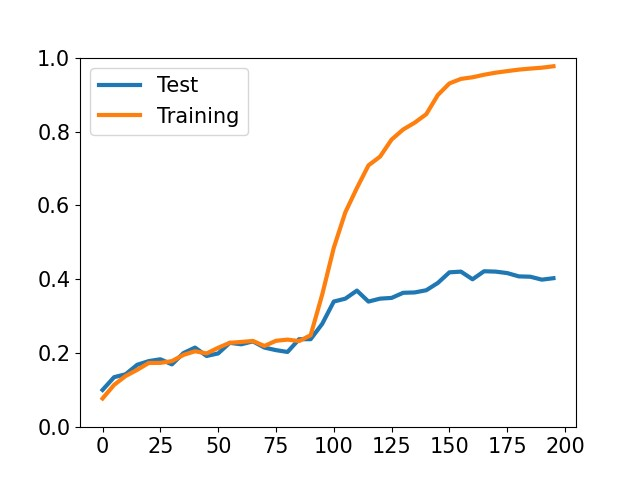
\includegraphics[width = 0.5\textwidth]{figures/clean_rare_cifar.jpg}%
\hfill
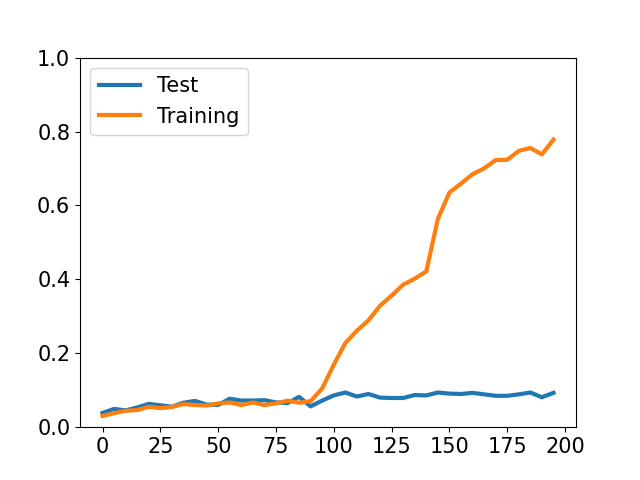
\includegraphics[width = 0.5\textwidth]{figures/adv_rare_cifar100.png}
\end{minipage}
}
\hspace*{-0.4cm}
\subfloat[Clean (left) \& Adv Acc. (right) under WRN28.]{
\label{fig:harder3}
\begin{minipage}[c]{0.55\textwidth}
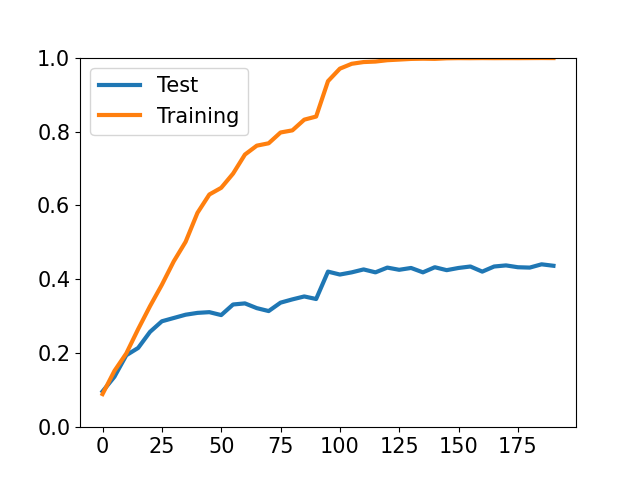
\includegraphics[width = 0.5\textwidth]{figures/wrn_clean_rare_cifar100.png}%
\hfill
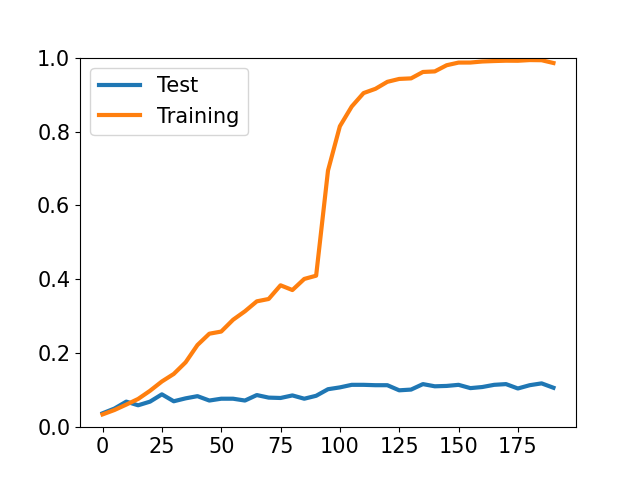
\includegraphics[width = 0.5\textwidth]{figures/wrn_adv_rare_cifar100.png}
\end{minipage}
}
\caption{Clean Accuracy and Adversarial Accuracy on \textbf{Atypical} Set of CIFAR100}
\vspace{-0.5cm}
\label{fig:rare_benefit}
\end{figure}
In this subsection, we first check whether fitting atypical samples in adversarial training can effectively help the model correctly and robustly predict the atypical samples in the test set. We apply PGD adversarial training~\cite{madry2017towards} on original CIFAR~100 dataset for 200 epochs and evaluate the model's clean accuracy and adversarial accuracy on training atypical set $\mathcal{D}_\text{atyp}=\{x_i \in \mathcal{D}: \text{mem}(x_i)> 0.15\}$ and its corresponding test atypical set $\mathcal{D}_\text{atyp}' = \{x'_j \in \mathcal{D}': \text{infl}(x_i,x'_j)> 0.15, \text{for } \forall x_i\in \mathcal{D}_\text{atyp}\}$. In Fig.~\ref{fig:rare_benefit}, we report the algorithm's performance (clean \& adv. acc.) on these atypical sets along with the training process. From the results, we observe that both ResNet18 and WRN28 are capable to memorize all clean atypical samples and most adversarial atypical samples, since they both achieve $\approx100\%$ clean accuracy and high adversarial accuracy ($\approx80\%$ and $100\%$, respectively) on the training atypical set. 
As the training goes, the models' clean accuracy on the test atypical set gradually improves and finally approaches 40\%. 
However, their adversarial robustness keep constant around 10\% from the beginning epochs to the last ones, no matter how high the training performance is. 
These results suggest that the memorizing atypical samples in adversarial training may only improve their test clean accuracy, but hardly help their adversarial robustness. Recall that in CIFAR100, atypical set $\mathcal{D}_\text{atyp}$ (with memorization value > 0.15) covers 40\% samples of the whole dataset. Completely failing on the adversarial robustness of atypical samples could be one important reason that contributes to the poor robustness generalization of DNNs~\cite{rice2020overfitting}.

As the previous theoretical study~\cite{schmidt2018adversarially} states, for a model to have good robustness generalization performance, it always demands a training set with much larger amount of samples, than a model to have good clean accuracy generalization. In our case, the sub-population of each particular atypical sample has very low frequency to appear in the training set, and it is always deviated from the main sub-population. Thus, in the sub-population of this atypical sample, it is equivalent to a classification task based on an extremely small dataset, with one or a few training samples given. Therefore, the adversarial robustness of atypical samples can be extremely hard to generalize. 
%\han{Note that the sub-population of each particular atypical sample has very low frequency to appear in the training set and it is always deviated from the main sub-population. Thus, for DNNs to classify the samples in the sub-population of this atypical sample, it is equivalent to a claication }



\vspace{-0.2cm}
\subsection{Memorizing Atypical Samples Hurts Typical Samples' Performance}\label{sec:pre2}
\vspace{-0.2cm}

%\jt{for Figure 2, Because of the high performance of clean performance, currently the difference of adversarial performance with different portions of atypical examples is not such obvious. can we put all adversarial performance in one figure and the clean performance in the other? In this way, I think the difference will be much more obvious}

In this subsection, we further observe that fitting atypical samples will even bring negative effects on ``typical'' samples. Here, we define ``typical'' samples as the subset of training set $\mathcal{D}$ which have low memorization value: $\mathcal{D}_\text{typ} = \{x_i\in\mathcal{D}:\text{mem}(x_i)<0.02\}$. It means that they are not fitted by memorization and are from the main sub-population in their class. To define the test typical set $\mathcal{D}'_\text{typ}$, we exclude all test samples which have high influence values from any atypical training samples, and also exclude the samples that using ERM algorithm $\mathcal{A}$ has low success rate to predict (the samples which cannot be learned from $\mathcal{D}$): $\mathcal{D}'_\text{typ} = \mathcal{D}' - \{x'_j: \text{infl}(x_i,x'_j)> 0.02, \text{for } \forall x_i\in \mathcal{D}_\text{atyp}\} \cup \{x'_j: \text{Pr.}_{F\leftarrow\mathcal{A}(\mathcal{D})}(F(x'_j) = y_j) < 0.8\}$.

\begin{figure}[t]
\centering
\hspace*{-1cm}
\subfloat[Clean (left) \& Adv Acc. (right) under ResNet18.]{
\label{fig:hurt1}
\begin{minipage}[c]{0.55\textwidth}
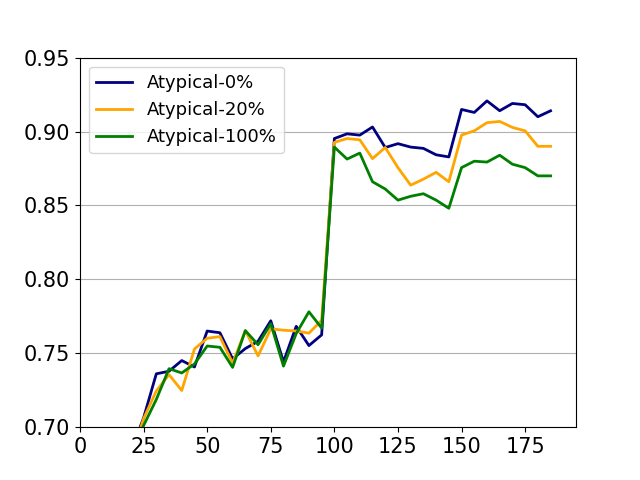
\includegraphics[width = 0.5\textwidth]{figures/poison_clean_ResNet18.png}%
\hfill
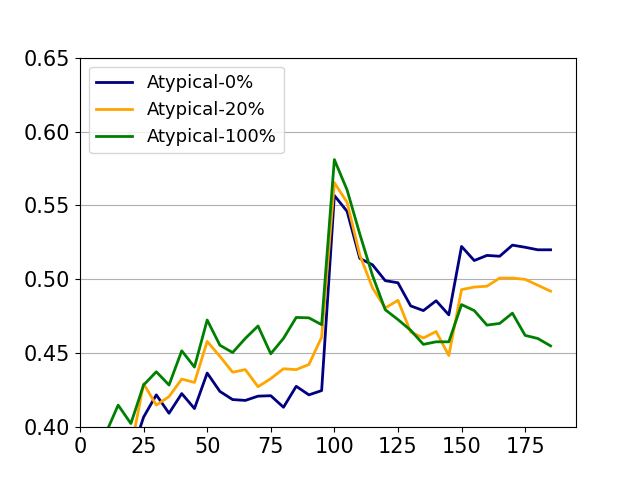
\includegraphics[width = 0.5\textwidth]{figures/poison_adv_ResNet18.png}
\end{minipage}
}
\hspace*{-0.4cm}
\subfloat[Clean (left) \& Adv Acc. (right) under WRN28.]{
\label{fig:hurt2}
\begin{minipage}[c]{0.55\textwidth}
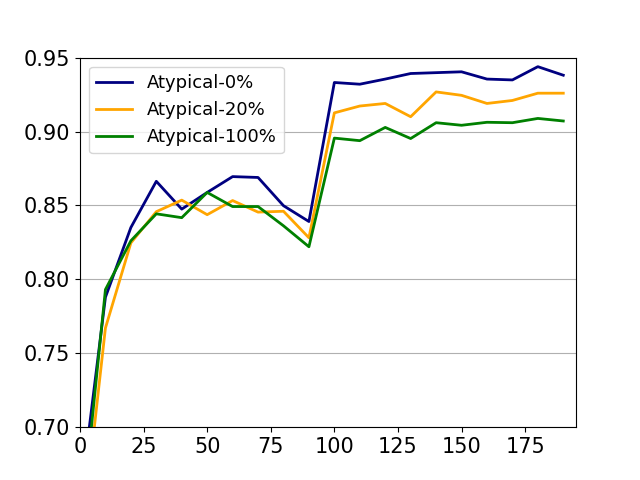
\includegraphics[width = 0.5\textwidth]{figures/poison_clean_WRN.png}%
\hfill
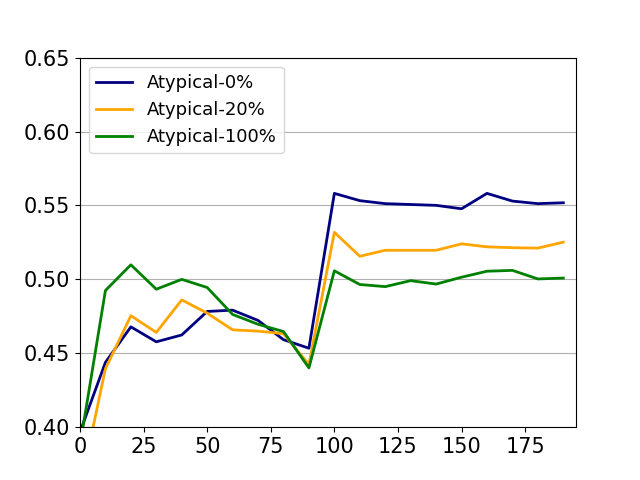
\includegraphics[width = 0.5\textwidth]{figures/poison_adv_WRN.png}
\end{minipage}
}
\caption{Clean Accuracy and Adversarial Accuracy on \textbf{Typical} Set of CIFAR100}
\vspace{-0.5cm}
\label{fig:hurt}
\end{figure}
To demonstrate the negative effect from fitting atypical samples, we conduct PGD adversarial training~\cite{madry2017towards} for several trails on resampled CIFAR100 datasets: each dataset is constructed with the whole training typical set $\mathcal{D}_\text{typ}$, and a part of the training atypical set $\mathcal{D}_\text{atyp}$ (randomly sample 0\%, 20\% and 100\% in $\mathcal{D}_\text{atyp}$). In Fig.~\ref{fig:hurt}, we report the adversarially trained model's clean and adversarial accuracy on the test typical set $\mathcal{D}_\text{typ}'$ and check the impact of atypical samples on the typical samples. From the results, we find that the amount of atypical samples makes a significant influence on the typical samples. For example, under ResNet18, an adversarially trained model without atypical samples has 92\% clean accuracy and 52\% adversarial accuracy on the test typical samples (on the last epochs). While, the model trained with all atypical samples included only has 85\% and 44\% clean \& adv. accuracy, respectively. 
These results suggest: the more atypical samples exist in training set, the poorer performance the model will have on $\mathcal{D}'_\text{typ}$. In other words, these atypical samples act more like ``poisoning'' samples~\cite{biggio2012poisoning, xu2019adversarial} which can deteriorate the model's performance on typical samples and consequently hurt the overall performance. 


\noindent\textbf{Poisoning Atypical Samples} A natural question is what kind of atypical samples are likely to ``poison'' model robustness and why? Different from previous literature about poisoning samples in traditional ERM, which assume that poisoning samples are most mis-labeled samples~\cite{li2020gradient}, CIFAR100 is a clean dataset with no or very few wrong labels. However, we hypothesize that the atypical samples which poison the model performance might pertain some features of a ``wrong'' class. Recall that atypical samples are always distinct from the main data distribution in their labeled class, it is likely that they are closer to the distribution of a ``wrong'' class. As shown in  Fig.~\ref{fig:atypical_samples}, an atypical ``plate'' is visually very similar to images in ``apple''. If the model memorizes this atypical ``plate'' and predicts any samples with similar features to be ``plate'', the model cannot distinguish between ``apple'' and ``plate''. As a simple verification to this hypothesis, in Table~\ref{Tab:dist}, we empirically show that atypical samples can cause adversarial training to produce ``less-discriminative'' representations among different classes. Under the same experimental setting and the models above, we measure the average \textit{Cosine Distance (CD)~\footnotemark} of the models' pen-ultimate layer representation output, for each pair of samples (in the training typical set $\mathcal{D}_\text{typ}$) from different classes. Table~\ref{Tab:dist} shows that in adversarial training, fitting more atypical samples will result in a smaller distance for the representations of samples in different classes. It suggests that with atypical samples, DNNs learn more similar and mixed representations for different classes, which can degrade the typical samples' test performance.
\begin{table}[h]
\vspace{-0.5cm}
\small
\centering
\setlength{\tabcolsep}{12pt}
\caption{Class-wise Cosine Distance of Representations of Typical Samples}
\begin{tabular}{c|ccc}
\hline
\# of Atypical Samples & 0\% &20\% &100\%\\
\hline
ResNet18 & 0.66 & 0.62  & 0.59\\
\hline
WRN28 &0.64 & 0.61 & 0.57\\
\hline
\end{tabular}
\vspace{-0.4cm}
\label{Tab:dist}
\end{table}

\footnotetext{Cosine Distance: $\E_{x_1,x_2} [\frac{h(x_1)\cdot h(x_2)}{||h(x_1)||_2\cdot||h(x_2)||_2}]$, where $h(\cdot)$ is the pen-ultimate layer output of DNN model $F(\cdot)$, and $x_1,  x_2\in \mathcal{D}_\text{typ}$ and from different classes.}


It is also worth to mention that this poisoning phenomenon does not appear in the traditional ERM algorithm (results in Appendix~\ref{app:pre}). In ERM, memorizing atypical samples will neither hurt typical sample's performance or degrade the feature space discrimination. A possible explanation is that adversarially trained models use more ``semantically meaningful'' features for prediction~\cite{tsipras2018robustness, ilyas2019adversarial}. During adversarial training, the models will not only memorize the labels of atypical samples, but also their semantic features. As a result, the adversarial trained DNNs will construct more mixed concepts of features, if the ``poisoning'' atypical samples exist.


\begin{figure}[t]
\subfloat{
\label{fig:poison_pair1}
\begin{minipage}[c]{0.5\textwidth}
\centering
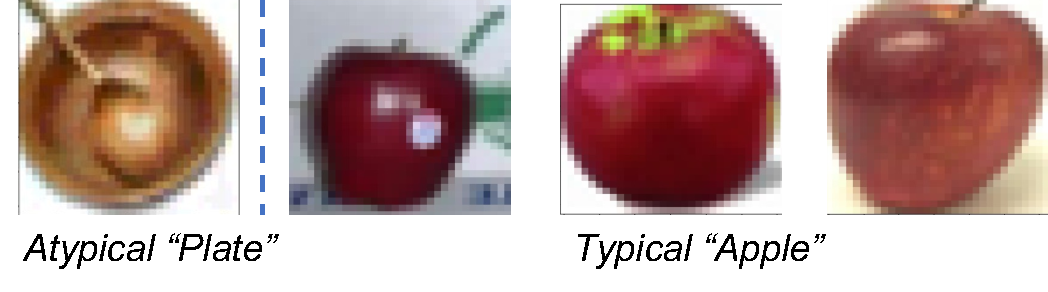
\includegraphics[width = 0.8\textwidth]{figures/poison_pair1.pdf}
\end{minipage}
}
\subfloat{\label{fig:poison_pair2}
\begin{minipage}[c]{0.5\textwidth}
\centering
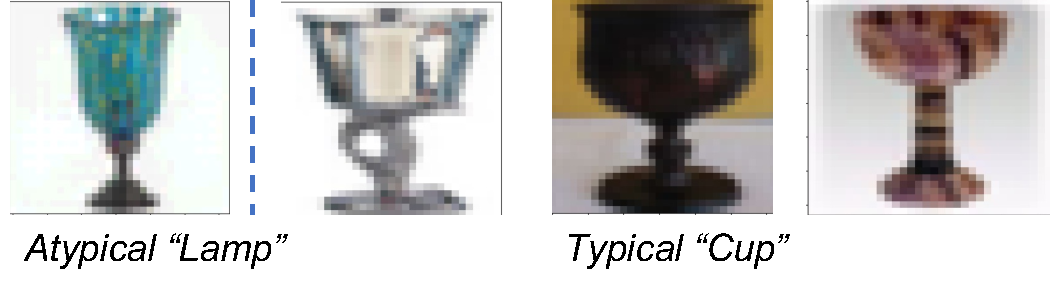
\includegraphics[width = 0.8\textwidth]{figures/poison_pair2.pdf}
\end{minipage}
}
\caption{Examples of Poisoning Atypical Samples}
\vspace{-0.4cm}
\label{fig:atypical_samples}
\end{figure}

% \begin{figure*}[t]
%   \centering
%   \includegraphics[width=\textwidth]{cvpr_2022/framework_4.pdf}
%   \vspace{-5mm}
%   \caption{Illustration of our framework. (a) \textbf{Target-aware Transformer}. Conditioned on the teacher feature and the student feature, the transformation map Corre. is computed and then applied on the student feature to reconfigure itself, which is then asked to minimize the L$_2$ loss with the corresponding teacher feature. (b) \textbf{Patch-group Distillation}. Both teacher and student features are to be sliced and rearranged as groups for distillation. By concatenating the patches within a group, we explicitly introduce the spatial correlation among the patches beyond the patches themselves. (c) \textbf{Anchor-point Distillation}. Each color indicates a region. We use average pooling to extract the \textit{anchor} within a local area of the given feature map, forming the new feature map of a smaller size. The generated anchor-point features will participate in the distillation.}
%   \label{fig:framework}
%   \vspace{-5mm}
% \end{figure*}

%-------------------------------------------------------------------------
%\usepackage{amsmath}
%\usepackage{autobreak}
\section{Method}
\label{sec:method}
% There is a temptation, though, to let the student perfectly mimic the teacher, which does not appear to be viable in reality because student is inferior to teacher in learning capacities. Rather, we introduce the cross-attention to assist the feature matching between student and teacher. The cross-attention is conditioned by a pair of teacher feature and student feature that reflects the context of two given features. In practice \cite{Cho2019OnTE,Ji2021ShowAA,Chen2020CrossLayerDW}, it's hard for the student to directly match (\ie reconstruct) a teacher layer. Prior methods used an attention \textit{weight} to regulate the loss function or decide the allocation of the teacher layers to student, which is a global manner. In contrast, our method allows the student to perform self-assessment through the cross-attention and be aware of the difference and similarity compared to teacher feature, which can facilitate the knowledge transfer. (See Figure~\ref{fig:framework} (a)).


% In this section, we will provide a detailed description of the proposed cross-modality distillation method. The overall architecture is illustrated by Fig. 1. Our architecture consists of three branch: Lidar-based detector branch, Multi-view based detector branch and the cross-modal supervision. We will introduce cross-modal supervision components in detail in the following sections. 

\begin{figure*}[t!]
  \centering
  % \vspace{0.2cm}
  \includegraphics[width=\textwidth]{cvpr_2022/iccv_fig4.drawio.png}
  % \vspace{-5mm}
  \caption{\textbf{Overall Framework of TiG-BEV,} which contains a pre-trained LiDAR-based detector as teacher, a camera-based detector as student, and a target inner-geometry scheme for cross-model learning. Our proposed learning paradigm effectively transfers the inner-geometry semantics of the LiDAR modality via two components, an inner-depth supervision (Section~\ref{sec:Inner-depth Supervision}) for foreground relative depth, and an inner-feature BEV distillation (Section~\ref{sec:Inner-feature BEV Distillation}) from both channel-wise and keypoint-wise.}
  \label{fig:framework}
  % \vspace{0.3cm}
  % \vspace{-5mm}
\end{figure*}

The overall architecture of TiG-BEV is shown in Figure~\ref{fig:framework}, which consists of three components: the student camera-based detector, the teacher LiDAR-based detector, and our proposed target inner-geometry learning scheme. In Section~\ref{sec:Baseline Models}, we first introduce the adopted baseline models. Then, we specifically illustrate the designs of TiG-BEV for inner-depth supervision in Section~\ref{sec:Inner-depth Supervision} and inner-BEV feature distillation in Section~\ref{sec:Inner-feature BEV Distillation}. Finally in Section~\ref{sec:overall_loss}, we present the overall loss of our TiG-BEV for LiDAR-to-camera learning.

\subsection{Baseline Models}
\label{sec:Baseline Models}
\paragraph{Student Camera-based Detector.}
By default, we adopt BEVDepth~\cite{b7} as our student camera-based detector for multi-view 3D object detection. 
Given the input multi-view images (normally 6 views for a scene), the student model first utilizes a shared 2D backbone and FPN module~\cite{b54} to extract the $C$-channel visual features $\{F_i\}_{i=1}^6$, where $F_i \in {\mathbb{R}^{C\times H_v\times W_v}}$, and $H_v, W_v$ denote the size of feature maps. These features are fed into a shared depth network to generate the categorical depth map~\cite{b51}, $\{D_i\}_{i=1}^6$, where ${D_i}\in {\mathbb{R}^{D\times H_v\times W_v}}$, where D denotes the pre-defined number of depth bins. During training, BEVDepth adopts dense depth supervision for the predicted depth maps, which projects the paired LiDAR input onto multi-view image planes to construct pixel-by-pixel absolute depth ground truth, $\{D_i^{gt}\}_{i=1}^6$, where ${D_i^{gt}}\in {\mathbb{R}^{1\times H_v\times W_v}}$. 
Then, following~\cite{b20}, the multi-view visual features are projected into a unified BEV representation via the predicted depth maps, which is further encoded by a BEV encoder, denoted as $F^{2d}_{\rm bev}\in {\mathbb{R}^{C\times H_{\rm bev}\times W_{\rm bev}}}$. Finally, the detection heads are applied on top to predict objects in 3D space. We represent the two basic losses of the student model as $\mathcal{L}_{\rm{depth}}^{A}$ and $\mathcal{L}_{\rm{det}}$, respectively denoting the Binary Cross Entropy loss for dense absolute depth values and the 3D detection loss.

\paragraph{Teacher LiDAR-based Detector.}
We select the popular LiDAR detector CenterPoint~\cite{b53} as the teacher for target inner-geometry learning. Given the input point cloud data, CenterPoint voxelizes into grid-based data and utilizes a 3D backbone to obtain the $C$-channel LiDAR BEV feature $F^{3d}_{\rm bev}\in {\mathbb{R}^{C\times H_{\rm bev}\times W_{\rm bev}}}$, which has the same feature size as $F^{2d}_{\rm bev}$ from the student detector. As the CenterPoint has been well pre-trained, $F^{3d}_{bev}$ can provide the student BEV feature with sufficient geometric and semantic knowledge, espeically in the target foreground areas. Note that the LiDAR-based teacher is merely required during training for cross-modal learning, and for inference, only multi-view images are token as input for the camera-based detector.


% To adapt the method to semantic segmentation, we introduce the hierarchical distillation, which is more computationally practical, to transfer the feature and long-range dependency, respectively. 

%This section first presents the general formulation of the proposed method in the scope of image classification. 
% We then explain the insights of the model. 
%In order to adapt to semantic segmentation, we introduce the hierarchical distillation consisting of patch-group and anchor-point distillation to transfer the  feature and global dependency respectively.

% \subsection{Absolute Depth Supervision}
% \label{sec:formulation}
% % Suppose that teacher and student are two \ky{differentiable} functions, which are parameterized by CNNs in this work and denoted by $T$ and $S$. 
% % Suppose the teacher and the student are two convolutional neural networks, denoted by $T$ and $S$.
% % $F^T\in {\mathbb{R}^{H\times W\times C}}$ and ${F^S}\in \mathbb{R}^{H\times W\times C^{'}}$ denote the teacher feature and student feature respectively, where $H$ and $W$ are the height and width of the feature map, and $C$ represents the channel numbers. In the pioneer work~\cite{Hinton2015DistillingTK}, the distillation loss is formulated by a distance of features that come from the last layer of the networks. For example, in the image classification domain, it refers to the  ``logits'' before going in the softmax layer and cross-entropy loss. 
% Following early work BEVDepth, we propose to supervise the intermediate depth prediction ${D_i}^{pred}$ using ground-truth ${D_i}^{gt}$ generated from point clouds data $P$. Specifically, we create the depth maps by the Depth Generator and detail the depth generation process below.

% Donated $R_i\in{\mathbb{R}^{3\times 3}}$ and $t_i\in{\mathbb{R}^{3}}$ as the rotation and translation matrix from the ego coordinate to the camera coordinate of the $i^{th}$ view, and donated $K_i\in{\mathbb{R}^{3\times 3}}$ as the intrinsic parameter of the $i^{th}$ camera. Then we can obtain ${D_i}^{gt}$ by:
% \begin{equation}
%     \hat{P_i^{img}}(u{D_i}^{gt}, v{D_i}^{gt}, {D_i}^{gt}) = K_{i}(R_i P + t_i),
% \end{equation}
% where $u$ and $v$ denote coordinates in pixel coordinate. 

% Then we apply one hot encoding to ${D_i}^{gt}$ considering the depth estimation as a classification problem of the depth distribution. For the defined depth bins $b_i$, we interpret the $D$ Softmax scores, $p^{k}_i$, $k=1,..,D$, and choose the final prediction depth $b^{k}_i$ at highest prediction confidence bin. Finally we adopt Binary Cross Entropy as absolute depth supervision loss to optimize our predicted depth distribution ${D_i}^{pred}$ as shown in Eq.~\ref{eq:BCE},
% \begin{equation}
%     \mathcal{L}_{\rm{Adepth}} = -\sum_{k=1}^D{(y^k\log(p^k) + (1 - y^k)\log(1 - p^k))}
%     \label{eq:BCE}
% \end{equation}
% where $y^k$ is either zero or one indicating whether $k$ is the discrete ground truth depth.

% With the help of absolute depth supervision, camera branch will be able to produce reliable ${D_i}^{pred}$. 
 %\noindent we finally can get GT depth map in image coordinates $P_i^{img}(u, v,  d)$, where $u$ and $v$ denote coordinates in pixel coordinate. If the 2.5D projection of a certain point cloud does not fall into the $i^{th}$ view, we simply discard it. See Fig.~\ref{fig:bevdepth} for an example of the projection result. Then, to align the shape between the projected point clouds and the predicted depth, a \textit{min pooling} and a \textit{one hot} are adopted on $P_i^{img}$. We jointly define these two operations as $\phi$, the resulting $D^{gt}$ can thus be written in Eq.~\ref{dgt}. As for the depth loss $L_{depth}$, we simply adopt Binary Cross Entropy. 


\vspace{0.1cm}
\subsection{Inner-depth Supervision}
\label{sec:Inner-depth Supervision}

In addition to the dense absolute depth supervision, we propose to guide the student model to learn the inner-depth geometries in different target foreground areas. As shown in Figure~\ref{fig:relative_depth} (a), for the instance level, the existing absolute depth supervision with categorical representation ignores the relative structural information inside each object and provide no explicit fine-grained depth signals. Therefore, we propose to additionally conduct inner-depth supervision with continuous values from the LiDAR projected depth maps shown in Figure~\ref{fig:relative_depth} (b), which effectively boosts the network to capture the inner-geometry of object targets.

\paragraph{Foreground Target Localization.}
To accurately obtain the inner-depth values, we first localize the foreground pixels for each object targets in the depth maps. Given the ground-truth 3D bounding boxes, we extract the corresponding 3D LiDAR points inside the box for each object target, and project them onto different image planes. In this way, we can attain the pixels within foreground object areas on both the predicted and ground-truth depth maps, $\{D_i, D_i^{gt}\}_{i=1}^6$. The foreground pixels can roughly depict the geometric contour of different target objects and well improve the subsequent inner-depth learning. We taking the $i$-th view as an example and omit the index $i$ in the following texts for simplicity. Suppose there exist $M$ target objects on the image, we denote the foreground depth-value set for the $M$ objects as $\{S_j, S_j^{gt}\}_{j=1}^M$, where each $\{S_j, S_j^{gt}\}$ includes the foreground categorical depth prediction and ground-truth depth values for the $j$-th target.

\paragraph{Continuous Depth Representation.}
Different from the categorical representation of absolute depth values, we represent the predicted inner depth of foreground targets by continuous values, which reflects more fine-grained geometric variations. For pixel $(x, y)$ of the $j$-th target object $S_j$, the predicted possibility of $k$-th depth bin is denoted as $S_j(x, y)[k]$, where $1\le k\le D$. Referring to MonoDETR~\cite{b47,b48}, we calculate the continuous depth value $d_j(x, y)$ for the pixel $(x, y)$ as
 \begin{equation}
 \label{eq:FM}
 \begin{aligned}
    d_j(x, y) = {\sum_{k=1}^D({d[k]\cdot S_j(x, y)[k]})},
 \end{aligned}
 \end{equation}
where $d[k]$ denotes the depth value of the $k$-th bin center. By this, we convert the categorical depth prediction of different target objects, $\{S_j\}_{j=1}^M$, into continuous representations, denoted as $\{\hat{S_j}\}_{j=1}^M$.

\begin{figure}[!t]
% \vspace{-0.5cm}
    \centering
    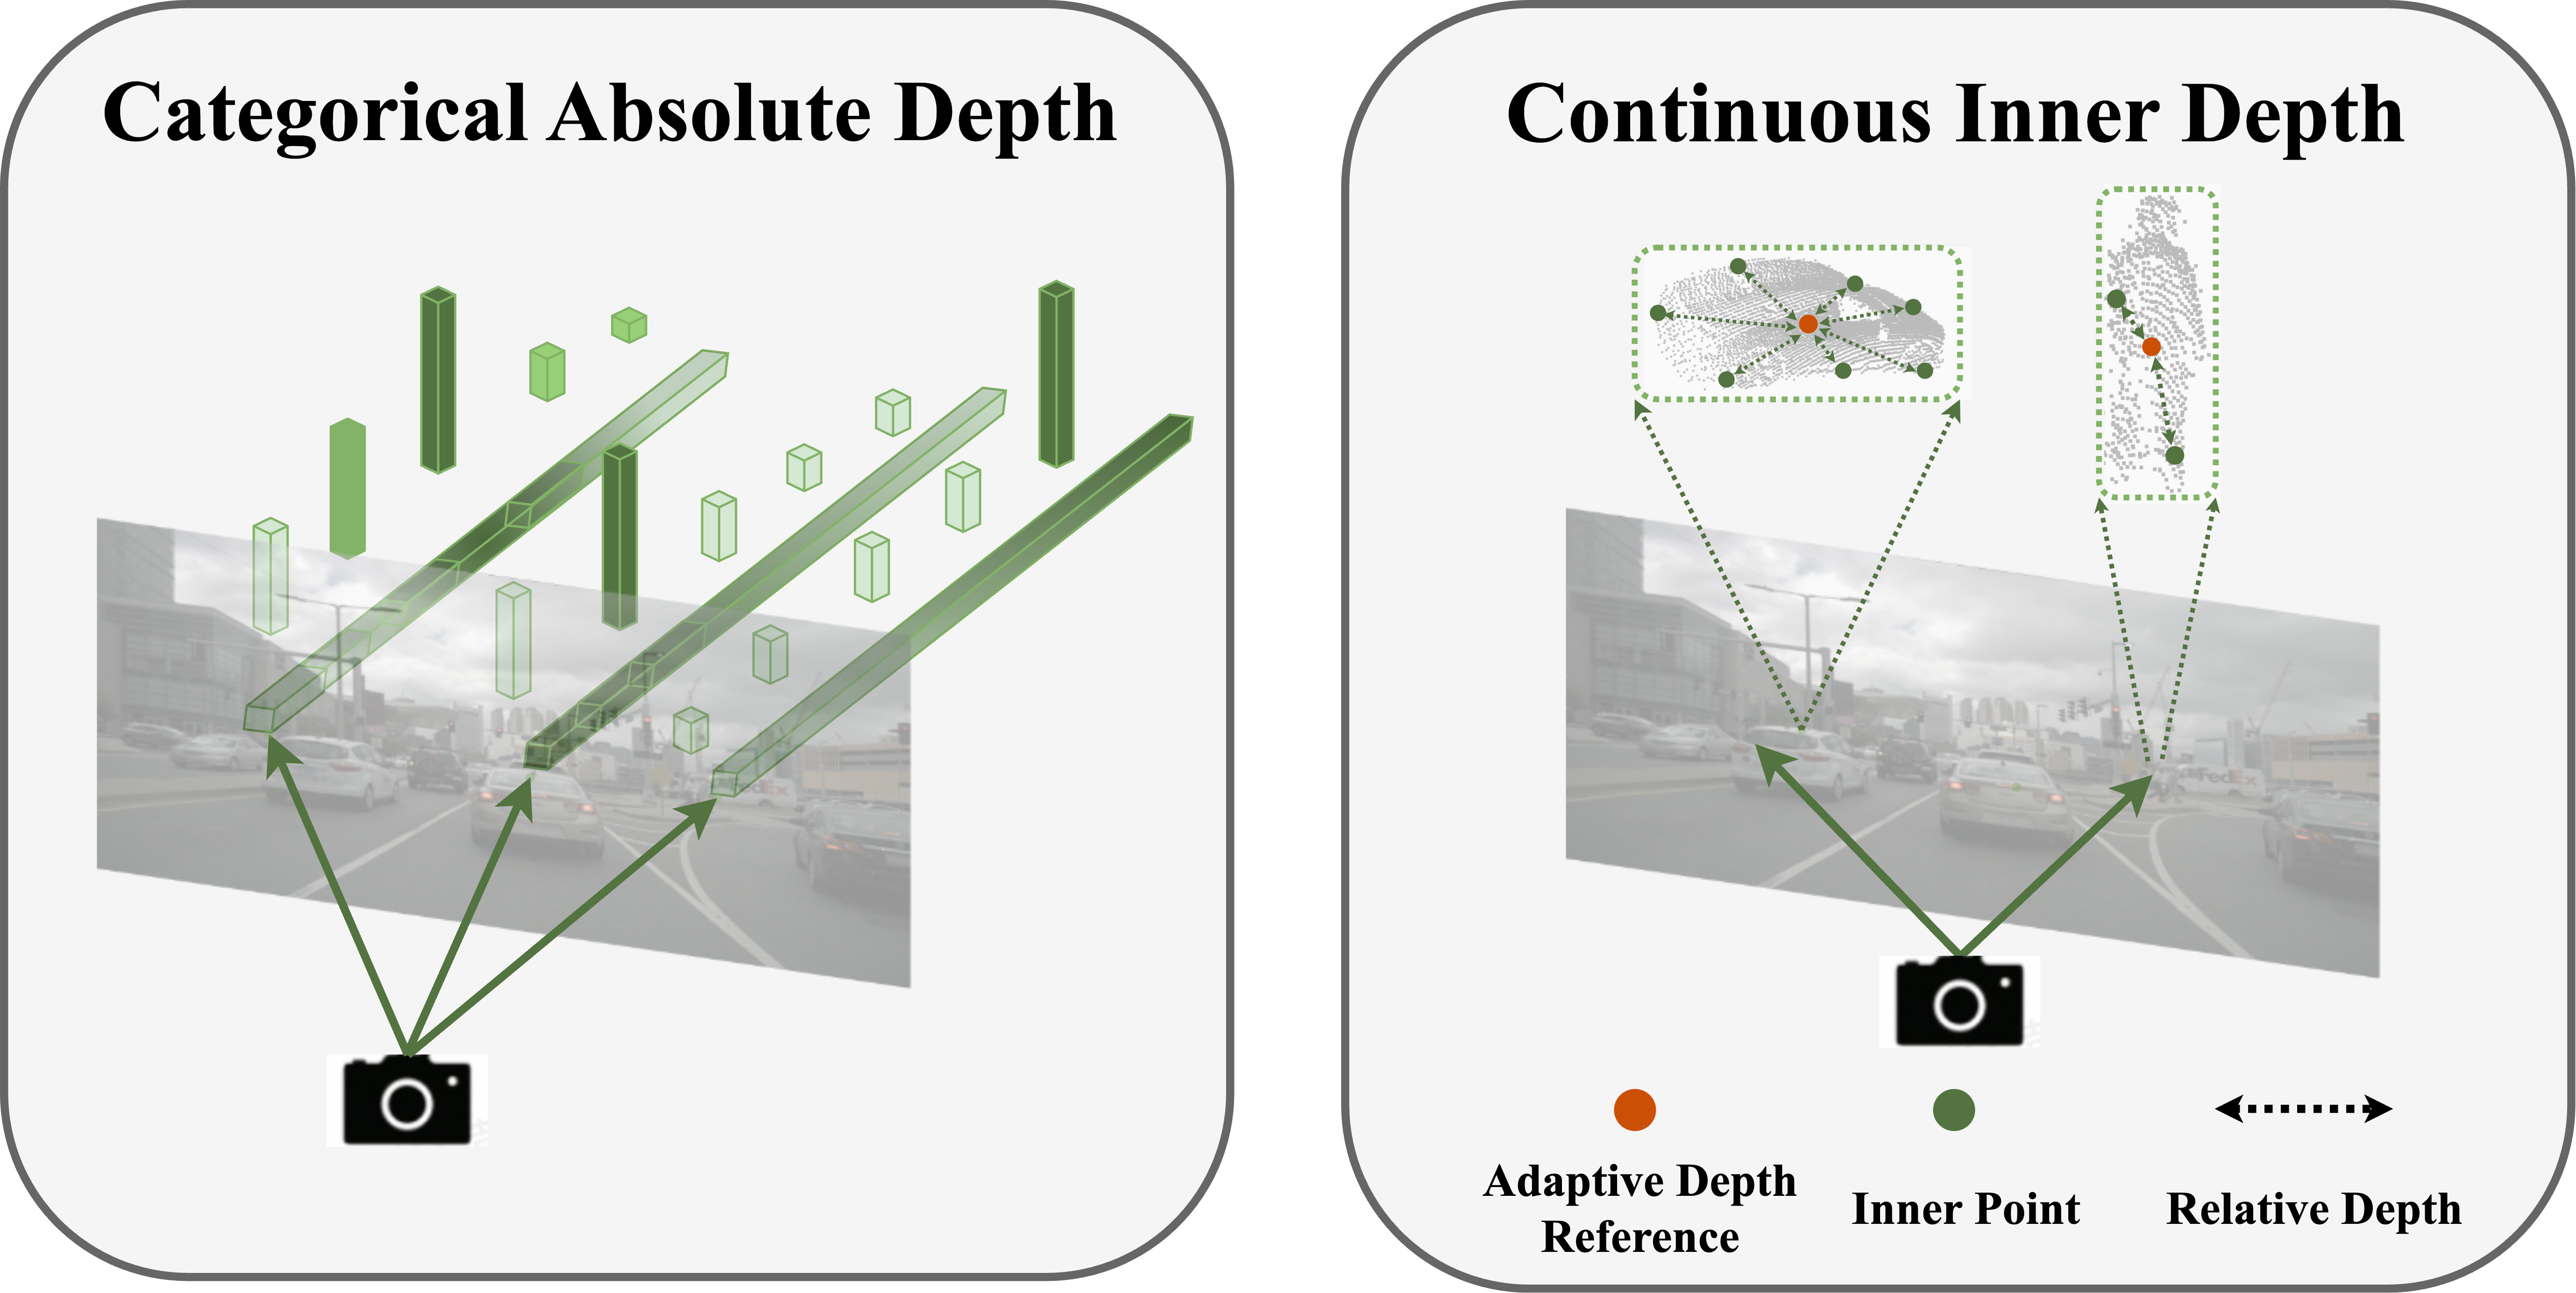
\includegraphics[scale=0.042]{cvpr_2022/iccv_fig5.drawio.png}
    \caption{\textbf{Comparison of Categorical Absolute Depth and Continuous Inner Depth.} We adopt the inner-depth supervision with continuous depth values to guide the camera-based student to learn local spatial structures of foreground object targets.
    }
    \label{fig:relative_depth}
    % \vspace{-0.8cm}
\end{figure}

%Start with $N$ ground truth 3D bounding boxes $\bm{B_{gt}}= \{\bm{b}_{i}\}_{i=1}^{N}$, which contains box center position, size and heading angle. We then obtain points in each 3D bounding boxes $\bm{P_{gt}}= \{\bm{P}^{pc}_i\}_{i=1}^{N}$, ${P}^{pc}_i$ means point clouds $P$ within 3d bounding box ${b}_{i}$. Take an object instance as example, we project ${P}^{pc}_i$ on image coordinate. 

%\begin{equation}
%    \hat{P_i^{}}(ud, vd, d) = K_{i}(R_i P_{i} + t_i),
%\end{equation}
 %In the section 3.1, we consider the depth estimation as a classification problem of the depth distribution. For the defined depth bins $b_i$, we interpret the $D$ Softmax scores, $p_k$, $k=1,..,D$, and choose the final prediction depth $b^{k}_i$ at highest prediction confidence bin. 

% In the absolute depth supervision, we apply one hot encoding to ${D_i}^{gt}$ considering the depth estimation as a classification problem of the depth distribution, first adopted in BEVDepth \cite{b7}. We divided the depth distance into D depth bins, the depth-bin-centers set denoted as ${\mathbf{B_i}=\{b^1_i, b^2_i,..., b^k_i,... b^D_i\}}$ , and we interpret the $D$ Softmax scores, $p^{k}_i$, $k=1,..,D$ at each pixel as probabilities over the ${\mathbf{B_i}}$ vector, and choose the final prediction depth $b^{k}_i$ at highest prediction confidence bin. 
%  \begin{equation}
%  \label{eq:FM}
%  \begin{aligned}
%     D_i = b^{k}_i {\max_{k=1}^D {{p^{k}_i}}}.
%  \end{aligned}
%  \end{equation}
% Here, we want to calculate the exact relative depth for different pixels within the target, the discrete depth prediction like above is not enough to express the tiny depth difference. Thus, for the further accurate prediction depth and can be used for the relative depth relation among different pixels within the certain ROI, we calculate the final depth value $\hat{D_i}$ by the hybrid mean regression as follow:
%  \begin{equation}
%  \label{eq:FM}
%  \begin{aligned}
%     {\hat{D_i}} = {\sum_{k=1}^D {{b^{k}_i}{p^{k}_i}}}.
%  \end{aligned}
%  \end{equation}
 % Compared the discrete depth prediction, we do not predict the depth as the chosen likely bin. This enables us to predict smooth depth without the discriminative artifacts, which helps to obtain the complete representation of the geometry depth.  
 
 \paragraph{Adaptive Depth Reference.}
 To calculate the relative depth values, we propose to utilize an adaptive depth reference for different foreground targets.
 Specifically, according to the predicted continuous depth values in $\{\hat{S_j}\}_{j=1}^M$, we select the pixel with the smallest depth prediction error as the reference point for each target, and correspondingly set its depth value as the depth reference, as shown in Figure~\ref{fig:relative_depth}. For the $j$-th target with the ground-truth inner-depth $\{\hat{S_j}, \hat{S^{gt}_j}\}_{j=1}^M$, we calculate the depth reference point $(x_r, y_r)$ by
  \begin{equation}
 \label{eq:FM}
 \begin{aligned}
    (x_r, y_r) = \mathop{\text{Argmin}}_{(x, y)\in \hat{S_j}} \left ({S^{gt}_j}(x, y) - {\hat{S_j}}(x, y)\right ).
 \end{aligned}
 \end{equation}
 Then, the predicted and ground-truth reference depth values are denoted as $d_j(x_r, y_r)$ and $d^{gt}_j(x_r, y_r)$, respectively. By adaptively selecting the reference point with the smallest error, the inner-depth distribution can dynamically adapt to objects with different shapes and appearances, which stabilizes the network learning for some truncated and occluded objects.

\paragraph{Inner-depth Calculation.}
On top of the reference depth value, we calculate the relative depth values within the foreground area of each target object. For pixel $(x, y)$ of the $j$-th target $\{\hat{S_j}, S_j^{gt}\}$, the predicted and ground-truth inner-depth values are formulated as
\begin{equation}
 \label{eq:FM}
 \begin{aligned}
    rd_j(x, y) &= d_j(x, y) - d_j(x_r, y_r),\\
    rd^{gt}_j(x, y) &= d^{gt}_j(x, y) - d^{gt}_j(x_r, y_r).
 \end{aligned}
 \end{equation}
 We denote the obtained relative depth-value sets for $M$ target objects as $\{\hat{R_j}, R_j^{gt}\}_{j=1}^M$. Finally, we supervise the inner-depth prediction of the student detector by an L2 loss, formulated as
 \begin{equation}
\label{eq:FM}
    \mathcal{L}_{\rm{depth}}^{R} = \sum_{j=1}^M ||\hat{R}_{j}-R^{gt}_{j}||_2.
\end{equation}
 
%  When we set the inner point and the reference point within the ROI, we can define the two relative depth sets ${\mathbf{\hat{D}}^{gt}}$ ${\mathbf{\hat{D}}^{pred}}$ of the pixels with cardinality ${M}$. 
% \begin{equation}
%     {\mathbf{\hat{D}}^{gt}} = 
% \left[{\hat{D}^{gt}_{1r},\hat{D}^{gt}_{2r},\cdots,\hat{D}^{gt}_{ir},\hat{D}^{gt}_{Mr}}\right].
% \end{equation}
% \begin{equation}
%     {\mathbf{\hat{D}}^{pred}} = 
% \left[{\hat{D}^{pred}_{1r},\hat{D}^{pred}_{2r},\cdots,\hat{D}^{pred}_{ir},\hat{D}^{pred}_{Mr}}\right].
% \end{equation}
%  where the ${\hat{D}_{ir}^{gt}}=\hat{D}_i^{gt}-\hat{D}_r^{gt}$ and ${\hat{D}_{ir}^{pred}=\hat{D}_i^{pred}-\hat{D}_r^{pred}}$ denotes the relative depth distance of the lidar pixels and cam pixels. 
 
%  To obtain the inner-geomtry depth relation from the lidar points, we minimize the discrepancy between the above sets in a one-to-one relative spatial matching manner. 
% \begin{equation}
% \label{eq:FM}
%     \mathcal{L}_{\rm{Rdepth}} = ||{\mathbf{\hat{D}}^{gt}}-{\mathbf{\hat{D}}^{pred}}||_2 = \sum_{i=1}^M ||\hat{D}^{gt}_{ir}-\hat{D}^{pred}_{ir}||_2.
% \end{equation}
%% \KY{focus on semantic mismatch}
%\noindent This formulation assumes that the semantic distributions of the teacher and the student match exactly. 
% However, a recent study~\cite{Cho2019OnTE} observes that small students are inefficient to mimic large teachers. 
%However, as mentioned earlier, for the feature maps of the teacher network, which usually encompasses more layers and larger feature channels, the spatial information of the same pixel location contains a richer semantic information compare to the student network. Directly regressing the features in a pixel-wise manner may lead to suboptimal distillation results. 
% has a stronger learning capability (\eg larger receptive field) and richer representation. That means the semantic of spatial components of teacher and student usually varies. Directly linking the teacher and student by spatial order may trigger the issues of semantic mismatch and lead to sub-optimal results.
% \KY{this is not helping the story, size difference is one reason that KD is hard. but our approach does not help in this way} 
% As the teacher grows in capacity and accuracy, the student often finds it difficult to emulate the teacher. 
% To this end, we propose to guide the whole student to mimic each spatial component of the teacher respectively. In this way, we can increase the matching capability and subsequently improve the knowledge distillation performance.

%This formulation does not consider the gap of expressivity and the exact semantic distance between $f^s_i$ and $f^t_i$, which may introduce bias. To address the limitation of Eq. \ref{eq:FM}, we reconfigure each elements in set $f^s$ by a target-aware transformer. 
%A straightforward solution is to measure the semantic distance between the elements of two sets and then assign the $f^t_i$ with the most semantic-related one from $f^s$. As we will demonstrate, this is the special case of our proposed method.
%To this end, we propose a one-to-all spatial matching knowledge distillation pipeline that allows the each feature location of the teacher to teach the entire student features in a dynamic manner.
%To make the whole student mimic a spatial component of the teacher, we propose the \textbf{T}arget-\textbf{a}ware \textbf{T}ransformer (\textbf{TaT}) to pixel-wisely reconfigure the semantic of student feature in the certain position.
%We propose the Target-aware Transformer (\textbf{TaT}) to pixel-wisely reconfigure the semantic of student feature in the certain position. 
%Given a spatial component (alignment target) of the teacher, we use \textbf{TaT} to guide the whole student to reconstruct the feature in its corresponding location. Conditioned on the alignment target,  \textbf{TaT} should reflect the semantic similarity with the components of the student feature. We use a linear operator to avoid changing the distribution of student semantics. The formulation of transformation operator $W^i$ can be defined as:
%Given the alignment target $f^t_i$, \textbf{TaT} is to find the weights $W^i$ that controls the flow of semantic aggregation across the student feature w.r.t the $i$-th pixel of student feature. Conditioned on the alignment target, \textbf{TaT} should reflect the semantic similarity with the components of the student feature. Also, it should be a linear operator otherwise it changes the distribution of student semantics. The formulation of $W^i$ can be defined as:
%\begin{equation}
%\label{eq:spe}
%\begin{aligned}
%   W^i&= \sigma(\langle {f^s_1},{f^t_i}\rangle,\langle {f^s_2},{f^t_i}\rangle,\dots,\langle {f^s_N},{f^t_i}\rangle)\\
%   &=[{w^i_1},{w^i_2},\dots,{w^i_N}],
%\end{aligned}
%\end{equation}
%\noindent where $f^t_i$ and $f^s_i$ denote the corresponding $i$-th components of teacher and student, $\langle \cdot,\cdot \rangle$ represents the inner-product and  $\|W^{i}\|=1$. We use inner-product to measure the semantic distance and softmax function for normalization. 
%Note that if we only reserve the entry of the maximum of $W^{'}$, it degrades to the nearest-neighbor. 
% Here $W^{i}$ is the gate that guides the semantic flow to the reconfigured point ${f^s_i}^{'}$. 



%Note this is the simple non-parametric method that only depends on the original features. To facilitate the training, we introduce the parametric method with the extra linear transformation applied on the student feature and teacher feature. We observe that parametric version performs better than non-parametric one in ablation study. Guided by the target-aware transformer, the reconfigured student feature can be formulated as: 
% \KY{why we need parameteric formulation? does non-param work? do we have the experiment? if not, consider to do this in supplementary}
% Also, the issue of semantic mismatching may occur in the channel dimension. To address this issue, we propose to partition the feature tensor along the channel dimension and performs the self-assembling in parallel:
%\begin{equation}
%\label{eq:mul-self-essem}
%    {f^s}^{'}=\sigma(\gamma(f^{s})\cdot \theta({f^t})^{\top})\cdot \phi(f^{s}),
%\end{equation}
%\noindent where $\theta(\cdot)$, $\gamma(\cdot)$ and $\phi(\cdot)$ are the linear functions consisting of $3\times 3$ conv layer plus the BN layer \cite{ioffe2015batch}. We compare the parametric \textbf{TaT} to non-parametric one to analyse the effectiveness brought by these linear functions in the Section~\ref{sec:ablation}. 
%In the case that the channel numbers of $F^S$ do not match with that of $F^T$, $\gamma(\cdot)$ can help with alignment.

% \KY{where? point the section} 
%The resulting \textbf{TaT} map ($\gamma(f^{s})\cdot \theta({f^t})^{\top}$) is of size $\mathbb{R}^{HW \times HW}$, which is acceptable considering that most classification networks have small feature map size on the top layers. On ResNet18, the spatial size of feature map in the 4-th block is, for example, $7\times7$.  \KY{discuss the complexity in the next section...}

%After reconfiguration, each component of ${f^s}^{'}$ aggregates the meaningful semantic from the original feature, which enhances the expressivity. We do not require the student to reconstruct the teacher feature in a pixel-to-pixel manner. Indeed, our model allows the student to act as a whole to mimic the teacher. The resulting ${f^s}^{'}$ is lately asked to minimize the L$_2$ loss with the teacher feature. The objective for \textbf{TaT} knowledge distillation can be given by:
%\begin{equation}
%    \mathcal{L}_{\rm{TaT}}= ||{f^s}^{'}-f^t||_2.
%    \label{eq:fm}
%\end{equation}

% \KY{this only apply to Cls? how about other loss? consider change cls $\rightarrow$ task. L_T -> $L_{TaT}$ }
%Finally, the total loss of our proposed method can be defined by: 

%\begin{equation}
%\label{eq:objective}
    %\mathcal{L}=\alpha\mathcal{L}_{\rm{Task}}+\beta\mathcal{L}_{\rm{KL}}+\epsilon\mathcal{L}_{\rm{TaT}},
%\end{equation}
%\noindent Here $\mathcal{L}_{\rm{Task}}$ can be any loss on the generic machine learning tasks. $\alpha$, $\beta$ and $\epsilon$ are the weight factors to balance the loss. 
%Empirically, we find that our model benefits from $\mathcal{L}_{\rm{KL}}$. However, the model can achieve state-of-the-art without the help of $\mathcal{L}_{\rm{KL}}$.
% , \ie, $\beta$ is set to 0. \KY{this is strange... why mentioning this if we set beta = 0??}

% \subsection{Empirical \& Theoretical Analysis}
% This section provides some intuition to the formulation discussed above. Without loss of generality, let's remove the linear functions $\theta(\cdot)$ and $\gamma(\cdot)$ and consider only one attention head. The Eq. \ref{eq:fm} can be expressed in another way:
% \begin{equation}
%     softmax(X\cdot Y^{\top})\cdot X=Y.
% \end{equation}
% \noindent Here $softmax(X\cdot Y)$ is the cross-attention matrix which is applied to the student feature $X$. The objective for the student is to reconstruct the teahcer feature. Denote the optimum solution to $X$ as $\hat{X}$. The non-trivial solution indeed requires that $softmax(\hat{X}\cdot Y^{\top})=I$ and $\hat{X}=Y$.

% Recall that each raw of $X$ and $Y$ corresponds to a pixel in the original feature tensor. By means of matrix multiplication, it calculates the inner-product of each paired pixels between student and teacher, resulting the cross-attention matrix. The inner-product between two pixels measures the similarity against difference, and it's normalized by the softmax function. Since the cross-attention matrix is required to be the identity matrix, this can be interpreted that the distance, reflected by the inner-product, of the associated positions between $f_s$ and $f_t$ should be as close as possible, otherwise distant. This is the necessary condition if $\hat{X}=Y$ holds.

% We now begin to give a theoretical analyse to the existence of the solution $\hat{X}$. Because student feature is expected to match the teacher feature, we have $\hat{X}=Y$. Thus, we need to prove that $softmax(Y,Y^{\top})=I$. We presume that the elements of $Y$ is Gaussian distribution and each raw is not linearly dependent from each other. Here $Y$ can be represented as:
% \begin{equation}
% \begin{aligned}
%   Y=[{y_1}^{\top},{y_2}^{\top},{y_3}^{\top},\dots,{y_N}^{\top}]^{\top},\\
% \end{aligned}
% \end{equation}
% \noindent where $Y$ has $N=H\cdot W$ raw vectors. Suppose that $y_i$ and $y_j$ are two distinct vectors, they can be described as:
% \begin{equation}
% \begin{aligned}
%   y_i=[y_{i,1},y_{i,2},y_{i,3},\dots,y_{i,C}],\\
%   y_j=[y_{j,1},y_{j,2},y_{j,3},\dots,y_{j,C}],\\
% \end{aligned}
% \end{equation}
% where $(1\leq i,j\leq N)$ and each vector is of length $C$. The expected value of the inner-product of two vectors can be given by:
% \begin{equation}
% \label{eq:in_prd_same}
%     \begin{aligned}
%       \mathbb{E}\langle y_i,y_i\rangle &= \mathbb{E}(y_{i,1}^2+y_{i,2}^2+y_{i,3}^2+\dots+y_{i,C}^2) \\
%       &=\sum_{k=1}^{C}\mathbb{E}y_{i,k}^2= \sum_{k=1}^{C}(\mu_{i,k}^2+\sigma_{i,k}^2)=C ,
%     \end{aligned}
% \end{equation}

% \begin{equation}
% \label{eq:in_prd_diff}
%     \begin{aligned}
%       \mathbb{E}\langle y_i,y_j\rangle 
%       &= \mathbb{E}(y_{i,1}\cdot y_{j,1}+y_{i,2}\cdot y_{j,2}+\dots+y_{i,C}\cdot y_{j,C}) \\
%       &=\sum_{k=1}^{C}\mathbb{E}(y_{i,k}\cdot y_{j,k})\\
%       &=\sum_{k=1}^C \left[ \mathbb{E}y_{i,k}\cdot \mathbb{E}y_{j,k}+Cov(y_{i,k},y_{j,k}) \right]  \\
%       &\leq \sum_{k=1}^{C}(\mu_{i,k}\cdot \mu_{j,k}+|\sigma_{i,k}\cdot \sigma_{j,k}|)\\
%       &=\rho \cdot C .
%     \end{aligned}
% \end{equation}
% Here $\mu=0$ and $\sigma=1$ is the mean and standard deviation of Gaussian distribution. The Eq. \ref{eq:in_prd_same} indicates the expected value of the inner-product between a vector and itself, while Eq. \ref{eq:in_prd_diff} illustrates the inner-product of two distinct vectors, which is derived by Cauchy–Schwarz inequality a.k.a covariance inequality. Here $0\leq \rho \leq 1$ and it equals to 1 if and only if two vectors are linearly dependent. Since we presume that vectors are not linearly dependent in matrix $Y$, we have $\rho<1$.

% Given Eq. \ref{eq:in_prd_same} and Eq. \ref{eq:in_prd_diff}, we consider the diagonal of the cross-attention matrix. Normalized with softmax function, the limiting condition of the $i$-th position of the $i$-th raw can be described by:
% \begin{equation}
% \label{eq:lim}
%     \lim_{C\to \infty} \frac{e^C}{(N-1)\cdot e^{\rho\cdot C}+e^C}=1.
% \end{equation}

% The limiting condition presented in Eq. \ref{eq:lim} means the $i$-th raw of the cross-attention map is the one-hot vector where $i$-th position is 1 as long as the feature channel is deep enough. Thus the resulting cross-attention matrix is an identity matrix. In our experiment setting, the feature tensor of 4-th layer in ResNet18 is of size $7\times 7 \times 512$, \ie $N=49$ and $C=512$. Even though $\rho$ reaches 0.98, Eq. \ref{eq:lim} can return 0.998 that is very close to 1.  

%--------------------------------------------------------------------------------

%--------------------------------------------------------------------------------
\subsection{Inner-feature BEV Distillation}
\label{sec:Inner-feature BEV Distillation}
%In this section we introduce the adaption of the model discussed previously and show its application on semantic segmentation. 
% \KY{inductive bias? do we really want to talk about this?}
% \ky{Although our one-to-all distillation approach can address the semantic mismatch, it has one limitation about the computational complexity. As the resulting correlation mapping }
% The proposed \textbf{TaT} lift the limitation of previous one-to-one spatial matching fashion. 
%For example, features in the neighborhood are more relevant to themselves, on the contrary, features that are farther away are less relevant. The student must figure out all of these in the learning process, which may be very challenging when the feature map is large.

Besides the depth supervision for low-level spatial information, our TiG-BEV also adopts the inner-geometry learning for high-level BEV semantics from pre-trained LiDAR-based detectors. 
Previous works~\cite{b9,b52} for BEV distillation directly force the student to imitate the teacher's features point-to-point in the BEV space. In spite of the performance improvement, such strategies are constrained by the following two aspects. On the one hand, due to the sparsity of scanned point clouds, the LiDAR-based BEV features might contain redundant and noisy information in the background areas. Although BEVDistill~\cite{b9} utilizes foreground masks to alleviate this issue, such dense feature distillation still cannot provide focused and effective guidance to the student network. On the other hand, the camera-based and LiDAR-based BEV features depict different characteristics of the scene, respectively, visual appearances and spatial structures. Therefore, forcing the BEV features to be completely consistent between two modalities is sub-optimal considering the semantic gap. In our TiG-BEV, we propose an inner-feature BEV distillation (Figure~\ref{fig:structure_attn}) consisting of inter-channel and inter-keypoint learning schemes, which conducts attentive target features distillation and relieve the cross-modal semantic gap.

% There are two main observations, on the one hand, the feature distribution of point clouds and images are not consistent due to the sparsity of point clouds, directly distilling on all region of features is not reasonable. On the other hand, even features of two modalities can hold meaningful information in the region of foreground, the representation of the features from different modalities are diverse in channel and spatial wise. Forcing students to imitate the foreground feature of the teacher is sub-optimal. Therefore, we propose a foreground structured attention feature supervision module to transfer more reliable relative spatial feature relationships from LiDAR-based teacher to multi-view based student. It contains of two distillation modules: 1) Inner Target-Aware distillation, 2) Local Target-Aware distillation,which..


\paragraph{Target Keypoint Extraction.}
To distill the knowledge of LiDAR-based detectors only within sparse foreground regions, we extract the BEV area of each object target and represent it by a series of keypoint features.
Given the ground-truth 3D bounding box for each target, we first enlarge the box size for a little bit in the BEV space to cover the entire foreground area, e.g., object contours and edges. Then, we uniformly sample its BEV bounding box by $N$ keypoints, and adopt bilinear interpolation to obtain the keypoint features from the encoded BEV representations. From both camera-based $F^{2d}_{\rm bev}$ and LiDAR-based $F^{3d}_{\rm bev}$, we respectively extract the keypoint features for all $M$ object targets as $\{f_j^{2d}, f_j^{3d}\}_{j=1}^M$, where $f_j^{2d}, f_j^{3d} \in {\mathbb{R}^{N\times C}}$. By the uniform sampling, such BEV keypoints can well represent the part-wise features and the inner-geometry semantics of foreground targets.

\begin{figure}[!t]
% \vspace{-0.5cm}
    \centering
    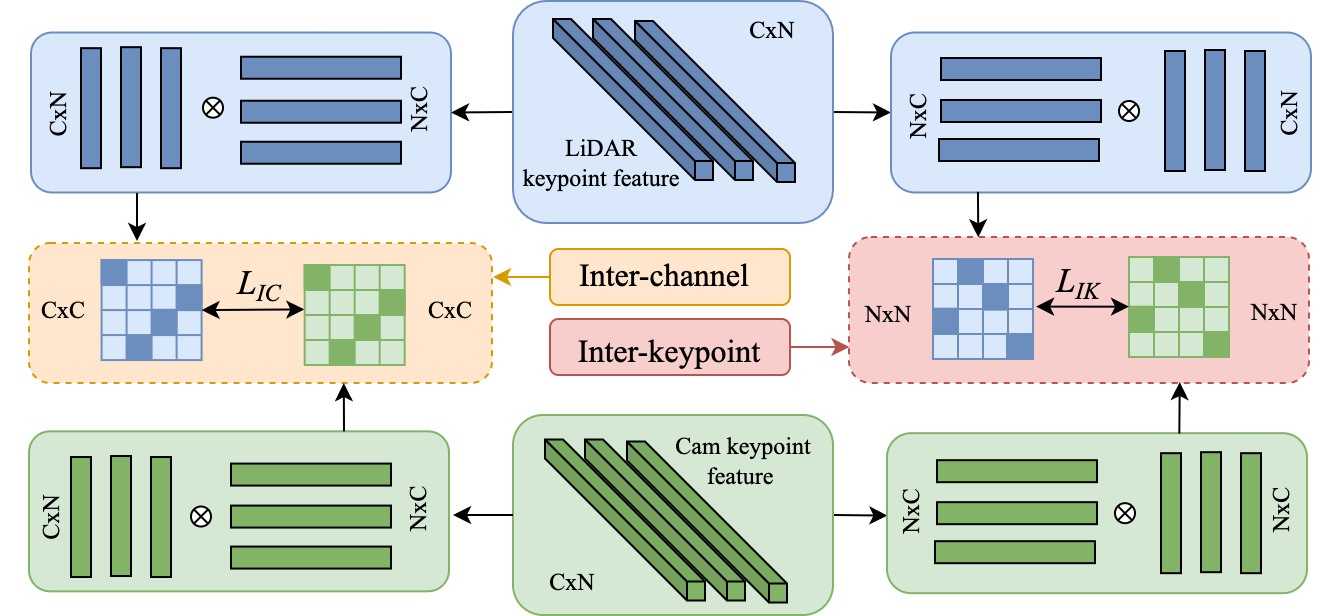
\includegraphics[scale=0.17]{cvpr_2022/iccv_fig6_2.drawio.png}
    \caption{\textbf{Detials of Innter-feature BEV Distillation.} For each foreground area in BEV space, we represent rach target feature by a set of keypoints and conduct feature distillation in both inter-channel and inter-keypoint manners.
    }
    \label{fig:structure_attn}
    % \vspace{-0.8cm}
\end{figure}

% and the corresponding background regions and divide into small grids with spatial resolution of $G_i\times G_i \times G_i$, which can summarize each foreground area into the certain number of feature keypoints.  For the bird-view feature maps, we project the keypoint $p_i$ to the 2D bird-view coordinate system and utilize bilinear interpolation to obtain the features $f^{bev}_i$ from the bird-view feature maps. Hence, the roi feature can be represented as follow:

% \begin{equation}
%     {F_i^{ROI}} = {f^{bev}_1,...,f^{bev}_i,f^{bev}_n}, 
%  i=1,..N
% \end{equation}
% which have the strong capability of preserving 3D geometry information of the foreground scene and can also boost the marginal awareness performance of the certain target.

\paragraph{Inter-channel BEV Distillation.}
% \label{sec:seq}
Taking the $j$-th object target as an example, we first apply an inter-channel BEV distillation, which guides the student keypoint features to mimic the channel-wise relationships of the teacher's. Such inter-channel signals imply the overall geometric semantics of each object target. Compared with the previous channel-by-channel supervision, our inter-channel distillation can preserve the distinctive aspects of the two modalities, while effectively transfer the well pre-trained knowledge of LiDAR-based detectors. Specifically, we calculate the inter-channel similarities of both camera-based and LiDAR-based keypoint features, formulated as
\begin{equation}
    A_j^{2d} = f_j^{2d} {f_j^{2d}}^{\top};\ \ \ A_j^{3d} = f_j^{3d} {f_j^{3d}}^{\top},
\end{equation}
where $A_j^{2d}, A_j^{3d} \in {\mathbb{R}^{C\times C}}$ denote the feature relationships between different $C$ channels for the two modalities. For all $M$ objects in a scene, we adopt L2 loss between the two inter-channel similarities for feature distillation, formulated as
\begin{equation}
    \mathcal{L}_{\rm{bev}}^{{IC}}= \sum_{j=1}^{M} ||A_j^{3d}-A_j^{2d}||_2.
    \label{eq:fm}
\end{equation}

% Given the RoI feature of each box proposal, the lidar-based bev feature and cam-based bev feature can be represented as $F_i^{Lidar}\in {\mathbb{R}^{N\times C}}$, $F_i^{cam}\in {\mathbb{R}^{N\times C}}$ respectively, where ${N}$ represents the number of keypoints and ${C}$ represents the channels numbers. For the certain sampled feature of the keypoint, it reflects the certain information within the receptive field. As mentioned before, the lidar-based detector has the better detection performance since the spatial information of the same inner roi location contains the richer semantic information compare to the cam-based detector. Thus, we propose a inner target-aware (\textbf{ITA}) distillation that performs distillation within channel wise, which allows student to learn the context of feature from RoI patches and retain the correlation among different channels. For the bev feature ${i}$th ROI, the channel-wise information matrix is defined as: 
% \begin{equation}
%     {G_i^{ROI}} = {F^{Lidar}_i\cdot {F^{Lidar}_i}}^{\top}
% \end{equation}
% The information matrix has a size of ${C\times C}$ regardless of the spatial dimension ${N}$. ${G_{i,(m,n)}^{ROI}}$ denotes the inner channel correlation between $m$th channel and $n$th channel for the same location of the $i$th ROI.

% \begin{equation}
% \begin{aligned}
% %L_{task} = &\lambda_1 L_{per}(G_s(x),G_t(x))  +\lambda_1  L_{CE}(y,\delta(z_s))\\ & + \lambda_1L_{Focal}(y,y_{out})
% %{G_{i,(m,n)}^{ROI}} = &{f^_{1,m}}{f^_{1,n}}^{\top}  +{f^_{2,m}}{f^_{2,n}}^{\top} + \dots + \\&{f^_{N,m}}\cdot {f^_{N,n}}^{\top}
% {G_{i,(m,n)}^{ROI}} = &{f^_{1,m}}\cdot {f^_{1,n}}^{\top} + {f^_{2,m}}\cdot {f^_{2,n}}^{\top}\\ & + \dots + \\{f^_{N,m}}\cdot {f^_{N,n}}^{\top}
% \end{aligned}
% \end{equation}


% For the same roi area, to make the whole cam-based detector mimic
% a spatial component of the lidar-based detector, we use the Inner-target aware operator ${G_{i,(m,n)}^{ROI}}$ to pixel-wisely reconfigure the
% semantic of cam-based feature in the certain position and transfer the channel correlation of the lidar-based feature to the cam-based feature in the certain position. Conditioned on the same roi, the ${G_{i,(m,n)}^{ROI}}$ should reflect the semantic similarity with between the components. 

% We penalize the $L_2$ distance between the channel-wise information matrix of the lidar-based detector and the cam-based detector, allowing the cam-based to obtain the similar feature diversity for the same foreground area.
% \begin{equation}
%     \mathcal{L}_{\rm{ITA}}= ||G^{Lidar}_{i,cha}-G^{cam}_{i,cha}||_2.
%     \label{eq:fm}
% \end{equation}


\begin{table*}[ht]
\centering
\caption{\textbf{Performance Comparison on nuScenes~\cite{b6} Val Set.} 'C' and 'L' denote the camera-based and LiDAR-based methods, which refer to the input data during inference. * denotes our implementation using BEVDet\cite{b19} codebase.
%using their official codes.
% We have at least 1 absolute point of performance gain against KD \cite{Hinton2015DistillingTK} on 5 out of 7 experimental settings.
}
%\vspace{-0.2cm}
\resizebox{2\columnwidth}{!}{
\tablestyle{5pt}{1.2}
\begin{tabular}{c|c|c|c|cc|ccccc}
\toprule[1.2pt]
Method          & Modality & Backbone & Resolution & mAP↑  &NDS↑& mATE↓ & mASE↓ & mAOE↓ & mAVE↓ & mAAE↓   \\ \midrule
FCOS3D\cite{b12}          & C  &ResNet-101 & 900 $\times$ 1600 & 0.343& 0.415 & 0.725 & 0.263 & 0.422 & 1.292 & 0.153  \\
PGD\cite{b17}             & C  &ResNet-101 & 900 $\times$ 1600 & 0.369& 0.428 & 0.683 & 0.260 & 0.439 & 1.268 & 0.185  \\
MonoDETR\cite{b47}             & C  &ResNet-101 & 900 $\times$ 1600 & 0.372& 0.434 & 0.676 & 0.258 & 0.429 & 1.253 & 0.176  \\
%BEVDepth-R50        & C &ResNet-50   & 256 \times 704  & 0.351 & 0.639 & 0.267 & 0.479 & 0.428 & 0.198 & 0.475 \\
% BEVDepth\cite{b7}         & C &ResNet-101  & 512 \times 1408 & 0.412 & 0.565 & 0.266 & 0.358 & 0.331 & 0.190 & 0.535 \\
DETR3D\cite{b13}          & C &ResNet-101  & 900 $\times$ 1600 & 0.303& 0.374 & 0.860 & 0.278 & 0.437 & 0.967 & 0.235  \\
PETR\cite{b21}            & C  &ResNet-101    & 512 $\times$ 1408 & 0.357 & 0.421& 0.710 & 0.270 & 0.490 & 0.885 & 0.224  \\
BEVFormer\cite{b11}       & C  &ResNet-101   & 900 $\times$ 1600 & 0.416 & 0.517& 0.673 & 0.274 & 0.372 & 0.394 & 0.198   \\
PETRv2\cite{b24}            & C  &ResNet-101    & 640 $\times$ 1600 & 0.421& 0.524 & 0.681 & 0.267 & 0.357 & 0.377 & 0.186  \\
MonoDETR-MV\cite{b48}            & C  &ResNet-101    & 640 $\times$ 1600 & 0.428 & 0.531 & 0.676 & 0.268 & 0.352 & 0.380 & 0.169  \\ \midrule
CenterPoint~\cite{b53} (Teacher)   & L &VoxelNet   & -          & 0.564 & 0.646& 0.299 & 0.254 & 0.330 & 0.286 & 0.191  \\ \midrule
BEVDet$^*$ \cite{b19} & C &ResNet-50   & 256 $\times$ 704 & 0.298& 0.379 & 0.725 & 0.279 & 0.589 & 0.860 & 0.245  \\ 
\rowcolor{gray!12} \textbf{+ TiG-BEV}     &C  &ResNet-50  & 256 $\times$ 704 & \textbf{0.331} & \textbf{0.411}& 0.678 & 0.271 & 0.589 & 0.784 & 0.218  \\ 
\rowcolor{gray!12}& &&& \textbf{\textcolor{blue}{+3.3$\%$} }& \textbf{\textcolor{blue}{+3.2$\%$}}&\textcolor{blue}{-4.7$\%$} & \textcolor{blue}{-0.8$\%$} & \textcolor{blue}{-0.0$\%$} & \textcolor{blue}{-7.6$\%$} & \textcolor{blue}{-2.7$\%$}   \\ 
\midrule
BEVDet4D$^*$ \cite{b23} & C &ResNet-50   & 256 $\times$ 704 & 0.322 & 0.451& 0.724& 0.277& 0.520 &0.366 &0.212  \\
\rowcolor{gray!12} \textbf{+ TiG-BEV}     & C &ResNet-50  & 256 $\times$ 704 & \textbf{0.356}& \textbf{0.477} & 0.648 & 0.273 & 0.517 & 0.364 & 0.210  \\ 
\rowcolor{gray!12}& &&& \textbf{\textcolor{blue}{+3.4$\%$} }& \textbf{\textcolor{blue}{+2.6$\%$}}&\textcolor{blue}{-7.6$\%$} & \textcolor{blue}{-0.4$\%$} & \textcolor{blue}{-0.3$\%$} & \textcolor{blue}{-0.2$\%$} & \textcolor{blue}{-0.2$\%$}   \\ 
\midrule
BEVDepth$^*$ \cite{b7} & C &ResNet-101   & 512 $\times$ 1408 & 0.416 & 0.521& 0.605 & 0.268 & 0.455 & 0.333 & 0.203  \\
\rowcolor{gray!12}   \textbf{+ TiG-BEV}   & C & ResNet-101  & 512 $\times$ 1408  & \textbf{0.440}& \textbf{0.544} & 0.570 & 0.267 & 0.392 & 0.331 & 0.201  \\ 
\rowcolor{gray!12}& &&& \textbf{\textcolor{blue}{+2.4$\%$} }& \textbf{\textcolor{blue}{+2.3$\%$}}&\textcolor{blue}{-3.5$\%$} & \textcolor{blue}{-0.1$\%$} & \textcolor{blue}{-6.3$\%$} & \textcolor{blue}{-0.2$\%$} & \textcolor{blue}{-0.2$\%$}   \\ 
\bottomrule[1.2pt]
\end{tabular}
}

\label{tab:nus_val_sota}
%\vspace{-3mm}
\end{table*}
\paragraph{Inter-keypoint BEV Distillation.}
\label{sec:anchor}
The inter-channel distillation guides the camera-based detector to learn the channel-wise diversity from the LiDAR-based teacher. However, it is conducted without considering the inner correlation of different keypoints within each object target, which is not capable of capturing the local geometries among different foreground parts, e.g., the front and rear of cars. To this end, we propose to utilize the inter-keypoint correlations of LiDAR-based BEV features and transfer such inner-geometry semantics into camera-based detectors. Analogous to the aforementioned inter-channel module, for the $j$-th target object, we calculate the inter-keypoint similarities in a transposed manner for the two modalities as
\begin{equation}
    B_j^{2d} = {f_j^{2d}}^{\top} {f_j^{2d}};\ \ \ B_j^{3d} = {f_j^{3d}}^{\top} {f_j^{3d}},
\end{equation}
where $B_j^{2d}, B_j^{3d} \in {\mathbb{R}^{N\times N}}$ denote the feature relationships between different $N$ keypoints respectively for camera and LiDAR. We also adopt L2 loss for all $M$ targets as
\begin{equation}
    \mathcal{L}_{\rm{bev}}^{{IK}}= \sum_{j=1}^{M} ||B_j^{3d}-B_j^{2d}||_2.
    \label{eq:fm}
\end{equation}
Then, the distillation loss for inter-channel and inter-keypoint features in BEV space is formulated as
\begin{equation}
    \mathcal{L}_{\rm{bev}}=
    \mathcal{L}_{\rm{bev}}^{{IC}}+
    \mathcal{L}_{\rm{bev}}^{{IK}},
    \label{eq:seg}
\end{equation}
where the two terms are orthogonal respectively for the channel-wise feature diversity and keypoint-wise semantic correlations.

% The attempt to preserve the local correlation through concatenating all the position would fail. 
% We hope that detector can capture the context from the one position to another within the target area. In this case, the cam-based detector will, however, be distracted from the locality since the \textbf{ITA} encodes all the related semantic over the whole feature among different positions. In other words, the \textbf{ITA} will aggregates redundant local semantic.
% Furthermore, a large feature map will hinder the inductive bias since it may encourage the student to integrate the less relevant semantic from remote positions by mistake, which may deteriorate the subsequent distillation performance.
% For complex scenes and similar targets, the postion wise dependency is important to capture the relation (\eg layout) of different components within the target.

% We address the conundrum by the proposed local target-aware(\textbf{LTA}) distillation. Like the the channel-wise information matrix defined in \textbf{ITA}, the position-wise matrix is defined as follow:
% \begin{equation}
%     {G_{i}^{pos}} = {{F^{Lidar}_i}^{\top}\cdot F^{Lidar}_i}
% \end{equation}

% The information matrix has the size of ${N\times N}$ regardless of the channel dimension ${C}$. ${G_{i,(p,q)}^{pos}}$ denotes the inner spatial correlation between $p$th keypoint and $q$th keypoint for the $i$th ROI. Similarly, the formulation of the operator can be defined as:

% \begin{equation}
% \begin{aligned}
%     {G_{i,(p,q)}^{pos}} = {f^_{p,1}}\cdot {f^_{q,1}}^{\top} + {f^_{p,2}}\cdot {f^_{q,2}}^{\top} + \dots + \\{f^_{p,C}}\cdot {f^_{q,C}}^{\top}
% \end{aligned}
% \end{equation}

% After reconfiguration, the spatial relationship within the target can be extracted and summerized, which is complementary to the channel relationship. Therefore, as the cam-based detector, we enhance its gemetry expressivity by asking them to mimic the teacher. Thus, the objective for (\textbf{LTA}) knowledge distillation can be given by:

% \begin{equation}
%     \mathcal{L}_{\rm{LTA}}= ||G^{Lidar}_{i, pos}-G^{Cam}_{i, pos}||_2.
%     \label{eq:fm}
% \end{equation}

\subsection{Overall Loss}
\label{sec:overall_loss}
To sum up, we benefit the student camera-based detector by target inner-geometry from two complementary aspects, i.e., an inner-depth supervision for low-level signals and an inner-feature BEV distillation for high-level semantics. They produce two losses as $\mathcal{L}^R_{\rm{depth}}$ and $\mathcal{L}_{\rm{bev}}$. Together with the original two losses, i.e., dense absolute depth supervision $\mathcal{L}^A_{\rm{depth}}$, and 3D detection $\mathcal{L}_{\rm{det}}$, the overall loss of our TiG-BEV is formulated as
\begin{equation}
    \mathcal{L}_{\rm{TiG}}=
    \mathcal{L}_{\rm{det}}+
    \mathcal{L}^A_{\rm{depth}}+
    \mathcal{L}^R_{\rm{depth}}+
    \mathcal{L}^{IC}_{\rm{bev}}+
    \mathcal{L}^{IK}_{\rm{bev}}.
    \label{eq:seg}
\end{equation}

% The inner target-aware distillation enables the detector to mimic the inner feature diversity while the local target-aware distillation allows it to learn the local representation over the spatial feature, which are complementary to each other. Therefore, the combination of these two objectives can bring the best of two worlds. Our objective designed for structured attention feature supervision can be written by:
% \begin{equation}
%     \mathcal{L}_{\rm{SAF}}=
%     \delta\mathcal{L}_{\rm{ITA}}+
%     \zeta\mathcal{L}_{\rm{LTA}}
%     \label{eq:seg}
% \end{equation}



% Finally, the total loss of our proposed method can be defined by:
% \begin{equation}
%     \mathcal{L}_{\rm{TiG}}=
%     \mathcal{L}_{\rm{det}}+
%     \mathcal{L}^A_{\rm{depth}}+
%     \mathcal{L}^R_{\rm{depth}}+
%     \mathcal{L}^{IC}_{\rm{bev}}+
%     \mathcal{L}^{IK}_{\rm{bev}}
%     \label{eq:seg}
% \end{equation}
% Here $L_{task}$ is the loss of the 3D detection task. $\alpha$, $\beta$, $\gamma$, $\delta$ and $\zeta$ are the weight factors to balance the loss.


\vspace{-0.2cm}
\section{Experiment}\label{sec:exp}
\vspace{-0.2cm}
In this section, we present the experimental results to validate the effectiveness of the proposed BAT algorithm on benchmark datasets and compare it with state-of-the-art baseline methods. We also verify that both two components are helpful and necessary for BAT. The implementation of the BAT can be found via \url{https://anonymous.4open.science/r/benign-adv-77C5}.

\vspace{-0.2cm}
\subsection{Experimental Setup}
\vspace{-0.1cm}
%\jt{we can put baselines here.} \\
%\jt{implementation details, such as optimization method}
In this work, in order to demonstrate the 
merit of BAT, we conduct the experiments mainly on benchmark datasets CIFAR100~\cite{krizhevsky2009learning} and Tiny~ImageNet~\cite{le2015tiny}, which are relatively complex datasets (i.e., containing larger fractions of atypical samples). For both datasets, we study the algorithms under the model architectures ResNet and WideResNet (WRN)~\cite{he2016deep}. In this section, we only present the results of ResNet18 for CIFAR100 and ResNet32 for Tiny~ImageNet and leave the results on WRN in Appendix~\ref{app:exp}. As a fair comparison with BAT, we implement the baseline algorithms including PGD adversarial training~\cite{madry2017towards} as well as its most popular variant TRADES~\cite{zhang2019theoretically}. In addition, we include several recent algorithms: MART~\cite{wang2019improving} and GAIRAT~\cite{zhang2020geometry}, which also incorporate reweighting strategies into adversarial training. For BAT and all baseline methods, we run the algorithms using SGD~\cite{bottou2010large} for 160 epochs with the learning rate that starts from 0.1 and decays by 0.1 after the epoch 80 and 120. More implementation details can be found in Appendix~\ref{app:exp}.

\textbf{Performance on CIFAR100.} For a comprehensive comparison between different methods on CIFAR100, in the results from Table~\ref{Tab:results_cifar100}, we report the models' clean accuracy and adversarial accuracy against $l_\infty$-$8/255$ PGD attack~\cite{madry2017towards}, as well as their performance on the typical sample set and atypical sample set (as described in Section~\ref{sec:pre}). A more comprehensive robustness evaluation on different attacking methods (including CW~\cite{carlini2017towards} and Auto-Attack~\cite{croce2020reliable}) are presented in Appendix~\ref{app:exp}. For BAT, we report its performance when choosing its optimal hyperparameter: $\alpha = 1  ~\text{\&} ~2$ and $\beta = 0.2$. In the Section~\ref{sec:ablation}, we will discuss the impact of the selection of $\alpha$ and $\beta$ on BAT. For baseline methods, the settings and checkpoint selections follow the original papers' suggestions.

%Note that the main goal of BAT is not to improve model's adversarial robustness, so we leave the robustness evaluation with additional attacking methods, such as CW~\cite{carlini2017towards} and Auto Attack~\cite{croce2020reliable} in  Appendix~\ref{app:exp} where we have similar observations.

\vspace{-0.3cm}
\begin{table}[h]
\small
\centering
\caption{Performance of BAT vs. Baselines on CIFAR100 Under ResNet18}
\begin{tabular}{c|cc|cc|cc}
\hline
Method & All Acc. & All Adv. & Typical Acc. & Typical Adv. & Atyp. Acc. & Atyp. Adv. \\
\hline
\hline
PGD Train (Best Adv.) & 56.9 & 27.4 & 90.6 & 59.0 &29.5 & 7.7\\
PGD Train (Best Clean) & 57.8 & 21.9 & 88.3 & 51.0 & \textbf{40.1} & 8.3 \\
%TRADES ($1/\lambda = 1$) & \textbf{61.3} & 21.9 & \textbf{93.0} & 50.0 & 44.7 & 7.9\\
TRADES ($1/\lambda = 5$) & 56.6 & 26.9 & 88.9 & 57.1 & 37.3 & \textbf{10.9} \\
MART~\cite{wang2019improving} & 51.8 & \textbf{30.4} & 85.3 & \textbf{62.2} & 25.3 & 10.1\\
GAIRAT~\cite{zhang2020geometry} & 58.2 & 27.8 & 90.6 & 60.7 & 31.6 & 8.2\\
\hline
BAT ($\alpha = 1, \beta = 0.2$) & \textbf{59.5} &27.3 & \textbf{92.3} & 58.8 & 36.3 & 8.7 \\
BAT ($\alpha = 2, \beta = 0.2$) &59.3 & 27.4 & \textbf{92.3} & 60.3 & 33.1 & 7.4 \\
\hline
\hline
\end{tabular}
\label{Tab:results_cifar100}
\end{table}
\vspace{-0.2cm}
From the results in Table~\ref{Tab:results_cifar100}, we can find that BATs enjoy good clean \& adversarial accuracy trade-off among all methods. It is because BATs can obtain the highest overall clean accuracy ($\sim59.5\%$), as well as comparably good adversarial accuracy ($\sim27.3$) with baseline methods. The only exception is MART~\cite{wang2019improving} which has the higher adversarial accuracy around $\sim 30\%$. However, MART~\cite{wang2019improving} has much lower clean accuracy than BATs. 

To gain a deeper understanding of the working mechanism of BAT, we focus on the performance on BAT vs. PGD adversarial training~\cite{madry2017towards}. Compared with PGD adversarial training with highest adversarial accuracy (PGD Train (Best Adv.)), the BAT methods are $2\sim3\%$ higher in terms of overall clean accuracy, and similar adversarial accuracy. The improvement of clean accuracy is mainly due to BATs' capacity to fit much more atypical samples. For example, the clean accuracy of BAT ($\alpha=1, \beta=0.2$) is about $6\%$ higher than PGD Train~(Best Adv.). On the other hand, compared to PGD adversarial training with the highest clean accuracy (PGD Train (Best Clean)), BATs have much better overall adversarial robustness and slightly better clean accuracy. This is mainly due to BAT's advantage on typical samples, because BATs can successfully prevent the performance drop of typical samples during the training process. Since BATs can achieve good performance on both typical samples and atypical samples, BATs outperform PGD adversarial training in CIFAR100.

\begin{wrapfigure}{r}{0.6\textwidth}
\vspace{-0.4cm}
\subfloat{
\begin{minipage}[c]{0.3\textwidth}
\centering
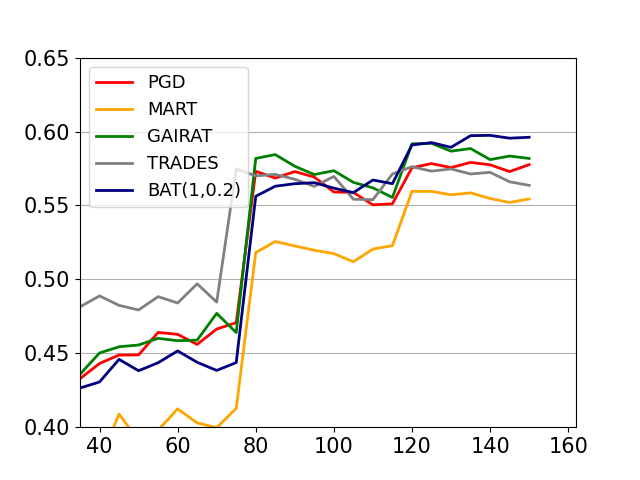
\includegraphics[width = 1.1\textwidth]{figures/base_clean.png}
\end{minipage}
}
\subfloat{
\begin{minipage}[c]{0.3\textwidth}
\centering
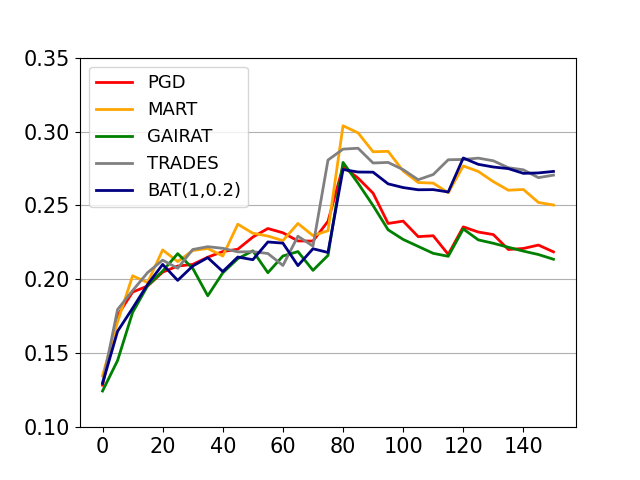
\includegraphics[width = 1.1\textwidth]{figures/base_rob.png}
\end{minipage}
}
\vspace{-0.4cm}
\caption{\small Clean Acc. (left) \& Adv. Acc (right)}
\label{fig:exp1}
\end{wrapfigure}
In Fig.~\ref{fig:exp1}, we also show the change of each models' overall clean accuracy (Fig~\ref{fig:exp1} (left)) \& adversarial accuracy (Fig~\ref{fig:exp1} (right)) along with the training progress. 
Interestingly, similar to PGD adversarial training, all baseline methods cannot achieve the optimal clean and adversarial accuracy at the same moment.
They always achieve the best adversarial accuracy around Epoch 80 (right after the first time weight decay), and the best clean accuracy on the last epochs. However, for BATs, since they can effectively prevent the robustness dropping in the late epochs, BATs are able to train until last epochs and enjoy good clean and adversarial accuracy simultaneously.
%As a result, BATs have higher clean accuracy than all baseline models, and good adversarial accuracy, which are similar or comparable to all baselines (even on their best checkpoints).

\textbf{Performance on Tiny~ImageNet.} Tiny~ImageNet~\cite{le2015tiny} contains 200 classes of the images in the original ImageNet~\cite{krizhevsky2012imagenet} dataset, with 500 training images for each class, and image size $64\times 64$. In our experiments, we only choose the first 50 classes in Tiny ImageNet for training and prediction. Since the image size is $64\times 64$, for both training and robustness evaluation, we consider the adversarial attacks are bounded by $l_\infty$-norm-4/255. In Table~\ref{Tab:results_imagenet}, we report the performance of BAT and baseline methods. Similar to the conclusions we can make from CIFAR100, BATs can achieve the highest overall clean accuracy and comparably good adversarial accuracy with baseline methods. 
\begin{table}[h]
\small
\vspace{-0.2cm}
\centering
\caption{Performance of BAT vs. Baselines on Tiny~ImageNet Under ResNet32}
\begin{tabular}{c|cc|cc|cc}
\hline
Method & All Acc. & All Adv. & Typical Acc. & Typical Adv. & Atyp. Acc. & Atyp. Adv. \\
\hline
\hline
Adv. Train (Best Adv.) & 56.3 & 32.3 & 97.5 & 85.3 &41.5 & 9.6\\
Adv. Train (Best Clean) & 58.2 & 30.5 & 98.0 & 80.4 & 44.7 & 9.1 \\
TRADES ($1/\lambda = 5$) & 55.4 & 28.8 & 97.3 & 77.4 & 38.8 & 9.6 \\
MART~\cite{wang2019improving} & 56.2 & \textbf{34.5} & 97.7 & 85.1 & 41.4 & \textbf{13.6} \\
GAIRAT~\cite{zhang2020geometry} & 58.4 & 30.4 & 98.0 & 81.7 & 45.7 & 7.8\\
\hline
BAT ($\alpha = 1, \beta = 0.2$) & \textbf{59.4} &32.0 & 98.4 & 83.9 & \textbf{48.4} & 10.2 \\
BAT ($\alpha = 2, \beta = 0.2$) &\textbf{59.4} &32.9 & \textbf{99.1} & \textbf{86.9} & 45.7 & 10.9 \\
\hline
\hline
\end{tabular}
\label{Tab:results_imagenet}
\end{table}

\vspace{-0.7cm}
\subsection{Ablation Study}\label{sec:ablation}
\vspace{-0.2cm}
\begin{wrapfigure}{r}{0.6\textwidth}
\vspace{-0.9cm}
\subfloat{
\begin{minipage}[c]{0.32\textwidth}
\centering
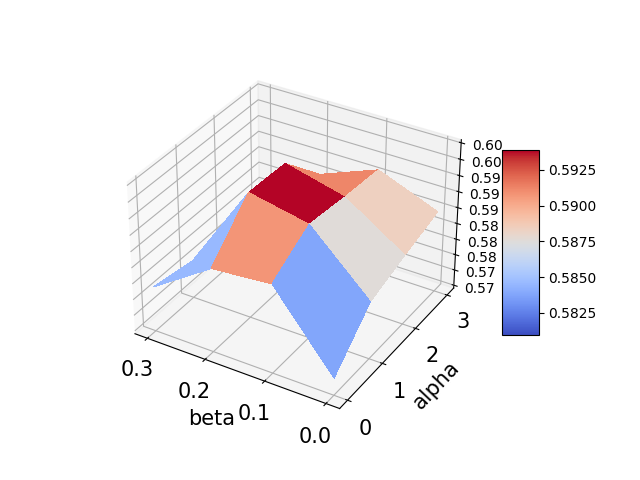
\includegraphics[width = 1.1\textwidth]{figures/abl_clean.png}
\end{minipage}
}
\subfloat{
\begin{minipage}[c]{0.32\textwidth}
\centering
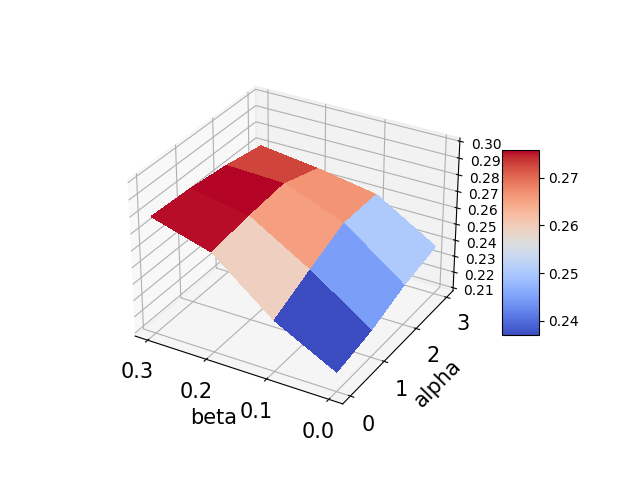
\includegraphics[width = 1.1\textwidth]{figures/abl_rob.png}
\end{minipage}
}
\caption{\small Clean Acc.(left) \& Adv. Acc.(right)}
\label{fig:exp2}
\vspace{-0.2cm}
\end{wrapfigure}
In this subsection, we study the potential impact of the hyperparameters chosen in BAT, which is $\alpha$ that controls the \textit{Reweighting} process and $\beta$ that controls the \textit{Discrimination Loss}. 
In Fig.~\ref{fig:exp2}, we conduct the experiments on CIFAR100 with BAT when $\alpha$ is chosen in [0,1,2,3] and $\beta$ is in [0, 0.1, 0.2, 0.3].
In Fig.~\ref{fig:exp2}, we show each model's overall clean accuracy~(left) \& adversarial accuracy~(right) along the Z-axis, and X-axis / Y-axis indicate the models' corresponding variables of $(\alpha,\beta)$. Note that when $\alpha=\beta=0$, the BAT method regresses to original PGD adversarial training. From the result, we can see that a positive pair of $(\alpha,\beta)$ can benefit both model clean and adversarial accuracy. Therefore, both two components \textit{Reweighting} and \textit{Discrimination Loss} of BAT are helpful and necessary. However, when $\alpha$ or $\beta$ is relatively too large, it will hurt the BAT's clean accuracy. As a result, in CIFAR~100, when $\alpha=1$ or 2 and $\beta= 0.2$, BAT can achieve the optimal performance.

%If we look at the performance of these models at their final epochs, we first observe that $\beta=0.2$ can improve both clean and adversarial accuracy, compared to all models with $\beta = 0$. Moreover, given any fixed value of $\beta$, the model with $\alpha = 1$ or 2 always outperforms than $\alpha=0$.
%Since a positive $\alpha$ indicates the BAT algorithm downweight or exclude certain samples during the training process, we can conclude that those  samples which are downweighted/excluded are acting like poisoning samples to deteriorate the models' performance. and necessary.

\vspace{-0.4cm}
\section{Related Works}
\vspace{-0.3cm}
\textbf{Memorization and atypical samples.} The memorization effect of overparameterized DNNs have been extensively studied both empirically~\cite{zhang2016understanding, nakkiran2019deep} and theoretically~\cite{bartlett2002rademacher}. From traditional views, the memorization can be harmful to the model generalization, because it makes DNN models easily fit those outliers and noisy labels.  However, recent studies point out the concept of ``benign overfitting''~\cite{bartlett2020benign, feldman2020does, feldman2020neural}, which suggests the memorization effect necessary for DNNs to have extraordinary performance on modern machine learning tasks. 
Especially, the recent work~\cite{feldman2020neural} empirically figures out those atypical/rare samples in benchmark datasets and show the contribution from memorizing atypical samples to the DNN's performance. Besides the work~\cite{feldman2020neural}, there are also other strategies~\cite{carlini2019distribution} to find atypical samples in training dataset.  Notably, our work is not the first effort to study the influence of memorization on DNN's adversarial robustness. A previous study~\cite{sanyal2020benign} illustrates that memorizing the mis-labeled samples might be a reason to cause the DNNs' adversarial vulnerability. In our paper, we focus on atypical samples, which appear much more frequently in common datasets, and we study their impacts especially on adversarial training algorithms~\cite{madry2017towards, zhang2019theoretically,chatterji2020finite, muthukumar2020harmless}.\\
\textbf{Adversarial robustness. } 
Adversarial training methods~\cite{madry2017towards, zhang2019theoretically, wang2019improving, zhang2016understanding, rice2020overfitting} are considered as one of the most reliable and effective methods to protect DNN models against adversarial attacks~\cite{goodfellow2014explaining, xu2019adversarial}. However, there are several intrinsic properties of adversarial training which requires deeper understandings. 
For example, they always suffer from poor robustness generalization~\cite{ schmidt2018adversarially, rice2020overfitting}, and they always present strong trade-off relation between clean accuracy vs. robustness~\cite{tsipras2018robustness, zhang2019theoretically}. Our work aims to study these properties from the data perspective and demonstrate the significant connection of the memorization effect with these properties.

\vspace{-0.4cm}
\section{Conclusion}
\vspace{-0.2cm}
In this paper, we draw significant connections of the memorization effect of deep neural networks with the behaviors of adversarial training algorithms. Based on the findings, we devise a novel algorithm BAT to enhance the performance of adversarial training. The findings of the paper can motivate the futures studies in building robust DNNs with more attention on the data perspective.
\bibliographystyle{unsrt}
\bibliography{sample}
%
%%%%%%%%%%%%%%%%%%%%%%%%%%%%%%%%%%%%%%%%%%%%%%%%%%%%%%%%%%%%
\section*{Checklist}

%%% BEGIN INSTRUCTIONS %%%
The checklist follows the references.  Please
read the checklist guidelines carefully for information on how to answer these
questions.  For each question, change the default \answerTODO{} to \answerYes{},
\answerNo{}, or \answerNA{}.  You are strongly encouraged to include a {\bf
justification to your answer}, either by referencing the appropriate section of
your paper or providing a brief inline description.  For example:
\begin{itemize}
  \item Did you include the license to the code and datasets? \answerYes{See Section.}
  \item Did you include the license to the code and datasets? \answerNo{The code and the data are proprietary.}
  \item Did you include the license to the code and datasets? \answerYes{}
\end{itemize}
Please do not modify the questions and only use the provided macros for your
answers.  Note that the Checklist section does not count towards the page
limit.  In your paper, please delete this instructions block and only keep the
Checklist section heading above along with the questions/answers below.
%%% END INSTRUCTIONS %%%

\begin{enumerate}

\item For all authors...
\begin{enumerate}
  \item Do the main claims made in the abstract and introduction accurately reflect the paper's contributions and scope?
    \answerYes{}
  \item Did you describe the limitations of your work?
    \answerYes{}
  \item Did you discuss any potential negative societal impacts of your work?
    \answerYes{}
  \item Have you read the ethics review guidelines and ensured that your paper conforms to them?
    \answerYes{}
\end{enumerate}

\item If you are including theoretical results...
\begin{enumerate}
  \item Did you state the full set of assumptions of all theoretical results?
    \answerYes{}
	\item Did you include complete proofs of all theoretical results?
    \answerYes{}
\end{enumerate}

\item If you ran experiments...
\begin{enumerate}
  \item Did you include the code, data, and instructions needed to reproduce the main experimental results (either in the supplemental material or as a URL)?
    \answerYes{} See Section~\ref{sec:exp}
  \item Did you specify all the training details (e.g., data splits, hyperparameters, how they were chosen)?
    \answerYes{} See Section~\ref{sec:exp}
    \item Did you report error bars (e.g., with respect to the random seed after running experiments multiple times)?
    \answerNo{}
	\item Did you include the total amount of compute and the type of resources used (e.g., type of GPUs, internal cluster, or cloud provider)?
    \answerYes{}
\end{enumerate}

\item If you are using existing assets (e.g., code, data, models) or curating/releasing new assets...
\begin{enumerate}
  \item If your work uses existing assets, did you cite the creators?
    \answerYes{}
  \item Did you mention the license of the assets?
    \answerYes{}
  \item Did you include any new assets either in the supplemental material or as a URL?
    \answerNo{}
  \item Did you discuss whether and how consent was obtained from people whose data you're using/curating?
    \answerNA{}
  \item Did you discuss whether the data you are using/curating contains personally identifiable information or offensive content?
    \answerNA{}
\end{enumerate}

\item If you used crowdsourcing or conducted research with human subjects...
\begin{enumerate}
  \item Did you include the full text of instructions given to participants and screenshots, if applicable?
    \answerNA{}
  \item Did you describe any potential participant risks, with links to Institutional Review Board (IRB) approvals, if applicable?
    \answerNA{}
  \item Did you include the estimated hourly wage paid to participants and the total amount spent on participant compensation?
    \answerNA{}
\end{enumerate}

\end{enumerate}




\appendix
\newpage
\begin{center}
% \large{\bf{Appendix for Graph Neural Networks}}
% \large{\bf{Supplementary Material}}
\large{\bf{Appendix}}
\end{center}

In the supplementary materials, we provide more details about atypical samples and the proposed algorithm, as well as the full experimental results of the preliminary study and the proposed method. 
\begin{itemize}
    \item Additional Introduction of Atypical Samples\hfill Appendix~\ref{app:atypical}
    \item Additional Results of Preliminary Study (in Section~\ref{sec:pre1})\hfill Appendix~\ref{app:pre1}
    \subitem Traditional ERM \& Adversarial Training
    \item Additional Results of Preliminary Study (in Section~\ref{sec:pre2})\hfill Appendix~\ref{app:pre2}
    \subitem Traditional ERM \& Adversarial Training
    \item Full Training Scheme of BAT\hfill Appendix~\ref{app:algorithm}
    \item Additional Results of BAT\hfill Appendix~\ref{app:exp}
    \item Boarder Impacts of this Paper \hfill Appendix~\ref{app:board}
\end{itemize}

\section{Additional Introduction of Atypical Samples}\label{app:atypical}

In this section, we provide additional introductions about the atypical samples in common datasets.
In Fig.~\ref{fig:show_mem}, we provide several examples of images from CIFAR10, CIFAR100~\cite{krizhevsky2009learning} and Tiny ImageNet~\cite{le2015tiny} respectively, with different memorization value (as defined in Section~\ref{sec:def_atypical}) around $0.0, 0.5, 1.0$. These examples suggest that if the memorization value of an image is large, this image is very likely to be ``atypical'', as it presents very distinct semantic features with the images in the main distribution (with memorization value 0.0). The detailed introduction about how to estimate the memorization value in practice can be found in the  work~\cite{feldman2020neural}.
\begin{figure}[h]
    \centering
    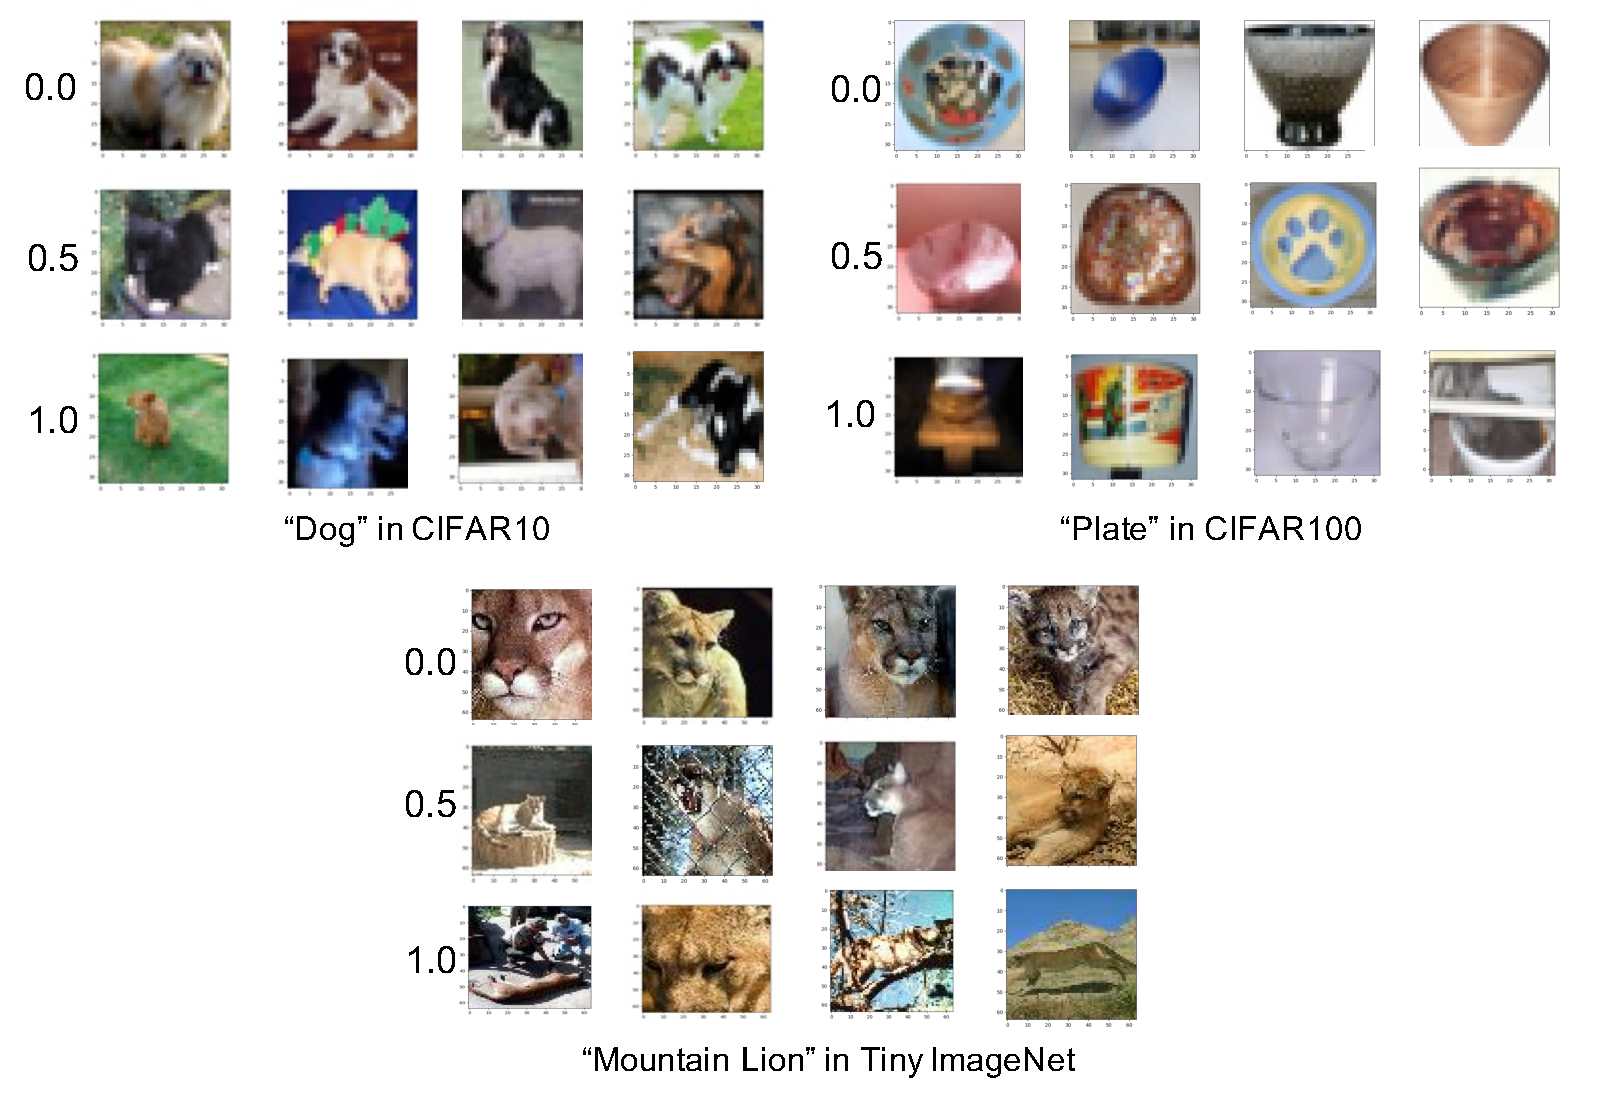
\includegraphics[width = 0.9\linewidth]{figures/atypical_examples.pdf}
    \caption{Examples of Images with Different Memorization Values}
    \label{fig:show_mem}
\end{figure}

\newpage
In Fig.~\ref{fig:hist}, we provide histograms to show the distribution of the estimated memorization values of all training samples from CIFAR10, CIFAR100 and Tiny~ImageNet. From Fig.~\ref{fig:hist}, we can observe that atypical samples (with high memorization value > 0.15) consist of a significant fraction (over 40\% \& 50\% respectively) in CIFAR100 and Tiny~ImageNet. In CIFAR10, they also consist of a non-ignorable fraction which is over 10\%.
\begin{figure}[h]
\centering
\subfloat[CIFAR100.]{
\begin{minipage}[c]{0.3\textwidth}
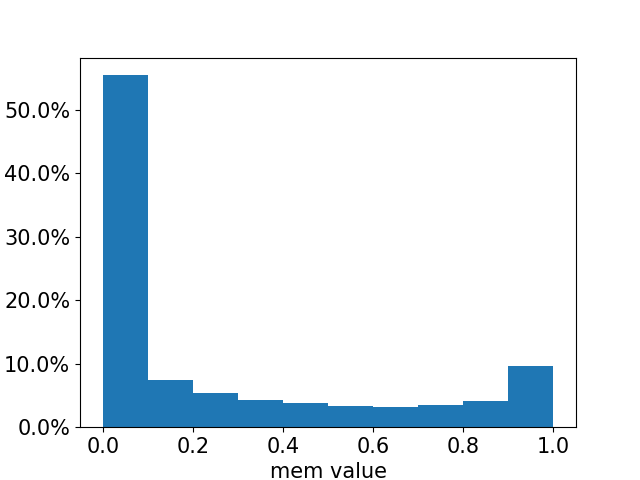
\includegraphics[width = 1.0\textwidth]{figures/hist_cifar100.png}
\end{minipage}
}
\hspace*{0.0cm}
\subfloat[CIFAR10.]{
\begin{minipage}[c]{0.3\textwidth}
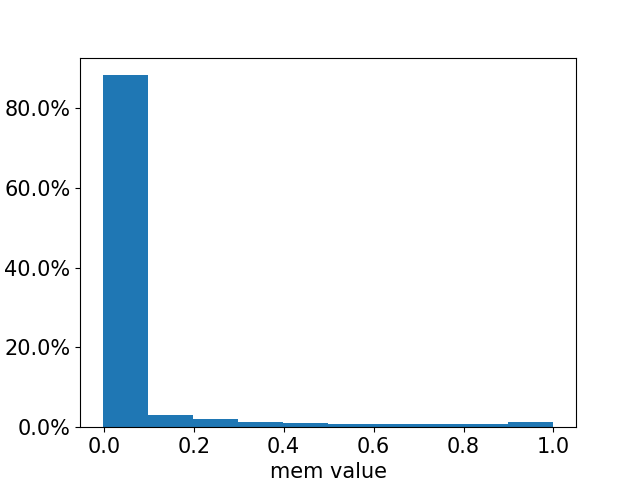
\includegraphics[width = 1.0\textwidth]{figures/hist_cifar10.png}%
\end{minipage}
}
\hspace*{0.0cm}
\subfloat[Tiny~ImageNet.]{
\begin{minipage}[c]{0.3\textwidth}
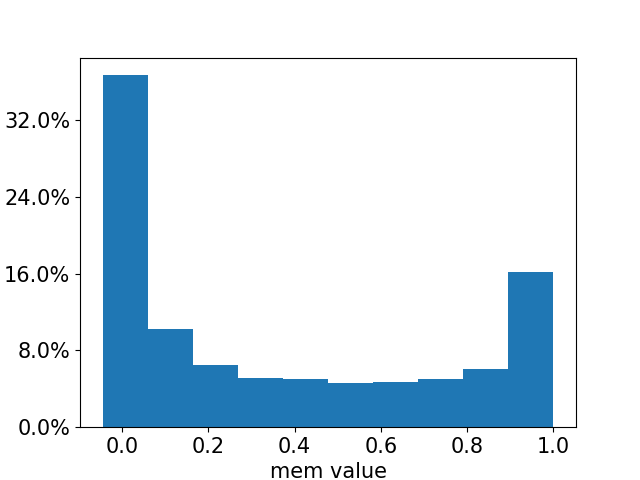
\includegraphics[width = 1.0\textwidth]{figures/hist_imagenet.png}%
\end{minipage}
}
\caption{Frequencies of Training samples with Different \textbf{Memorization Values} in Various Datasets}
\label{fig:hist}
\end{figure}


In Fig.~\ref{fig:show_pair}, we provide several pairs of images with high influence value (as defined in Section~\ref{sec:def_atypical}) which is over 0.15. In each pair, the training sample also has a high memorization value over 0.15. These examples suggest that there exist atypical samples in both training \& test sets of CIFAR10, CIFAR100 and Tiny~ImageNet. A pair of atypical samples (in the training set and test set) with a high influence value are visually very similar. Moreover, since they have high influence values, removing the atypical samples in the training set is very likely to cause the model to fail on the test atypical samples. Therefore, without memorizing the atypical sample in the training set, the model can hardly predict the atypical samples in the test set.
\begin{figure}[h]
    \centering
    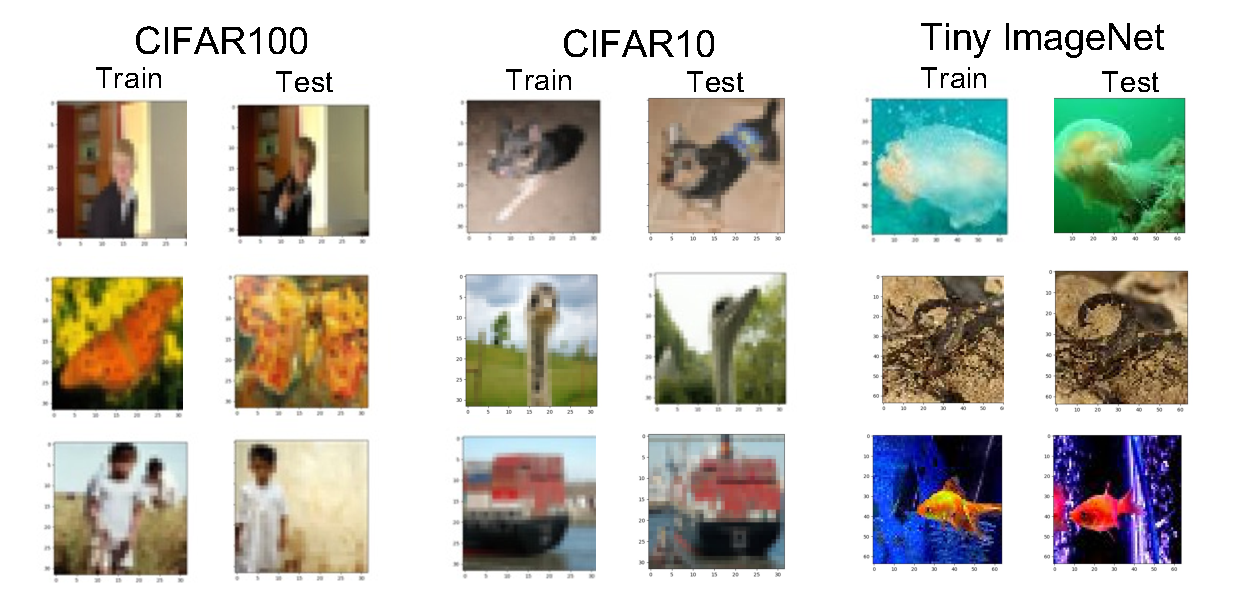
\includegraphics[width = 0.75\linewidth]{figures/pair.pdf}
    \caption{High Influence Pairs with Influence Value > 0.15}
    \label{fig:show_pair}
\end{figure}






\section{Additional Results for Preliminary Study}\label{app:pre}

In this section, we provide the full results of the preliminary study in Section~\ref{sec:pre} 
on CIFAR10, CIFAR100 and Tiny~ImageNet, to illustrate the distinct behaviors of the memorization effect between traditional ERMs and adversarial training. In both ERM and adversarial training, we train the models under ResNet18 and WideResNet28-10 (WRN28) architectures. In the experiments, we train the models for 200 epochs with learning rate 0.1, momentum 0.9, weight decay 5e-4, and decay the learning rate by 0.1 at the epoch 150 and 200. For adversarial training, we conduct experiments using PGD adversarial training~\cite{madry2017towards} by default to defense against $l_\infty$-8/255 adversarial attack, with the exception on Tiny~ImageNet, which is against $l_\infty$-4/255 attack. For robustness evaluation, we conduct a 20-step PGD attack.


\subsection{Additional Results for Preliminary Study - Section~\ref{sec:pre1}}\label{app:pre1}

In this subsection, we provide more experimental results to validate the statement 
in Section~\ref{sec:pre1}, where we state that fitting atypical samples in adversarial training can only improve the clean accuracy of test atypical samples, but hardly help their adversarial robustness. We provide full empirical results to show that: \textbf{(i)} In traditional ERM, fitting atypical samples improves the clean accuracy of test atypical samples. \textbf{(ii)} In adversarial training, fitting (adversarial) atypical samples improves the clean accuracy of test atypical samples but can hardly improve the adversarial robustness of them. The experimental setting follows Section~\ref{sec:pre1}, where we apply traditional ERM and adversarial training on original CIFAR10, CIFAR100, Tiny~ImageNet datasets. We evaluate the model's clean accuracy and adversarial accuracy on training atypical set $\mathcal{D}_\text{atyp}=\{x_i \in \mathcal{D}: \text{mem}(x_i)> 0.15\}$ and its corresponding test atypical set $\mathcal{D}_\text{atyp}' = \{x'_j \in \mathcal{D}': \text{infl}(x_i,x'_j)> 0.15, \text{for } \forall x_i\in \mathcal{D}_\text{atyp}\}$.


\textbf{(i) Additional Results for Preliminary Study - Section~\ref{sec:pre1} In Traditional ERM}

Fig.~\ref{fig:app_1_11}, Fig.~\ref{fig:app_1_12} and Fig.~\ref{fig:app_1_13} report the performance (clean accuracy) of traditional ERM, which is evaluated on atypical sets under ResNet18 (left) and WRN28 (right) on CIFAR100, CIFAR10 and Tiny~ImageNet. From the figures, we can obverse that fitting atypical samples during training can effectively help the models to achieve good clean accuracy on test atypical samples in all datasets. Note that here we only report clean accuracy as they are not robust against adversarial attacks.

\begin{figure}[h]
\centering
\hspace*{-1cm}
\subfloat[ResNet18.]{
\begin{minipage}[c]{0.3\textwidth}
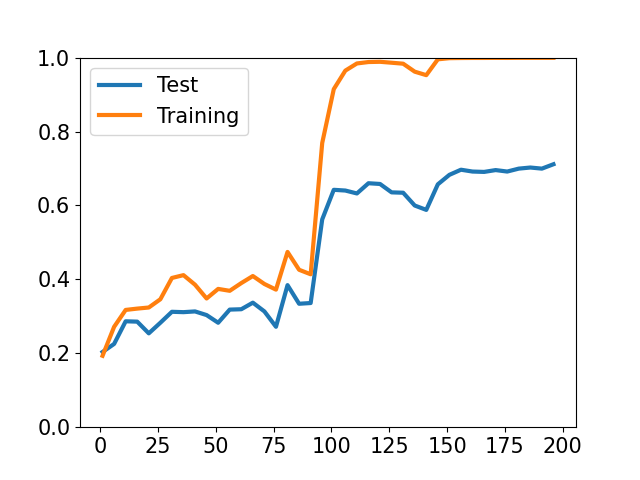
\includegraphics[width = 1.0\textwidth]{figures/pre1_clean_cifar100_ResNet18.png}
\end{minipage}
}
\hspace*{0.4cm}
\subfloat[ WRN28.]{
\begin{minipage}[c]{0.3\textwidth}
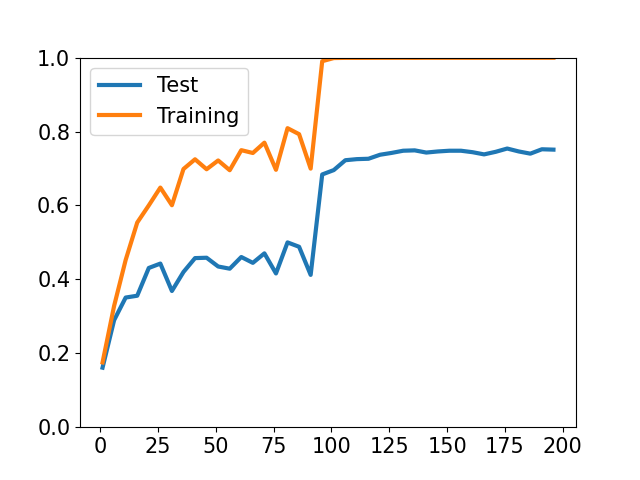
\includegraphics[width = 1.0\textwidth]{figures/pre1_clean_cifar100_WRN28.png}%
\end{minipage}
}
\caption{Clean Accuracy on \textbf{Atypical} Set of CIFAR100}
\label{fig:app_1_11}
\vspace{-0.5cm}
\end{figure}

\begin{figure}[h]
\centering
\hspace*{-1cm}
\subfloat[ ResNet18.]{
\begin{minipage}[c]{0.3\textwidth}
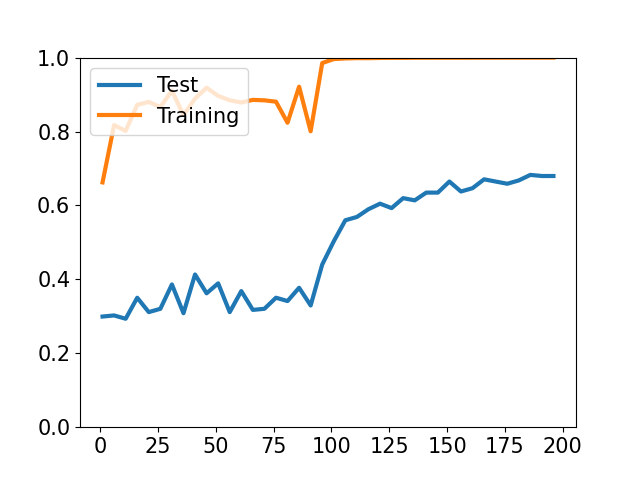
\includegraphics[width = 1.0\textwidth]{figures/pre1_clean_cifar10_ResNet18.png}
\end{minipage}
}
\hspace*{0.4cm}
\subfloat[WRN28.]{
\begin{minipage}[c]{0.3\textwidth}
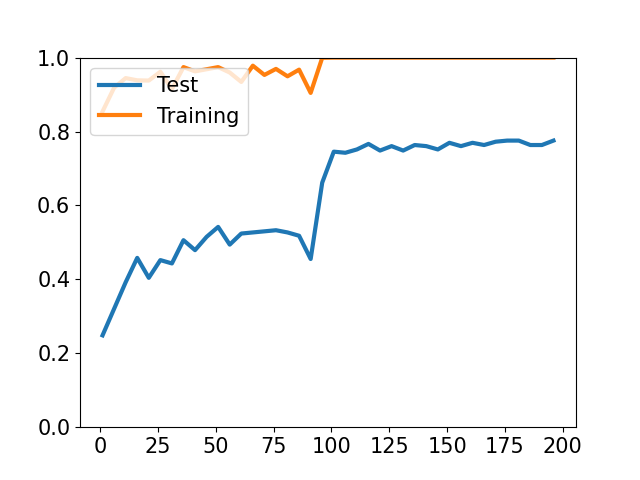
\includegraphics[width = 1.0\textwidth]{figures/pre1_clean_cifar10_WRN28.png}%
\end{minipage}
}
\caption{Clean Accuracy on \textbf{Atypical} Set of CIFAR10}
\label{fig:app_1_12}
\vspace{-0.5cm}
\end{figure}

\begin{figure}[h!]
\centering
\hspace*{-1cm}
\subfloat[ResNet32.]{
\begin{minipage}[c]{0.3\textwidth}
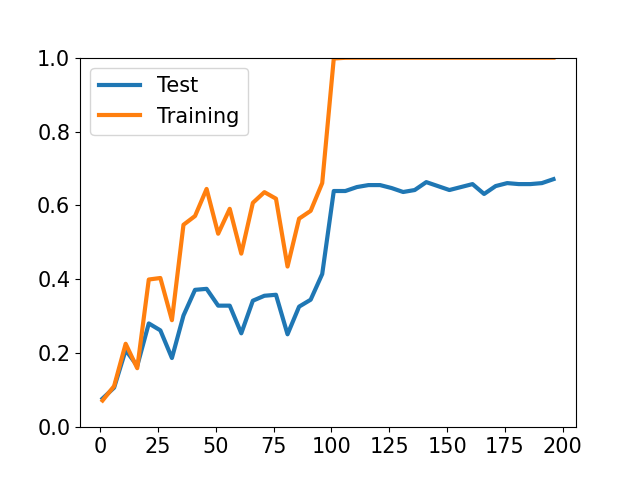
\includegraphics[width = 1.0\textwidth]{figures/pre1_clean_imagenet_ResNet18.png}
\end{minipage}
}
\hspace*{0.4cm}
\subfloat[WRN28.]{
\begin{minipage}[c]{0.3\textwidth}
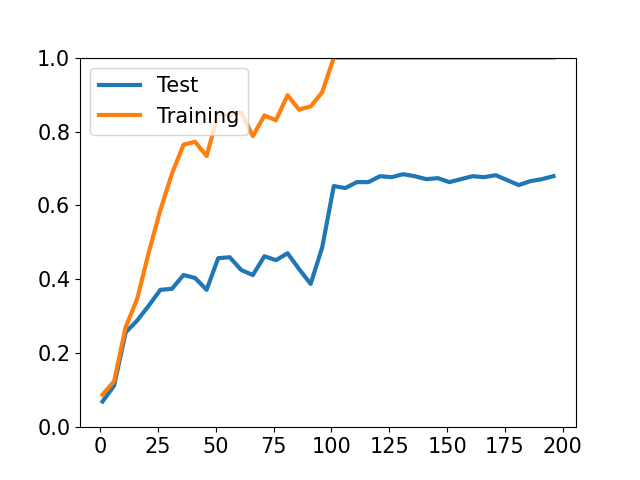
\includegraphics[width = 1.0\textwidth]{figures/pre1_clean_imagenet_WRN28.png}%
\end{minipage}
}
\caption{Clean Accuracy on \textbf{Atypical} Set of Tiny~ImageNet}
\label{fig:app_1_13}
\end{figure}

%%%%%%%%%%%%%%%%%%%%%%%%%%%%%%%%%%%%%%%%%%%%%%%%%%%%%%%%%%%%%%%%%%%%%%%%%%%%%%%%%%%%%%%%%%%%%%%%%%%%%%%%%%%%%%%%%%%%%%%%%%%%%%%%%%%%%%%%%%%%%%%%%%%%%%%%%%%%%%%%%%%%%%%%%%%%%%%%%%%%%%%%%%%%%%%%%%%%%%%%%%%%%%%%%%%%%%%%%%%%%%%%%%%%%%%%%%%%%%%%%%%%%%%%%%%%%%%%%%%%%%%%5

\newpage
\textbf{(ii) Additional Results for Preliminary Study - Section~\ref{sec:pre1} In Adversarial Training}

Fig.~\ref{fig:app_1_21}, Fig.~\ref{fig:app_1_22} and Fig.~\ref{fig:app_1_23} report the performance of adversarially trained models. We evaluate the clean accuracy and adversarial accuracy on the training atypical set $\mathcal{D}_\text{atyp}$ and test atypical set $\mathcal{D}'_\text{atyp}$. From the results, we can observe that although fitting atypical samples can help the model to have modest clean accuracy on test atypical samples, the adversarial robustness of them is constantly low and can hardly be improved during the whole training process.


\begin{figure}[h]
\centering
\hspace*{-1cm}
\subfloat[Clean (left) \& Adv Acc. (right) under ResNet18.]{
\begin{minipage}[h]{0.55\textwidth}
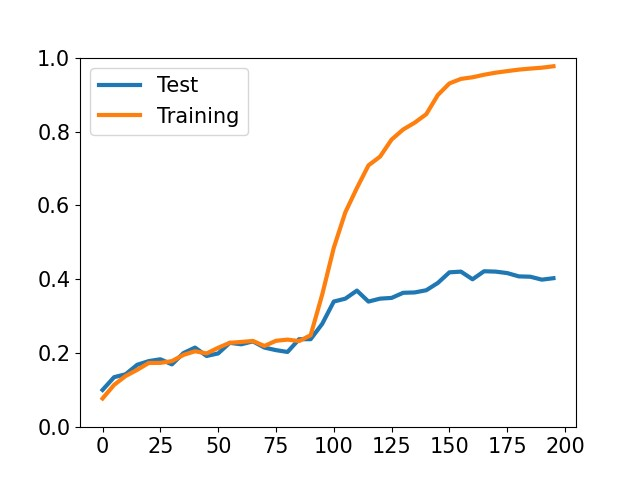
\includegraphics[width = 0.5\textwidth]{figures/clean_rare_cifar.jpg}%
\hfill
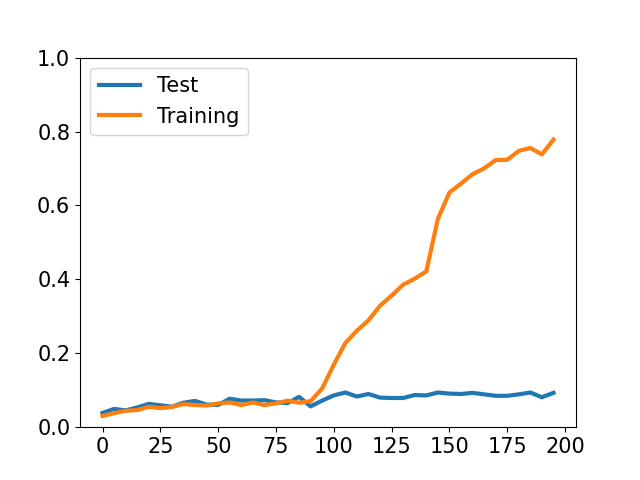
\includegraphics[width = 0.5\textwidth]{figures/adv_rare_cifar100.png}
\end{minipage}
}
\hspace*{-0.4cm}
\subfloat[Clean (left) \& Adv Acc. (right) under WRN28.]{
\begin{minipage}[c]{0.55\textwidth}
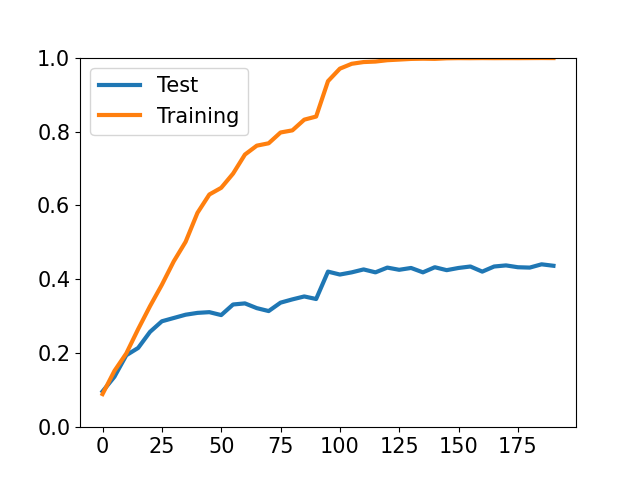
\includegraphics[width = 0.5\textwidth]{figures/wrn_clean_rare_cifar100.png}%
\hfill
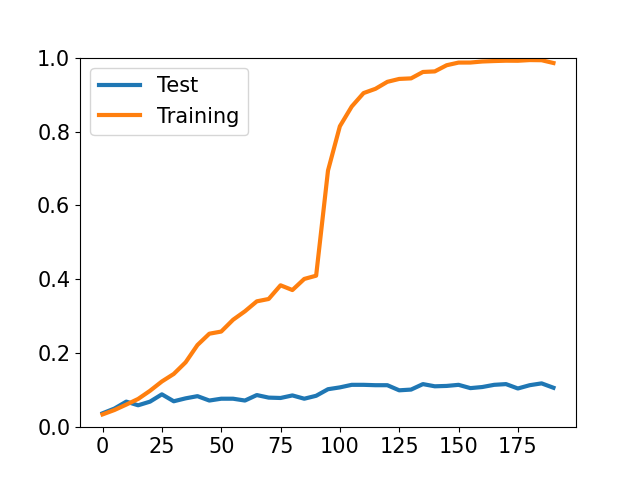
\includegraphics[width = 0.5\textwidth]{figures/wrn_adv_rare_cifar100.png}
\end{minipage}
}
\caption{Clean Accuracy and Adversarial Accuracy on \textbf{Atypical} Set of CIFAR100}
\label{fig:app_1_21}
\vspace{-0.5cm}
\end{figure}

\begin{figure}[h]
\centering
\hspace*{-1cm}
\subfloat[Clean (left) \& Adv Acc. (right) under ResNet18.]{
\begin{minipage}[h]{0.55\textwidth}
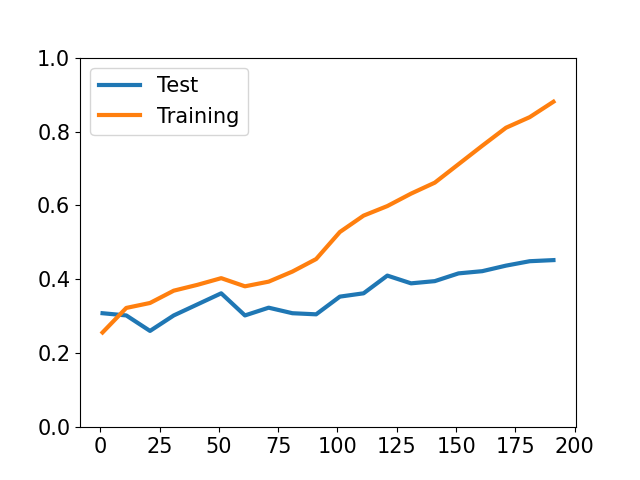
\includegraphics[width = 0.5\textwidth]{figures/pre1_cifar10_adv1_resnet18.png}%
\hfill
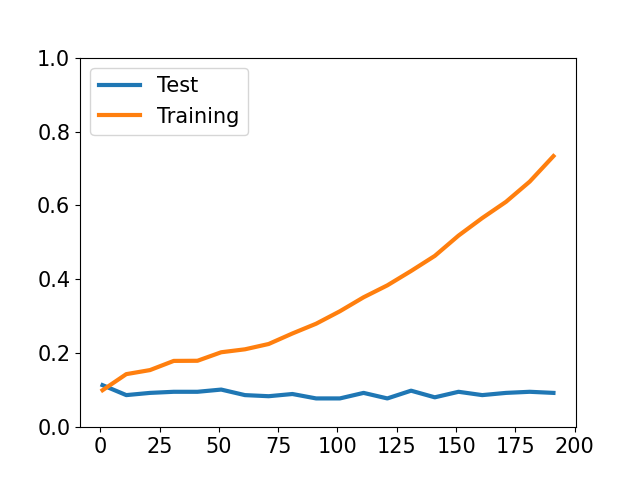
\includegraphics[width = 0.5\textwidth]{figures/pre1_cifar10_adv2_resnet18.png}
\end{minipage}
}
\hspace*{-0.4cm}
\subfloat[Clean (left) \& Adv Acc. (right) under WRN28.]{
\begin{minipage}[c]{0.55\textwidth}
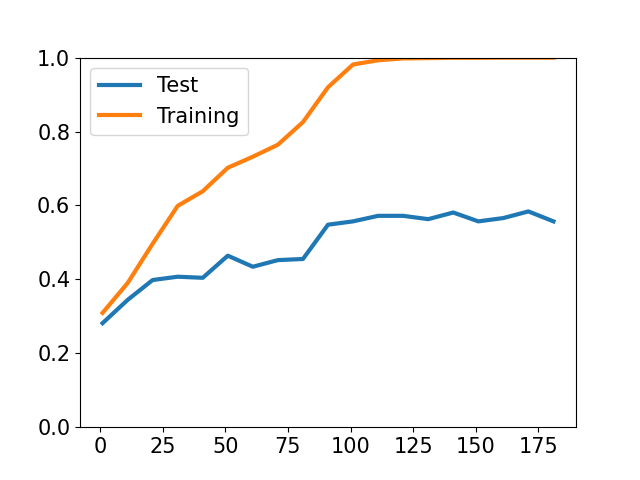
\includegraphics[width = 0.5\textwidth]{figures/pre1_cifar10_adv1_wrn28.png}%
\hfill
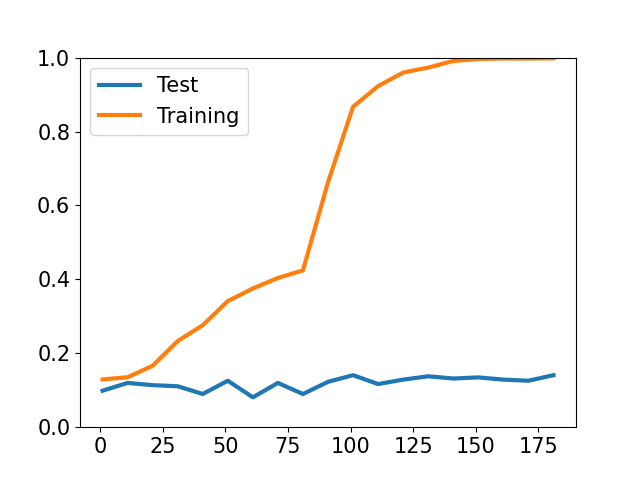
\includegraphics[width = 0.5\textwidth]{figures/pre1_cifar10_adv2_wrn28.png}
\end{minipage}
}
\caption{Clean Accuracy and Adversarial Accuracy on \textbf{Atypical} Set of CIFAR10}
\label{fig:app_1_22}
\vspace{-0.5cm}
\end{figure}

\begin{figure}[h!]
\centering
\hspace*{-1cm}
\subfloat[Clean (left) \& Adv Acc. (right) under ResNet32.]{
\begin{minipage}[h]{0.55\textwidth}
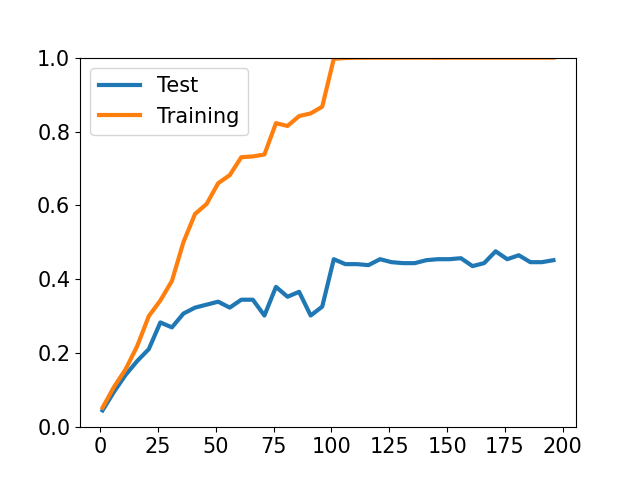
\includegraphics[width = 0.5\textwidth]{figures/pre1_imagenet_adv1_resnet18.png}%
\hfill
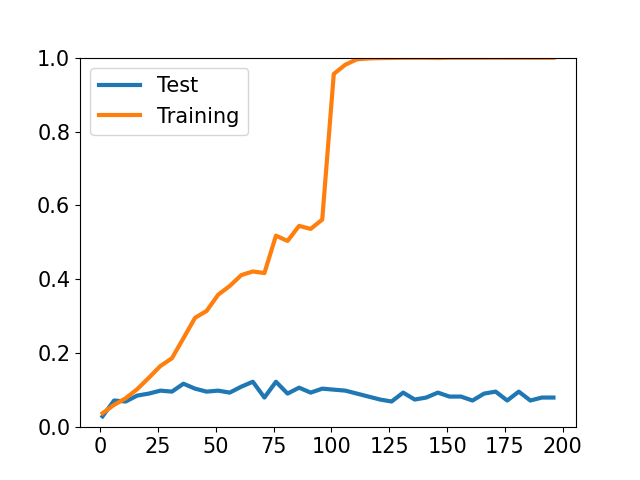
\includegraphics[width = 0.5\textwidth]{figures/pre1_imagenet_adv2_resnet18.png}
\end{minipage}
}
\hspace*{-0.4cm}
\subfloat[Clean (left) \& Adv Acc. (right) under WRN28.]{
\begin{minipage}[c]{0.55\textwidth}
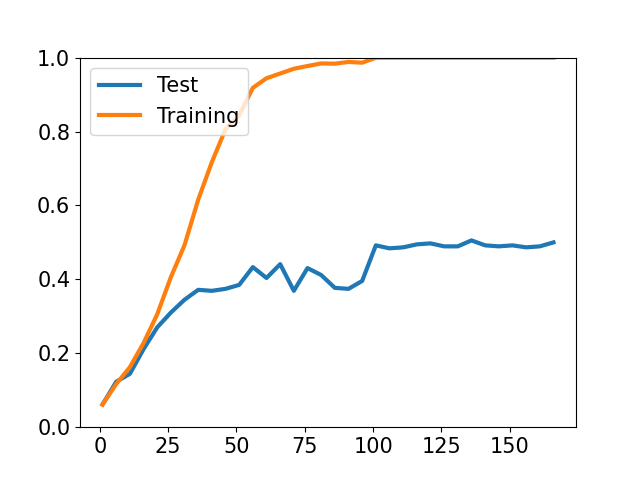
\includegraphics[width = 0.5\textwidth]{figures/pre1_imagenet_adv1_wrn28.png}%
\hfill
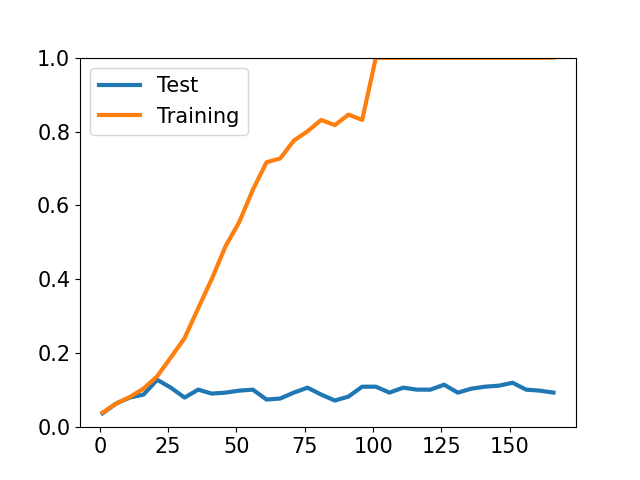
\includegraphics[width = 0.5\textwidth]{figures/pre1_imagenet_adv2_wrn28.png}
\end{minipage}
}
\caption{Clean Accuracy and Adversarial Accuracy on \textbf{Atypical} Set of Tiny~ImageNet}
\label{fig:app_1_23}
\end{figure}



%%%%%%%%%%%%%%%%%%%%%%%%%%%%%%%%%%%%%%%%%%%%%%%%%%%%%%%%%%%%%%%%%%%%%%%%%%%%%%%%%%%%%%%%%%%%%%%%%%%%%%%%%%%%%
\subsection{Additional Results for Preliminary Study - Section~\ref{sec:pre2}}\label{app:pre2}

In this subsection, we provide more experimental results to validate the statement 
in Section~\ref{sec:pre2}, where we state that fitting atypical samples in adversarial training can hurt the performance (clean \& adversarial accuracy) of typical samples.
We provide full empirical results to show that: \textbf{(i)} In traditional ERM, fitting atypical samples will not hurt the models' performance (clean accuracy) of typical samples. \textbf{(ii)} In adversarial training, fitting atypical samples can degrade the clean \& adversarial accuracy of typical samples. \textbf{(iii)} In adversarial training, fitting atypical samples can degrade the quality of learned representations, especially the models' discrimination between classes.
The experimental setting follows Section~\ref{sec:pre2}, where we train the models for several trails on resampled (CIFAR100, CIFAR10, Tiny~ImageNet) datasets: each dataset is constructed with the whole training typical set $\mathcal{D}_\text{typ}$, and a part of the training atypical set $\mathcal{D}_\text{atyp}$ (randomly sample 0\%, 20\% and 100\% in $\mathcal{D}_\text{atyp}$). We evaluate the models' performance on test ``typical'' set $\mathcal{D}'_\text{typ}$ which is defined in Section~\ref{sec:pre2}.

\newpage
\textbf{(i) Additional Results for Preliminary Study - Section~\ref{sec:pre2} In Traditional ERM}

Fig.~\ref{fig:app2_11}, Fig.~\ref{fig:app2_12} and Fig.~\ref{fig:app2_13} report the performance of traditional ERM, trained on different resampled datasets with different amount of atypical samples existed. The figures report the clean accuracy on test typical set of CIFAR100, CIFAR10 and Tiny~ImageNet. We also leave the robustness performance out here as the models are not robust to adversarial attacks. From the results, we can conclude that in traditional ERM, fitting atypical samples will not degrade the models' performance on typical samples. For example, in CIFAR100 dataset, with 100\% atypical samples included (Atypical-100\%)., the accuracy on the test typical set is even slightly higher than the model trained without atypical samples (Atypical-0\%). This conclusion is consistent for all three datasets and model architectures.


\begin{figure}[h]
\centering
\hspace*{-1cm}
\subfloat[ResNet18.]{
\begin{minipage}[c]{0.3\textwidth}
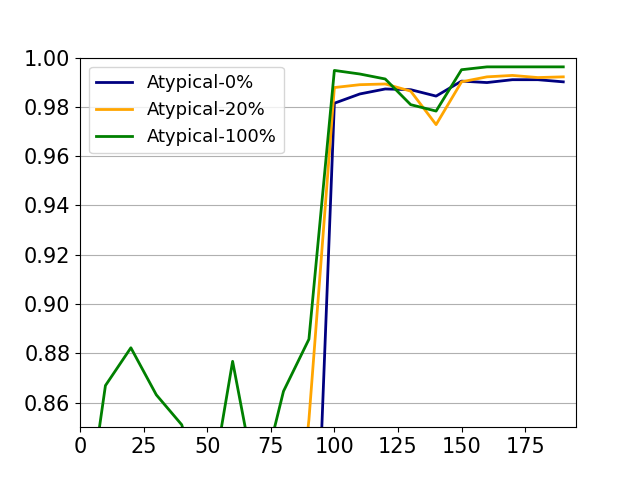
\includegraphics[width = 1.0\textwidth]{figures/pre2_clean_cifar100_ResNet18.png}
\end{minipage}
}
\hspace*{0.4cm}
\subfloat[WRN28.]{
\begin{minipage}[c]{0.3\textwidth}
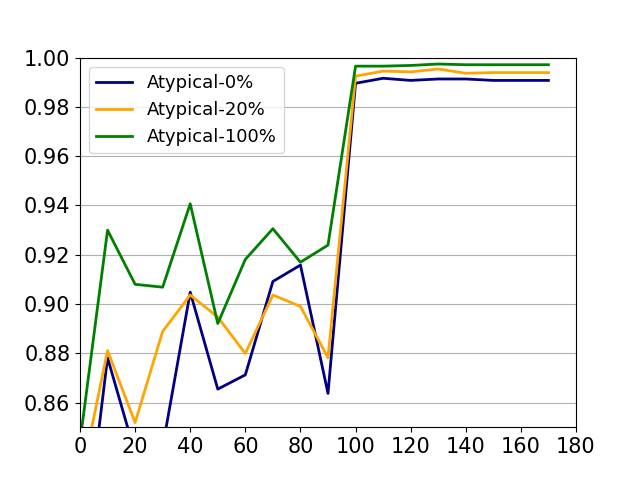
\includegraphics[width = 1.0\textwidth]{figures/pre2_clean_cifar100_WRN28.png}%
\end{minipage}
}
\caption{Clean Accuracy on \textbf{Typical} Set of CIFAR100}
\label{fig:app2_11}
\vspace{-0.5cm}
\end{figure}
%%%%%%%%%%%%%%%%%%%%%%%%%%%%%%%%%%%
\begin{figure}[h]
\centering
\hspace*{-1cm}
\subfloat[ResNet18.]{
\begin{minipage}[c]{0.3\textwidth}
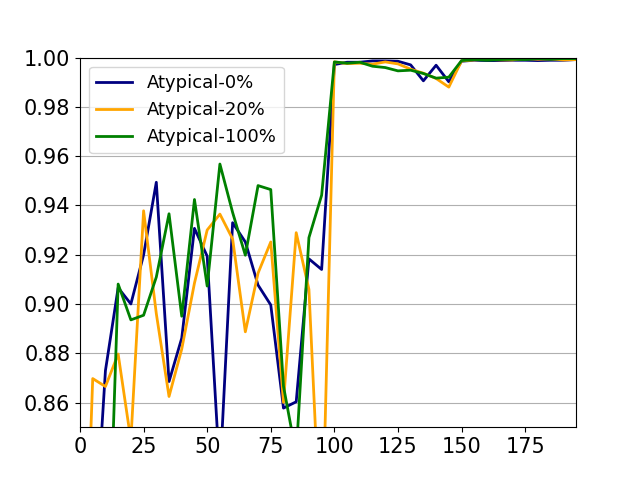
\includegraphics[width = 1.0\textwidth]{figures/pre2_clean_cifar10_ResNet18.png}
\end{minipage}
}
\hspace*{0.4cm}
\subfloat[WRN28.]{
\begin{minipage}[c]{0.3\textwidth}
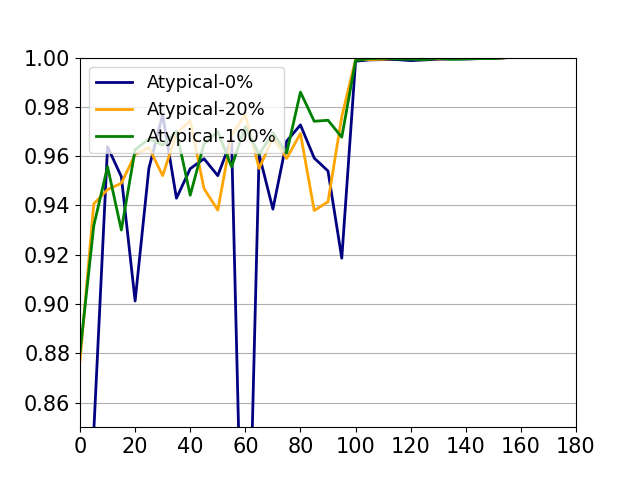
\includegraphics[width = 1.0\textwidth]{figures/pre2_clean_cifar10_WRN28.png}%
\end{minipage}
}
\caption{Clean Accuracy on \textbf{Typical} Set of CIFAR10}
\label{fig:app2_12}
\vspace{-0.5cm}
\end{figure}
%%%%%%%%%%%%%%%%%%%%%%%%%%%%%%%%%%%
\begin{figure}[h!]
\centering
\hspace*{-1cm}
\subfloat[ResNet32.]{
\begin{minipage}[c]{0.3\textwidth}
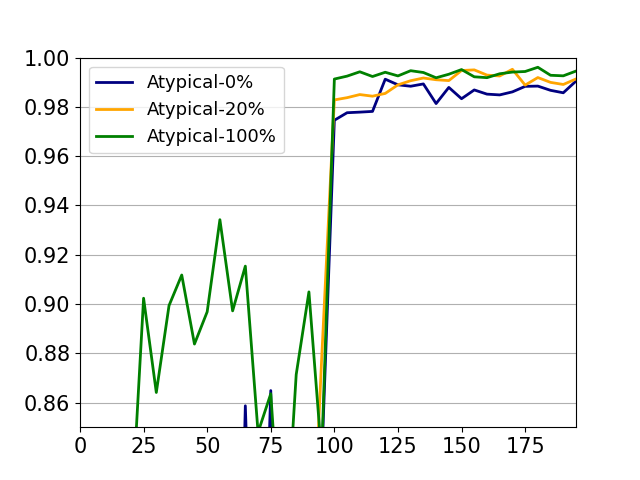
\includegraphics[width = 1.0\textwidth]{figures/pre2_clean_imagenet_ResNet18.png}
\end{minipage}
}
\hspace*{0.4cm}
\subfloat[WRN28.]{
\begin{minipage}[c]{0.3\textwidth}
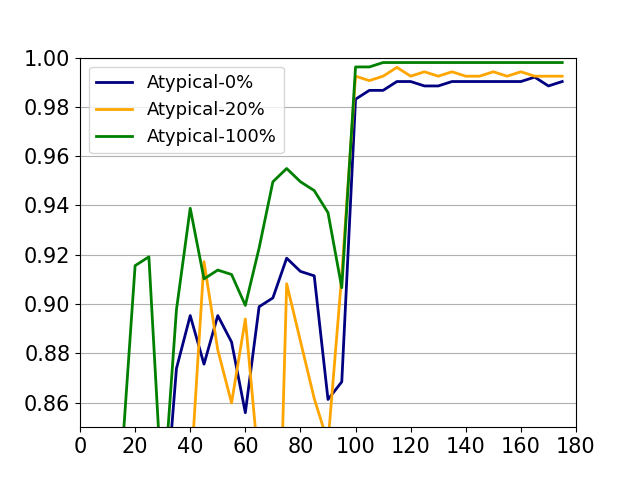
\includegraphics[width = 1.0\textwidth]{figures/pre2_clean_imagenet_WRN28.png}%
\end{minipage}
}
\caption{Clean Accuracy on \textbf{Typical} Set of Tiny~ImageNet}
\label{fig:app2_13}
\end{figure}





%%%%%%%%%%%%%%%%%%%%%%%%%%%%%%%%%%%%%%%%%%%%%%%%%%%%%%%%%%%%%%%%%%%%%%%%%%%%%%%%%%%%%%%%%%%%%%%%%%%%%%%%%%%%%%%%%%%%%%%%%%%%%%%%%%%%%%%%%%%%%%%%%%%%%%%%%%%%%%%%%%%%%%%%%%%%%%%%%%%%%%%%%%
\textbf{(ii) Additional Results for Preliminary Study - Section~\ref{sec:pre2} In Adversarial Training}

Fig.~\ref{fig:pre2_21}, Fig.~\ref{fig:pre2_22} and Fig.~\ref{fig:pre2_23} report the performance of adversarial training, on different resampled datasets with different amount of atypical samples existed. The figures report both clean and adversarial accuracy on test atypical sets of CIFAR100, CIFAR10 and Tiny~ImageNet. Based on the experimental results, we find that including more atypical samples can cause the model have worse performance on typical samples in all three datasets. In datasets with a large portion of atypical samples, such as CIFAR100, the negative effects of atypical samples are more obvious. In CIFAR100, training on datasets with 100\% atypical samples (Atypical 100\%) can cause the clean \& adversarial accuracy drop by $\sim7\%$ and $8\%$, respectively.

\begin{figure}[h]
\centering
\hspace*{-1cm}
\subfloat[Clean (left) \& Adv Acc. (right) under ResNet18.]{
\begin{minipage}[h]{0.55\textwidth}
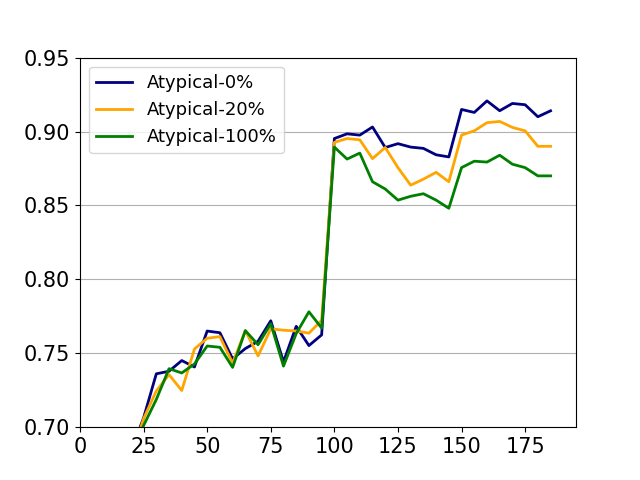
\includegraphics[width = 0.5\textwidth]{figures/poison_clean_ResNet18.png}%
\hfill
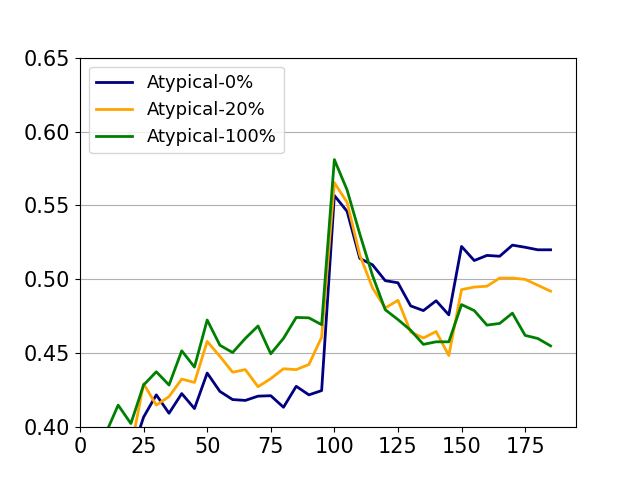
\includegraphics[width = 0.5\textwidth]{figures/poison_adv_ResNet18.png}
\end{minipage}
}
\hspace*{-0.4cm}
\subfloat[Clean (left) \& Adv Acc. (right) under WRN28.]{
\begin{minipage}[c]{0.55\textwidth}
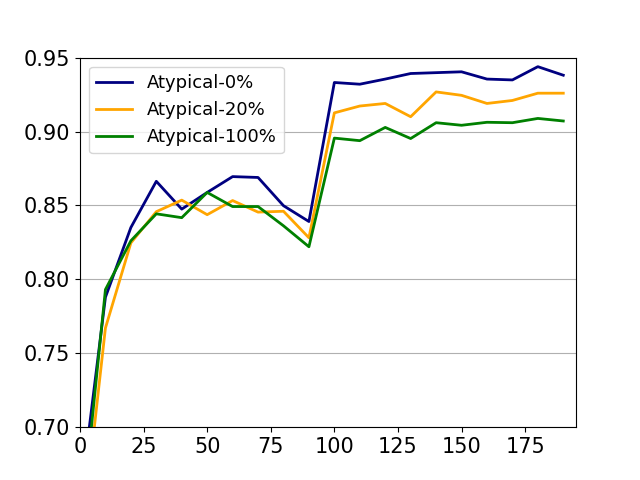
\includegraphics[width = 0.5\textwidth]{figures/poison_clean_WRN.png}%
\hfill
\includegraphics[width = 0.5\textwidth]{figures/poison_adv_WRN.png}
\end{minipage}
}
\caption{Clean Accuracy and Adversarial Accuracy on \textbf{Typical} Set of CIFAR100}
\label{fig:pre2_21}
\vspace{-0.3cm}
\end{figure}
%%%%%%%%%%%%%%%%%%%%%%%%%%%%%%%%%%%%%%%%%%
\begin{figure}[h]
\centering
\hspace*{-1cm}
\subfloat[Clean (left) \& Adv Acc. (right) under ResNet18.]{
\begin{minipage}[h]{0.55\textwidth}
\includegraphics[width = 0.5\textwidth]{figures/pre3_cifar10_adv1_resnet18.png}%
\hfill
\includegraphics[width = 0.5\textwidth]{figures/pre3_cifar10_adv2_resnet18.png}
\end{minipage}
}
\hspace*{-0.4cm}
\subfloat[Clean (left) \& Adv Acc. (right) under WRN28.]{
\begin{minipage}[c]{0.55\textwidth}
\includegraphics[width = 0.5\textwidth]{figures/pre3_cifar10_adv1_wrn28.png}%
\hfill
\includegraphics[width = 0.5\textwidth]{figures/pre3_cifar10_adv2_wrn28.png}
\end{minipage}
}
\caption{Clean Accuracy and Adversarial Accuracy on \textbf{Typical} Set of CIFAR10}
\label{fig:pre2_22}
\vspace{-0.3cm}
\end{figure}
%%%%%%%%%%%%%%%%%%%%%%%%%%%%%%%%%%%%%%%%%%
\begin{figure}[h!]
\centering
\hspace*{-1cm}
\subfloat[Clean (left) \& Adv Acc. (right) under ResNet32.]{
\begin{minipage}[h]{0.55\textwidth}
\includegraphics[width = 0.5\textwidth]{figures/pre3_imagenet_adv1_resnet18.png}%
\hfill
\includegraphics[width = 0.5\textwidth]{figures/pre3_imagenet_adv2_resnet18.png}
\end{minipage}
}
\hspace*{-0.4cm}
\subfloat[Clean (left) \& Adv Acc. (right) under WRN28.]{
\begin{minipage}[c]{0.55\textwidth}
\includegraphics[width = 0.5\textwidth]{figures/pre3_imagenet_adv1_resnet18.png}%
\hfill
\includegraphics[width = 0.5\textwidth]{figures/pre3_imagenet_adv2_wrn28.png}
\end{minipage}
}
\caption{Clean Accuracy and Adversarial Accuracy on \textbf{Typical} Set of CIFAR100}
\label{fig:pre2_23}
\end{figure}


\vspace{2cm}
\textbf{(iii) Additional Results for Preliminary Study - Section~\ref{sec:pre2} Classwise Representation Distance}

Here, we provide additional evidence to show that in adversarial training, fitting atypical samples can degrade the quality of DNN's learned representations (as proposed in Section~\ref{sec:pre2}). In Fig.~\ref{fig:dist1}, Fig.~\ref{fig:dist2} and Fig.~\ref{fig:dist3}, we measure the Cosine Distance (defined in Section~\ref{sec:pre2}) of the representations for (typical) samples from different classes. In these figures, we provide detailed results of both traditional ERM and adversarial training under ResNet18 and WRN28. From the results, we can see that in adversarial training, more atypical samples can cause the smaller classwise Cosine Distance of the models (on their last epochs). Moreover, during the training process of adversarial training, the classwise Cosine Distance first increases and then starts to decrease, especially when there are more atypical samples are fitted. For example, in CIFAR100 under ResNet18, the Cosine Distance starts to decrease at around Epoch 100, which is when many more atypical samples are fitted. These results suggest that, in adversarial training, fitting atypical samples can be an important reason to cause the models to produce poor representations. As a comparison, in Traditional ERM, the classwise Cosine Distance keeps increasing from the first epoch to the last one. Although given the same epoch, the models trained with more atypical samples also have smaller Cosine Distance, they would not harm the model's final performance. It is because the models trained with more atypical samples can also have relatively large classwise Cosine Distance in their last epochs.


%%%%%%%%%%%%%%%%%%%%%%%%%%%%
\begin{figure}[h]
\centering
\hspace*{-1cm}
\subfloat[Traditional ERM under ResNet18 (left), WRN28 (right).]{
\begin{minipage}[h]{0.55\textwidth}
\includegraphics[width = 0.5\textwidth]{figures/dist_cifar100_ResNet18.png}%
\hfill
\includegraphics[width = 0.5\textwidth]{figures/dist_cifar100_wrn28.png}
\end{minipage}
}
\hspace*{-0.4cm}
\subfloat[Adv. Training under ResNet18 (left), WRN28 (right).]{
\begin{minipage}[c]{0.55\textwidth}
\includegraphics[width = 0.5\textwidth]{figures/dist_adv_cifar100_ResNet18.png}%
\hfill
\includegraphics[width = 0.5\textwidth]{figures/dist_adv_cifar100_WRN28.png}
\end{minipage}
}
\caption{Classwise Cosine Distance of Output Representation of \textbf{Typical} Set of CIFAR100}
\label{fig:dist1}
\end{figure}

%%%%%%%%%%%%%%%%%%%%%%%%%%%%
\begin{figure}[h]
\centering
\hspace*{-1cm}
\subfloat[Traditional ERM under ResNet18 (left), WRN28 (right).]{
\begin{minipage}[h]{0.55\textwidth}
\includegraphics[width = 0.5\textwidth]{figures/dist_cifar10_ResNet18.png}%
\hfill
\includegraphics[width = 0.5\textwidth]{figures/dist_cifar10_WRN28.png}
\end{minipage}
}
\hspace*{-0.4cm}
\subfloat[Adv. Training under ResNet18 (left), WRN28 (right).]{
\begin{minipage}[c]{0.55\textwidth}
\includegraphics[width = 0.5\textwidth]{figures/dist_adv_cifar10_ResNet18.png}%
\hfill
\includegraphics[width = 0.5\textwidth]{figures/dist_adv_cifar10_WRN28.png}
\end{minipage}
}
\caption{Classwise Cosine Distance of Output Representation of \textbf{Typical} Set of CIFAR10}
\label{fig:dist2}
\end{figure}


%%%%%%%%%%%%%%%%%%%%%%%%%%%%
\begin{figure}[h!]
\centering
\hspace*{-1cm}
\subfloat[Traditional ERM under ResNet32 (left), WRN28 (right).]{
\begin{minipage}[h]{0.55\textwidth}
\includegraphics[width = 0.5\textwidth]{figures/dist_imagenet_ResNet18.png}%
\hfill
\includegraphics[width = 0.5\textwidth]{figures/dist_imagenet_WRN28.png}
\end{minipage}
}
\hspace*{-0.4cm}
\subfloat[Adv. Training under ResNet32 (left), WRN28 (right).]{
\begin{minipage}[c]{0.55\textwidth}
\includegraphics[width = 0.5\textwidth]{figures/dist_adv_imagenet_ResNet18.png}%
\hfill
\includegraphics[width = 0.5\textwidth]{figures/dist_adv_imagenet_WRN28.png}
\end{minipage}
}
\caption{Classwise Cosine Distance of Output Representation of \textbf{Typical} Set of Tiny~ImageNet}
\label{fig:dist3}
\end{figure}




\section{The Detailed Training Scheme of BAT}\label{app:algorithm}

In this section, we provide the detailed training scheme of BAT in Algorithm~\ref{alg:bat}. In particular, BAT algorithm starts from a randomly initialized neural network. On each mini-batch, it applies PGD attack to generate (training) adversarial examples (Step 5). Following the Eq~\ref{eq:poisoning_score} and Eq~\ref{eq:reweight}, BAT calculates which samples are likely to be \textit{Poisoning Atypical Samples} and their corresponding weight values (Step 6). Under the current mini-batch, next, BAT calculates the \textit{Discrimination Loss} of the typical samples $\mathcal{D}_\text{typ}$ (Step 8). Finally, BAT uses SGD to update the model parameter to minimize the reweighted adversarial loss regularized by $\beta$ times discrimination loss (Step 8).

\begin{algorithm}[h!]
\begin{algorithmic}[1]
\setstretch{1}
\STATE \textbf{Input:} Training dataset $\mathcal{D}$, with typical set $\mathcal{D}_\text{typ} = \{x \in\mathcal{D}; \text{mem}(x) \leq \sigma\}$, atypical set $\mathcal{D}_\text{atyp} = \{x \in\mathcal{D}; \text{mem}(x) > \sigma\}$. Targeted type of adversarial attack: $l_\infty$-$\epsilon$ attack.
Hyperparameters $\alpha, \beta \in \R^+$. \\
\STATE Randomly initialize the network $F$ \\
\REPEAT
\STATE Fetch mini-batch data $\{(x_i,y_i)\}$ at current epoch\\
\STATE Using PGD to generate adversarial training sample  $\{(x_i^\text{adv},y_i)\}$\\
\STATE Calculate Poisoning Score $\textbf{q}(x^\text{adv}_i)$ and weight $w_i$ as in Equation~\ref{eq:poisoning_score} and Equation~\ref{eq:reweight}.
\STATE Calculate Discrimination Loss $\mathcal{L}_{DL}(F)$ within the current mini-batch, as in Equation~\ref{eq:dl}.
\STATE Update $F$ by SGD on the objective: $\mathcal{L}_\text{BAT} = \frac{1}{\sum_i w_i }\sum_i \left[w_i \cdot \mathcal{L}(F(x_i^\text{adv}), y_i)\right] + \beta\cdot\mathcal{L}_{DL}(F)$.
\UNTIL{End of Training}
\caption{The Benign Adversarial Training (BAT) Algorithm}
\label{alg:bat}
\end{algorithmic}
\end{algorithm}



\section{Additional Results for Experiment}\label{app:exp}

In this section, we provide additional experimental results to validate the effectiveness of BAT method. In Table~\ref{tab:resnet18_cifar100} and Table~\ref{tab:wrn28_cifar100}, we provide the results of BAT and baseline models on CIFAR100 dataset under ResNet18 and WRN28 architectures. In Table~\ref{tab:resnet18_imagenet} and Table~\ref{tab:wrn28_imagenet}, we provide the results of BAT and baseline models on Tiny~ImageNet dataset under ResNet32 and WRN28 architectures. In the experiments, we train the models for 160 epochs with learning rate 0.1, momentum 0.9, weight decay 5e-4, and decay the learning rate by 0.1 at the epoch 80 and 120. To have a more comprehensive and reliable adversarial robustness, in addition to PGD adversarial attack~\cite{madry2017towards}, we also measure the model's adversarial accuracy via other attack algorithms, including FGSM attack~\cite{goodfellow2014explaining}, CW attack~\cite{carlini2017towards} and Auto Attack~\cite{croce2020reliable}. The results show that the BAT method can consistently outperform baseline models, as BAT has better clean accuracy vs. adversarial accuracy trade-off. Under ResNet18, the BAT method achieves comparable adversarial accuracy to the best baseline methods, and BATs have the highest clean accuracy. Under WRN28, the BAT method has both higher clean \& adversarial accuracy than the baseline methods.



\begin{table}[h]
\small
\centering
\caption{Performance of BAT vs. Baselines on CIFAR100 Under ResNet18}
\label{tab:resnet18_cifar100}
\begin{tabular}{c|c|ccccc}
\hline
Method & Clean Acc. & FGSM & PGD & CW & AA. \\
\hline
\hline
PGD Train (Best Adv.) & 56.9 & 36.0 & 27.4 & 25.4 & 23.6 \\
PGD Train (Best Clean) & 57.8 & 33.5 & 21.9 & 22.5 & 20.2 \\
TRADES ($1/\lambda = 5$) & 56.6 & 36.5 & 26.9 & 25.3 & 23.9 \\
MART~\cite{wang2019improving} & 51.8 & 36.1 & \textbf{30.4} & 25.8 & \textbf{24.4} \\
GAIRAT~\cite{zhang2020geometry} & 58.2 &36.5 & 27.8 & 25.9 & 23.8\\
\hline
BAT ($\alpha = 1, \beta = 0.2$) & \textbf{59.5} & \textbf{37.3} & 27.3 & \textbf{26.6} & 24.3\\
BAT ($\alpha = 2, \beta = 0.2$) &59.3 & 37.1 & 27.4 & 26.5 & 24.0\\
\hline
\hline
\end{tabular}
\end{table}

\begin{table}[h]
\small
\centering
\caption{Performance of BAT vs. Baselines on CIFAR100 Under WRN28}
\label{tab:wrn28_cifar100}
\begin{tabular}{c|c|ccccc}
\hline
Method & Clean Acc. & FGSM & PGD & CW & AA. \\
\hline
\hline
PGD Train (Best Adv.) & 59.7 & 34.9 & 24.7 & 24.2 & 22.5 \\
PGD Train (Best Clean.) & 59.7 & 34.9 & 24.7 & 24.2 & 22.5 \\
%TRADES ($1/\lambda = 1$) & \textbf{61.3} & 21.9 & \textbf{93.0} & 50.0 & 44.7 & 7.9\\
TRADES ($1/\lambda = 5$) & 57.3 & 34.5 & 24.9 & 24.6 & 22.9 \\
MART~\cite{wang2019improving} & 56.5 & 36.1 & 26.8 & 25.3 & 23.8 \\
GAIRAT~\cite{zhang2020geometry} & 60.2 & 34.8 & 24.4 & 24.8 & 22.9 \\
\hline
BAT ($\alpha = 1, \beta = 0.2$) & \textbf{62.0} & 38.6 & \textbf{28.5} & \textbf{26.5} & \textbf{24.8} \\
BAT ($\alpha = 2, \beta = 0.2$) & 61.4 & \textbf{38.9} & 28.2 & 26.3 & \textbf{24.8} \\
\hline
\hline
\end{tabular}
\end{table}

\begin{table}[h]
\small
\centering
\caption{Performance of BAT vs. Baselines on Tiny~ImageNet Under ResNet32}
\label{tab:resnet18_imagenet}
\begin{tabular}{c|c|ccccc}
\hline
Method & Clean Acc. & FGSM & PGD & CW & AA. \\
\hline
\hline
Adv. Train (Best Adv.) & 56.3 & 37.5 & 32.3 & 29.8 & 29.8\\
Adv. Train (Best Clean) & 58.2 & 36.8 & 30.5 & 28.8 & 28.4\\
TRADES ($1/\lambda = 5$) & 55.4 & 35.2 & 28.8 & 27.0 & 27.0\\
MART~\cite{wang2019improving} & 56.2 & 38.1& \textbf{34.5} & \textbf{31.8} & 32.0\\
GAIRAT~\cite{zhang2020geometry} & 58.4 & 37.3& 30.4 & 28.9 & 29.0\\
\hline
BAT ($\alpha = 1, \beta = 0.2$) & \textbf{59.4} &40.4 &32.0 & 31.5 & 32.0\\
BAT ($\alpha = 2, \beta = 0.2$) & \textbf{59.4} & \textbf{41.3}  &32.9 & \textbf{31.8} & \textbf{32.4}\\
\hline
\hline
\end{tabular}
\end{table}
\begin{table}[h!]
\small
\centering
\caption{Performance of BAT vs. Baselines on Tiny~ImageNet Under WRN28}
\label{tab:wrn28_imagenet}
\begin{tabular}{c|c|ccccc}
\hline
Method & Clean Acc. & FGSM & PGD & CW & AA. \\
\hline
\hline
Adv. Train (Best Adv.) & 58.9 & 35.7 & 31.7 & 30.0 & 30.0  \\
Adv. Train (Best Clean) & 60.0 & 35.1 & 30.1 & 28.8 & 28.5\\
TRADES ($1/\lambda = 5$) & 59.7 & 37.4 & 32.0 & 31.8 & 32.0\\
MART~\cite{wang2019improving} & 58.2 & 41.0 & 35.6 & 33.9 & 34.1 \\
GAIRAT~\cite{zhang2020geometry} & 59.9 & 38.3 & 32.4 & 31.0 & 31.1\\
\hline
BAT ($\alpha = 1, \beta = 0.2$) & 62.3 & 41.6 & 35.8 & 33.7 & 34.3 \\
BAT ($\alpha = 2, \beta = 0.2$) & \textbf{62.4} & \textbf{43.1} &\textbf{37.4} & \textbf{35.3} & \textbf{35.6}\\
\hline
\hline
\end{tabular}
\end{table}



\section{Boarder Impact}\label{app:board}

Nowadays, deep neural networks (DNNs) have been widely applied to solve various machine learning tasks, especially on many safety-critical tasks such as autonomous vehicle~\cite{fagnant2015preparing}, AI healthcare~\cite{jiang2017artificial} and ID authentication~\cite{mohammed2011human}, etc. However, the existence of adversarial attacks~\cite{xu2019adversarial} brings huge threats to the safety of these DNNs' applications. As one of the most successful approaches to defend DNNs against adversarial attacks, adversarial training methods~\cite{madry2017towards, zhang2016understanding} still suffer from several disadvantages. For example, for a DNN model to achieve good adversarial robustness, it usually sacrifices its clean accuracy. Adversarially trained DNNs also present strong overfitting effects. In our study, we draw important findings to explain these drawbacks of adversarial training from the data perspective and empirically validate these issues' relation to atypical samples in the data distribution. Moreover, the currently existed adversarially trained models can only achieve satisfactory performance on simple datasets such as MNIST and CIFAR10. Motivated from our findings, we propose a new method to improve the performance of adversarial training, especially on more complex datasets. We anticipate that our findings and method are helpful for further studies to improve the effectiveness and feasibility of adversarial training and eventually build safer DNNs.


\end{document}
